\documentclass[12pt,a4paper]{article}
\usepackage{amsmath,bm} %mathematische Normen
\numberwithin{equation}{section}
\numberwithin{figure}{section}
\numberwithin{table}{section}
\usepackage[english]{babel} %neue deutsche Rechtschreibung und Formelsatz
\usepackage{amsfonts} %Zus�tzliche Formeln/Symbole/Sonderzeichen...
\usepackage{amssymb} %Formelsatz
\usepackage{graphicx} %Einbinden von Graphiken
\usepackage{wrapfig}
\usepackage{float} %Flussumgebungen
\usepackage[authoryear]{natbib}
%\setcitestyle{authoryear}
\usepackage[font=footnotesize]{caption}
\usepackage{enumerate}
\usepackage[labelfont=bf]{caption}
%\usepackage[utf8]{inputenc} %linux
\usepackage[ansinew]{inputenc} %windows
\usepackage[left=3.0cm,right=2.9cm,top=2.4cm,bottom=2.6cm,includeheadfoot]{geometry}
\usepackage{subcaption}
\begin{document}

\begin{figure}[t]
 \begin{minipage}{0.5\textwidth}
  
\includegraphics[width=\textwidth]{sketches/wwulogo.jpg}
 \end{minipage}
 \hfill
 \begin{minipage}{0.35\textwidth}
  
\includegraphics[width=\textwidth]{sketches/logogeophysik.jpg}
 \end{minipage}
\end{figure}


\author{Veit Magnus L�schow}
\title{Heterogeneous core-mantle boundary heat flux in thermo-chemical core convection}
\date {\today}

\maketitle
\thispagestyle{empty}

\begin{figure}[b!]
 \centering
 \textbf{Masterarbeit im Fach Geophysik}\\
 \vspace{7mm}
 an der \\
 \vspace{7mm}
 \textbf{Wesf�lischen Wilhelms-Universit�t M�nster}
\end{figure}


\newpage
\section*{}
\section*{}
\section*{}
\begin{table*}[b!]
 \begin{tabular}{l l}
  Autor:&Veit Magnus L�schow\\
Matrikelnummer:&370652\\
1. Gutachter: &Prof. Dr. Ulrich Hansen\\
2. Gutachter: &Dr. Stephan Stellmach\\
 \end{tabular}
\end{table*}
\thispagestyle{empty}
\newpage
\tableofcontents
\newpage
 

\section*{Abstract}

Thermal coupling between convection in Earth's mantle and core was proposed to explain asymmetric features of the geomagnetic field during the history of the Earth. The coupling is caused by laterally varying heat flux from the core to the mantle, induced by lateral temperature gradients and compositional heterogeneities in the lower-most mantle. Hints for the laterally varying heat flux were found by seismic tomography as well as by geodynamic models of the mantle.\\
This numerical study aims to explore the influence of these non-uniform boundary conditions, as compared to uniform heat flux boundary conditions on thermo-chemical core convection and some distinct dynamo properties. \\ 
In the model at hand, the heat flux pattern is modeled by a single spherical harmonic of degree and order 2. This setting conserves equatorial symmetry, but imposes azimuthal and polar heat flux gradients. \\
Today, convection in the Earth's core is assumed to be driven predominantly by a combination of thermal and compositional buoyancy sources located at the inner-core boundary. Thermal and compositional diffusivities differ by several orders of magnitude. The resulting differences in the dynamical behavior of the two components demand an approach with distinct transport equations and boundary conditions for temperature and chemical concentration. While fixed flux conditions are applied at the inner and outer thermal boundary, isochemical conditions are used for the compositional field. Simulations for different ratios of thermal and compositional forcing are conducted in order to explore the dependence of the system response on the choice of the forcing scenario. \\
The imposed flux pattern locks the outer core flow to the mantle and therefore breaks its azimuthal symmetry, even for relatively low thermal forcing ratios of 12 \%. As a consequence of the locking, stationary patches of intense radial magnetic field form adjacent to the longitudes of maximum heat flux. Furthermore, the chemical component partly adopts to the geometry of the heat flux pattern and patches of compositionally enriched material form. Despite of the symmetry breaking, stable and dipolar dynamos can be maintained. The magnetic dipole strength is larger and hence rather Earth-like for the cases which are predominantly compositionally driven.
\newpage
\section{Introduction and motivation}
Throughout history, the Earth and its inhabitants have immensely benefited from the existence of a magnetic field in many different ways. The evolution of the Earth's biosphere was made possible by a magnetic shield deflecting harmful solar radiation and since about thousand years, people make use of compasses in the seafaring. Today, the geomagnetic field is of great scientific value since it is one phenomenon out of few that originate in the Earth's outer core while being easily measurable at its surface. A given model of the outer core can be considered realistic only if it is capable of producing a magnetic field that shares common characteristics with the Earth's field. \\
The idea that the geomagnetic field is generated in the electrically conducting liquid outer core (LOC) was first proposed by \citet{larmor1919could} and is known as \textit{geodynamo hypothesis} today. Since then, the geodynamo has been subject to extensive research by means of laboratory and numerical experiments as well as theoretical considerations. That magnetic field can be created by fluid motion in the core, which consists mainly of iron, was promptly accepted while the question how a dynamo process of that extent can be powered, is debated until today. Besides the commonly regarded thermal and compositional convection, tidal and precessional forcing come into account as energy sources \citep{malkus1994energy, tilgner2007kinematic}. The first findings of self-sustaining convection driven numerical dynamo action by \citet{glatzmaier1995three} and \citet{kuang1997earth} can be considered as final validation of the geodynamo hypothesis and hence were a great success. Key features of the geomagnetic field (e.g. a dominant axial dipole, field reversals and the westward drift of the field) could be reproduced in their models. Nevertheless, many questions concerning the dynamo problem remain unanswered. \\
This study concentrates on two of them: (a) How does the mantle as a \textit{heat extracting engine} affect the dynamics? (b) What is the role of a \textit{dual-forcing mechanism} in this context? These questions will be further explained in the subsequent sections and a brief review of the research done in these fields so far will be given.\\ \par \noindent
\subsection*{(a) Core-mantle coupling}
The persistence of patches of intense radial magnetic field at high latitudes (see figure \ref{fig:pomm}) on time scales longer than the typical time scale of the LOC has led to the hypothesis that the mantle (including significantly larger time scales) induces these long-lasting features in the geomagnetic field \citep{bloxham1987thermal, sarson1997influence}. This process is referred to as \textit{core-mantle coupling} and is based on the fact that the amount of heat extracted from the core is controlled by the lower-most region of the overlying mantle. As this region is supposed to be among the most heterogeneous in the Earth \citep{young1987core}, the cooling effect of the mantle on the core can be expected to be non-uniform. \\
\begin{figure}[t]
 \centering
 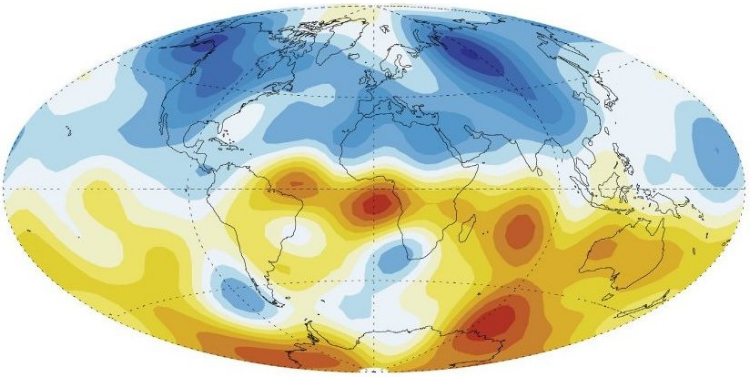
\includegraphics[width=0.8\textwidth]{graphs/pics/pomm_2009.png}
 \caption{Present-day radial geomagnetic field intensity at the CMB, where red represents positive (outward directed) and blue negative (inward directed) values (http://geomag.org/index.html). The two dark blue (dark orange) patches of high intensity field at high latitudes in the northern (southern) hemisphere are of special interest for the present study.}
 \label{fig:pomm}
\end{figure}\noindent
The general idea is that a laterally heterogeneous, hence non-axisymmetric, heat flux from the core to the mantle results in a non-axisymmetric magnetic field geometry, including magnetic flux patches, for example. Evidence for such a non uniform heat flux is provided by two kinds of observations: Lateral gradients in the shear wave velocity close to the core-mantle boundary (CMB), found through seismic tomography, are supposed to result from lateral temperature gradients in that region \citep{su1994degree}. These translate to an increased core-mantle heat flux in relatively cold mantle regions and a decreased heat flux in hot regions. Furthermore, mantle global circulation models (often referred to as mantle GCMs) were recently used to predict the core-mantle heat flux under consideration of many different aspects such as plate tectonics or the chemical composition of the lower-most mantle. According to these results, compositional heterogeneities have an influence on the core-mantle heat flux that adds to the effect of the temperature anomalies mentioned above. Compositionally rich subducted slabs (that are likewise colder than the surrounding material) are characterized by a higher thermal conductivity and therefore further increase the heat flux in regions where those slabs lie adjacent to the CMB \citep{nakagawa2008lateral, nakagawa2013implications}. \\ \par \noindent
\begin{figure}[t]
 \begin{minipage}{0.45\textwidth}
 \centering
 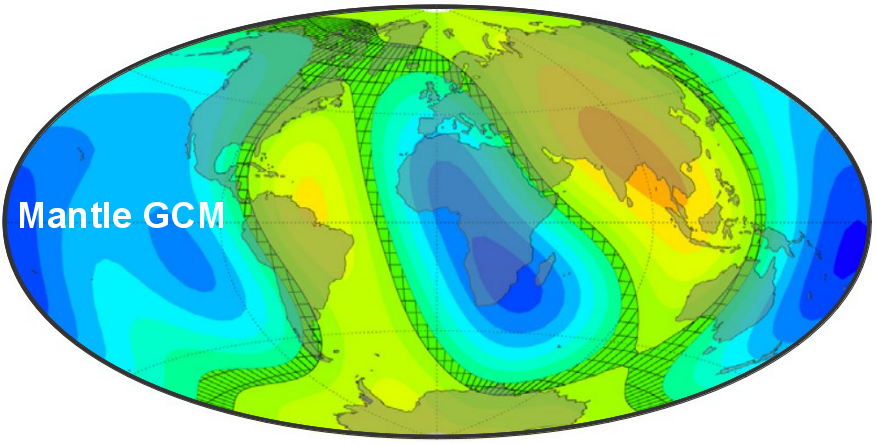
\includegraphics[width=\textwidth]{graphs/olson_pattern.png}
  \end{minipage}
 \begin{minipage}{0.09\textwidth}
\vspace*{\fill}
\centering	
\huge{$\Rightarrow$}
\vspace*{\fill}
  \end{minipage}
   \begin{minipage}{0.45\textwidth}
 \centering
 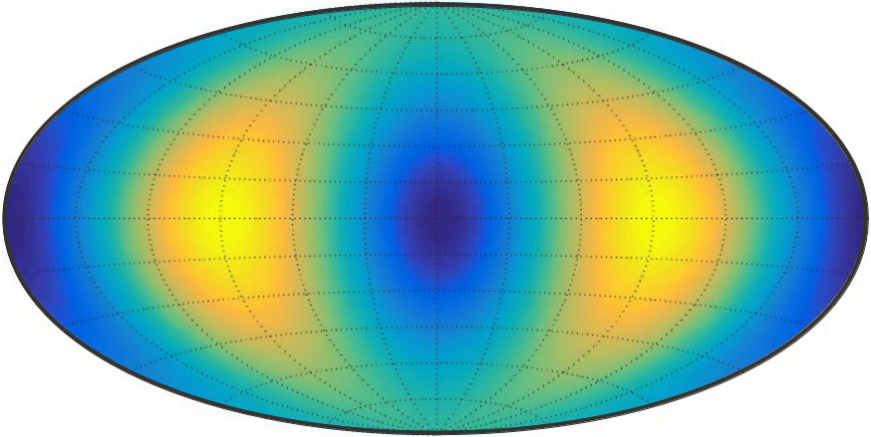
\includegraphics[width=\textwidth]{graphs/Y22_pattern.png}
  \end{minipage}
   \caption{\textbf{Left:} Present-day core-mantle heat flux computed in a mantle GCM (figure changed after \citet{olson2015core}). \textbf{Right:} Heat flux pattern approximation proportional to the spherical harmonic of degree and order 2. This pattern is used in the course of this study as an outer thermal BC. }
\label{fig:approx_pattern}
\end{figure}\noindent
The core-mantle coupling process was explored with respect to a wide range of magnetic field properties: A pioneering study by \citet{bloxham1987thermal} concentrates on anomalies in the secular variation of the geomagnetic field for which a heterogeneous core-mantle heat flux provides a good explanation. The uneven temporal distribution of magnetic field reversals throughout Earth's history is subject to the study of \citet{glatzmaier1999role} and \citet{olson2010geodynamo}. A connection between preferred reversal paths, that can be inferred from paleomagnetic data, and non-uniform core-mantle heat flux is reported by \citet{kutzner2004simulated}. Mars' magnetic dichotomy is addressed by \citet{dietrich2013hemispherical} who use an equatorially antisymmetric heat flux pattern in order to explain the differences in the magnetic field strength in the northern and the southern hemisphere of Mars. \\
A study by \citet{hori2014ancient} addresses the role of core-mantle coupling throughout the history of core evolution. It comes to the result that the present geodynamo is less affected by a non-uniform core-mantle heat flux than earlier dynamos. A stronger influence is found for cases in which internal heat sources make up a major part of the convective forcing, whereas basally driven dynamos show a weaker response to the heat flux pattern. The internally driven scenario is assumed to be realistic for earlier stages of the core, whereas the present dynamo is expected to be predominantly powered by bottom buoyancy sources.\\ 
\citet{olson2002time} and \citet{aubert2007detecting} recently examined long-term averaged flow and magnetic field properties  since those reveal a stronger signature of the heat flux pattern. Their results suggest that the structure of the flow pattern can be properly explained with a thermal wind balance. A prominent feature of the flow is the existence of stationary, anti-clockwise rotating vortex columns which are made responsible for the formation of stationary magnetic flux patches. The present study aims to give a more detailed analysis of the latter point, likewise regarding long-term averages.  \\ \par \noindent
For today's core, tomography as well as the mantle GCMs roughly agree on the geometry of the core-mantle heat flux heterogeneity that reveals a dominance of the spherical harmonic mode of degree and order 2 \citep{masters2000relative, romanowicz2002superplumes}. The study at hand makes use of this fact and applies a fixed flux boundary condition (BC) at the CMB that is proportional to the spherical harmonic $\mathcal{Y}_2^2$ in order to model the non-uniform core-mantle heat flux. Figure \ref{fig:approx_pattern} (left) shows the present-day heat flux, inferred from a mantle GCM \citep{olson2015core}, and its equivalent in the model used in this study (right). It becomes clear that the $\mathcal{Y}_2^2$ BC is a reasonable first order approximation to the situation at the CMB. \\
However, this approach is not meant to produce magnetic field data that is quantitatively comparable to measurements of the geomagnetic field. The aim is rather to understand the principal way in which the imposed flux pattern constrains the flow and herewith connected properties such as the magnetic field morphology or the distribution of the light element. This issue will be regarded in the context of a dual forcing scenario. 
\subsection*{(b) A thermo-chemical approach to dynamo modeling}
The outer core of the Earth is assumed to be composed of an iron-nickel alloy that contains a portion of light elements. Their exact composition is still unknown but silicon and oxygen seem likely to make up a great part of it \citep{tsuno2013simultaneous}. Originating at the inner-core freezing front where they are released during the crystallization process, their appearance in the outer core is a direct consequence of the inner-core growth. If injected into the core fluid, they decrease its density, so that the light elements are a potential source of buoyancy at the inner-core boundary (ICB). It exists general agreement on the assumption that such compositional buoyancy sources at the bottom of the outer core account for a significant part of the total convective forcing \citep{braginsky1995equations}. The second basal source of buoyancy is latent heat, likewise being released at the inner-core freezing front. The role of internal heat sources is expected to play a minor role for today's core \citep{nimmo2007thermal} and is therefore not regarded in this study.  \\
It is common practice in the dynamo community to combine compositional and thermal buoyancy sources in one variable named \textit{codensity}. An important argument for this approach is based on the presumably turbulent nature of core convection. In order to overcome the herewith connected small-scale structure of the flow, artificially high turbulent diffusivities are introduced \citep{braginsky1995equations}. This leads to the assumption that differences in the diffusivities of composition and temperature average out and therefore the two can be treated jointly. \\
In the Earth's core, the diffusivity of heat is expected to be several orders of magnitude larger than that of the light component, which translates to a difference in their associated Prandtl numbers (the ratio of viscosity to diffusivity) of $\sim\!10^3$ \citep{braginsky1995equations}. Several studies recently addressed the influence of the Prandtl number on certain system properties such as the mean flow scales \citep{cardin1992experimental} or the morphology of the resulting magnetic field \citep{simitev2005prandtl}. A significant dependence on that system parameter was reported by all of them. Following these results, a few authors explored models in which temperature and composition act as two distinct driving agents (in the following referred to as dually forced or thermo-chemical models). \citet{trumper2012numerical} found a drastic change in the mean flow properties when varying the ratio of thermal to compositional driving forces in a non-magnetic convection system. A dually forced dynamo model was subject to the work of \citet{takahashi2014double}, who found a sensible dependence of the strength of the magnetic dipole component on the thermo-chemical forcing ratio. \\
In the scope of this study, the possibility to apply two distinct sets of BCs for the thermal \textit{and} the compositional component, especially at the CMB, is the strongest argument in favor of a thermo-chemical approach. According to the previous discussion, it seems reasonable to assume a laterally heterogeneous core-mantle heat flux. In contrast to that, the situation for the compositional component is less clear. \citet{braginsky1995equations} suppose that the CMB is impermeable for the light element, hence a zero-flux condition the most realistic choice. Likewise, the sedimentation of chemical constituents as well as chemical reactions at the CMB are discussed as sinks for the compositional field \citep{buffett2007core}. This would suggest a non-zero fixed flux condition. However, from the current point of view there is no reason to suppose that the compositional BC is identical to the heterogeneous heat flux condition that is applied to the temperature field. This is an assumption intrinsic to codensity models that address a heterogeneous core-mantle heat flux, since they combine composition and temperature and therefore their respective BCs in one variable.\\ \par \noindent
This study aims to explore a thermo-chemically driven model of the LOC in which an non-uniform fixed flux condition is applied to the outer thermal boundary, while the inner thermal and both compositional BCs remain uniform. The guiding questions are:
\begin{enumerate}[(a)]
 \item How does the flow field change under the influence of the heterogeneous BC? How do changes in the flow field affect related system properties such as the distribution of the light element? 
 \item What is the exact mechanism behind the formation of magnetic flux patches in systems with non-uniform core-mantle heat flux? How does a second, uniformly forcing component affect this mechanism?
 \item What can be expected to be the role of a heat flux pattern in a Earth-like parameter regime?
\end{enumerate} 
\subsection*{}
\textbf{Outline of this thesis} This thesis consists of six sections. Section \ref{sec:modeling} provides a brief introduction into the mathematical model that is used as well as to the applied numerical solution scheme. The non-uniform heat flux pattern is described in greater detail (section \ref{sec:flux_pattern}). Additionally, section \ref{sec:modeling} contains the diagnostic quantities that are used in the subsequent sections. Non-magnetic thermo-chemical convection is studied in section \ref{sec:thermo-chemical}, where special attention is paid to the dynamics of the flow. Section \ref{sec:dynamo} deals with thermo-chemical dynamo action. The generation of magnetic flux patches is regarded in the context of a dual forcing scenario. A summary of the results will be given in section \ref{sec:summary}, section \ref{sec:conclusion} contains the conclusion and an outlook.


\newpage
\section{Modeling core convection and dynamo action}
\label{sec:modeling}
Rotating convection and dynamo action in Earth's core is a topic that has been extensively studied (see \citet{jones2011planetary} for a recent review). There exist various ideas of how to formulate a set of equations that depicts all relevant physical processes and that is still as simple and therefore numerically economical as possible. Computation time is the limiting factor when it comes to the question how realistic models of the outer core can be. The gap between the relevant physical parameters supposed for the Earth (see table \ref{tab:parameter}) and the parameters that are in range of numerical modeling is still big. It cannot be expected that this gap will be closed only with the help of the increasing computational resources that will become available within the next years. Alternatives to waiting for faster computers that allow to explore Earth-like parameters have to be found. Asymptotic models are one possibility already revealing promising results (e.g. \citet{stellmach2014approaching}).\\
An aspect that is closely related to the numerical costs and therefore to the accessible parameter range is the choice of the geometry. Most models are either Cartesian with periodic BC or spherical shell models. The latter are more realistic for the Earth but numerically more costly and therefore even less Earth-like with regard to computational feasible parameters. In this work, a spherical model is used in order to be as Earth-like as possible in a geometrical way. As a trade-off, parameter regimes in which Cartesian models could advance, are unreachable here. Typical values for the relevant control parameters in the LOC and in this study can be found in table \ref{tab:parameter}. \\
The electrically conducting LOC is modeled. It is enclosed by the ICB at the bottom and the CMB at the top. Convection is driven by supercritical thermal and compositional gradients across the sphere. For the compositional component, fixed chemical concentrations at the ICB and the CMB are imposed (Dirichlet BC). The thermal forcing is maintained by introducing a fixed in- and outflux of heat (Neumann BC). The heat flux at the CMB is laterally heterogeneous, i.e., there exist regions of higher and lower heat flux than the lateral average. The inner core and mantle are assumed to be electrically insulating and therefore have no influence on the evolution of magnetic fields. \\ 
In the following, all relevant equations are introduced. There exist numerous detailed derivations so that the description will be held relatively short, here. The according references will be given in each section, a good overview can be found in \citet{braginsky1995equations}. \\
\begin{table}[b!]
 \centering
 \begin{tabular}{l|l|l}
 Control parameter & \textbf{Rayleigh number} & \textbf{Ekman number }\\
 \hline
 Earth's core & $10^4\times\textrm{Ra}_\textrm{crit}$ & $10^{-15}-10^{-14}$ \\
 Present model & $(4-24)\times\textrm{Ra}_\textrm{crit}$ &$10^{-5} - 10^{-4}$\\
 \end{tabular}
 \caption{Typical values of control parameters assumed for the LOC and the values regarded in this study \citep{christensen2011geodynamo}.}
 \label{tab:parameter}
\end{table}

\subsection{Frame of reference}
The LOC is modeled in a spherical shell with an inner radius R$_i$ and an outer radius R$_o$ (see figure \ref{fig:FOC}(a)). It is bounded by the ICB at the bottom and the CMB at the top. The shell thickness is chosen according to what is supposed for today's state of the Earth and is defined over the ratio between R$_i$ and R$_o$: $ a = $ R$_i$ / R$_o$ = 0.35.\\
The system is constantly rotating about the z-axis of a Cartesian system with an angular velocity $\Omega$ that is invariant in time. The effect of rotation on the frame of reference will be discussed later in the context of the equation of motion in section \ref{sec:momentum}. In the course of this study, spherical coordinates are used (see figure \ref{fig:FOC}(b) for the definition of the unit vectors).  \\
\begin{figure}[H]
 \begin{minipage}{0.42\textwidth}
  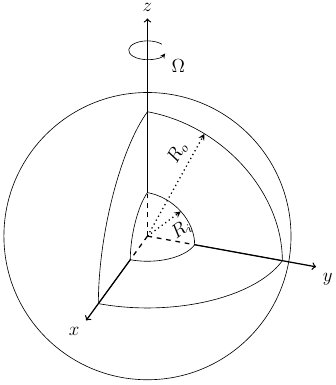
\includegraphics[width=\textwidth]{sketches/spherical_coord.jpg} 
  \caption*{(a)}
 \end{minipage}
 \hfill
\begin{minipage}{0.47\textwidth}
  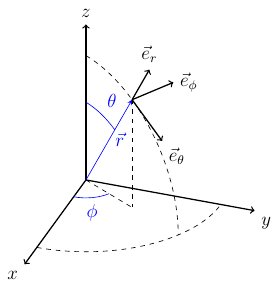
\includegraphics[width=\textwidth]{sketches/spherical_coord2.jpg} 
  \caption*{(b)}
  \end{minipage}
  \caption{(a) Sketch of the LOC. It is bounded by the two spheres of radii R$_i$ and R$_o$. The rotation axis is the cartesian $z$-axis. (b) This work uses spherical coordinates with unit vectors $ \bm{e_r}$, $\bm{e_\Phi}$ and $\bm{e_\vartheta}$ \citep{trumper2014thermo}.}
  \label{fig:FOC}
\end{figure}
\subsection{Equation of continuity}
\label{sec:continuity}
Per definition, the mass $ \mathcal{M} $ of a material volume $ \mathcal{V}(t) $ with a density $\rho$, moving with a velocity $ \bm u(\bm r,t) $ in a fluid, is conserved: 
\begin{equation}
\frac{d \mathcal{M}(\mathcal{V})}{dt} = \frac{d}{dt} \int_{\mathcal{V}(t)} \rho(\bm r,t) d^3r  = 0
\end{equation}
Using Reynold's transport theorem and then applying Gauss's theorem, this yields
\begin{equation}
  \int_{\mathcal{V}(t)} \frac{\partial \rho}{\partial t} d^3r + \oint_{\partial \mathcal{V}(t)} \rho \bm u \cdot \bm {ds} = \int_{\mathcal{V}(t)} \left[ \frac{\partial \rho}{\partial t} + \bm \nabla \cdot (\rho \bm u) \right] d^3r = 0.
\end{equation}
Since this has to hold for all possible material volumes $\mathcal V$, one gets
\begin{equation}
 \frac{\partial \rho}{\partial t} + \bm \nabla \cdot (\rho \bm u) = 0,
\end{equation}
the general form of the equation of continuity. The introduction of the \textit{material derivative} $\frac{D }{Dt} = \frac{\partial }{\partial t} + \bm u \cdot \bm \nabla$ suggests another useful formulation:
\begin{equation}
 \frac{\partial \rho}{\partial t} + \rho \bm \nabla \cdot \bm u + \bm u \cdot \bm \nabla \rho =   \frac{D \rho}{D t} + \rho \bm \nabla \cdot \bm u = 0.
\end{equation}
\subsection{Equation of momentum}
\label{sec:momentum}
In an inertial, non rotating frame of reference, the change of momentum of a material volume $\mathcal{V}$ can be written as 
{\allowdisplaybreaks
\begin{align*}
 \frac{d}{dt} \int_{\mathcal{V}(t)} (\rho u_j) d^3r &= \int_{\mathcal{V}(t)} \left[ \frac{\partial (\rho u_j)}{\partial t} + \frac{\partial}{\partial x_i} (\rho u_j)u_i \right]d^3r \\
    &=   \int_{\mathcal{V}(t)} \left[ \rho \frac{\partial u_j}{\partial t} + u_j \frac{\partial \rho}{\partial t}  +\rho u_j \frac{\partial u_i}{\partial x_i} + u_i \rho \frac{\partial u_j}{\partial x_i} + u_i u_j \frac{\partial \rho}{\partial x_i} \right] d^3r\\
    &= \int_{\mathcal{V}(t)} \left[ u_j\left( \frac{\partial \rho}{\partial t} + \rho \bm \nabla \cdot \bm u + \bm u \cdot \bm \nabla \rho \right) + \rho \left( \frac{\partial u_j}{\partial t} + \bm u \cdot \nabla u_j \right) \right]d^3r \\
    &= \int_{\mathcal{V}(t)}  \rho \frac{D u_j}{D t} d^3r.
\end{align*}}
Such a change can be induced by either \textit{volume forces} $\bm f$ or \textit{surface forces} $\bm t$:
\begin{equation}
 \int_{\mathcal{V}} \rho \frac{D \bm u}{D t} d^3r = \int_{\mathcal{V}} \bm f d^3r + \oint_{\partial \mathcal{V}} \bm t ds
 \label{eq:force_balance1}
\end{equation}
If a frame of reference is rotating - as in this case - it is no longer an inertial system and therefore pseudo forces have to be expected. Under the assumption of a constant rotation with the angular velocity $\Omega$ and a fixed rotation axis parallel to the Cartesian z-axis, the change of a quantity $\bm P$ in the rotating frame of reference and its change in the non rotating inertial frame relate as
\begin{equation}
\left(\frac{d \bm P}{dt}\right)_F = \left(\frac{d \bm P}{dt}\right)_R + \bm \Omega \times \bm P,
\label{eq:frame_of_reference_rule}
\end{equation}
where the subscripts $F$ and $R$ denote the \textit{fixed} and the \textit{rotating} frame. Applying rule \eqref{eq:frame_of_reference_rule} twice to a position vector $\bm r$ yields 
\begin{equation}
 \bm a_F = \bm a_R + 2\bm \Omega \times \bm u_R + \bm \Omega \times (\bm \Omega \times \bm r)
 \label{eq:frame_of_reference_accelerations}
\end{equation}
for an acceleration $\bm a$. $2\bm \Omega \times \bm u_R$ is the Coriolis force and $\bm \Omega \times (\bm \Omega \times \bm r)$ the centripetal force. \\
With equation \eqref{eq:frame_of_reference_accelerations}, $\frac{D \bm u}{D t}$ can be transferred from the inertial frame to the frame of reference:
\begin{equation}
 \frac{D \bm u_F}{D t} = \frac{D \bm u_R}{D t} + 2\bm \Omega \times \bm u_R + \bm \Omega \times (\bm \Omega \times \bm r)
 \label{eq:frame_of_reference_material}
\end{equation}
From now on, the subscripts $F$ and $R$ will be cut and all quantities will be measured in the rotating frame. Using equation \eqref{eq:frame_of_reference_material}, equation \eqref{eq:force_balance1} changes to
\begin{align}
  \int_{\mathcal{V}} \rho \frac{D \bm u}{D t} d^3r = \int_{\mathcal{V}} \bm f d^3r + \oint_{\partial \mathcal{V}} \bm t ds 
  - \int_{\mathcal{V}} \rho \left( 2\bm \Omega \times \bm u + \bm \Omega \times (\bm \Omega \times \bm r) \right) d^3r.
  \label{eq:force_balance2}
\end{align}
Another pseudo force that generally appears in rotating systems is the \textit{Poincar\'{e} force}. In a geophysical context, \textit{precession driven flows} are the most prominent example where it plays a dominant role \citep{Tilgner2007, ernst2013finite}. Its introduction into this model would crucially increase the level of complexity and therefore it is neglected here. \\ \par \noindent
The \textit{Cauchy Theorem} relates the surface forces $\bm t$ to the stress tensor $\underline{\tau}$ linearly via $\bm t = \underline{\tau} \cdot \bm n$, where $\bm n$ is the surface normal vector. The surface term in equation \eqref{eq:force_balance2} can thus be transformed to
\begin{equation}
 \oint_{\partial \mathcal{V}} \bm t ds = \int_{\mathcal{V}} \bm \nabla \cdot \underline{\tau} d^3r,
\end{equation}
where $\bm \nabla \cdot \underline{\tau} = -\bm \nabla p + \mu \bm \nabla^2 \bm u$ will be used as a reasonable simplification in the context of the Boussinesq approximation (see section \ref{sec:boussinesq}). This expression of $\bm \nabla \cdot \underline{\tau}$ is valid for Newtonian fluids and it is based on the assumption of a solenoidal velocity field ($\bm \nabla \cdot \bm u = 0$) and a homogeneous dynamic viscosity $\mu $ throughout the fluid. \\ \par \noindent
The body forces $\bm f$ are the \textit{buoyancy force} $\bm f_g =  \bm g \rho$ and the \textit{Lorentz force} $\bm f_l = \bm j \times \bm B$. The latter will be discussed in section \ref{sec:lorentz}.\\
\par \noindent
In the following, the gravitational field $\bm g$ will be discussed in more detail. As mentioned before, the system underlies an asymmetric heat flux at the CMB. This results in an asymmetric temperature field for which the penetration depth of the temperature perturbation to a spherically symmetric solution depends on the amplitude of the heat flux heterogeneity. Following the linear equation of state from the Boussinesq approximation (see equation \eqref{eq:equation_of_state} in section \ref{sec:boussinesq}), this results in a density variation proportional to the temperature variation: $\delta {\rho} \sim \delta {T}$. Figure \ref{fig:density_var} shows a sketch of the density variation along the equator at the CMB, evoked by the boundary induced lateral temperature variation.
\begin{figure}[H]
 \centering
 \includegraphics[scale = 0.24]{sketches/density_var.pdf} 
 \caption{Sketch of the density along the equator, near the CMB. The deviation (black) from the average density (red) results from the asymmetric heat flux at the CMB which has an asymmetric temperature field as a consequence. }
 \label{fig:density_var}
\end{figure} \noindent
The density field $\rho$ can be split into a spherically symmetric part $\mathring{\rho}(r)$, that only depends on the radial level $r$ and the density variation due to the heat flux pattern $\delta \mathring{\rho}(r,\vartheta,\phi)$:
\begin{equation}
 \label{eq:density_split}
 \rho(r,\vartheta,\phi) = \mathring{\rho}(r) + \delta \mathring{\rho}(r,\vartheta,\phi).
\end{equation}
In case of a heat flux pattern proportional to the spherical harmonic $\mathcal{Y}_2^2$, the dependence of $\delta \mathring{\rho}$ on $\phi$ is $\pi$-periodic (see Figure \ref{fig:density_var}). Thus, it can be expressed by the product $\delta \mathring{\rho}(r,\vartheta,\phi) = \mathcal{C}(r,\vartheta) \cdot cos(2\phi)$, where $\mathcal{C}$ is only a function of $r$ and $\vartheta$. \\ \par \noindent
\textit{Gauss's} gravity law \citep{blakely1996potential} states
\begin{equation}
 \label{eq:gauss}
 \bm \nabla \cdot \bm g = - 4\pi G \rho(r,\vartheta,\phi).
\end{equation}
Integration over a sphere of radius $r$ and application of Gauss's theorem yields
{\allowdisplaybreaks
\begin{align}
% \label{eq:grav_balance}
\nonumber
\int\limits _{\mathcal{V}(r)} \bm \nabla \cdot \bm g dV &= \int\limits_0^\pi \int\limits_0^{2\pi} r^2sin(\vartheta )d\vartheta d\phi \bm g \cdot \bm{e_r}= - 4 \pi G \int\limits_0 ^r \int\limits_0^\pi \int\limits_0^{2\pi} sin(\vartheta) r'^2 \rho(r,\vartheta,\phi) \, dr' d\vartheta d\phi\\
\nonumber
&=- 4 \pi G \int\limits_0 ^r \int\limits_0^\pi \int\limits_0^{2\pi} sin(\vartheta) r'^2 [\mathring{\rho}(r') + \delta \mathring {\rho}(r',\vartheta,\phi)] \, dr' d\vartheta d\phi \\
\nonumber
&=-8\pi^2 G\int\limits_0^r \mathring{\rho}(r') \, dr' -  4 \pi G \int\limits_0 ^r \int\limits_0^\pi sin(\vartheta) r'^2 \mathcal{C}(r',\vartheta) \left( \int\limits_0^{2\pi} cos(2\phi) d\phi \right) \, dr' d\vartheta \\
\nonumber
&= -8\pi^2 G\int\limits_0^r \mathring{\rho}(r') \, dr'
\end{align}}
Because the integration of $\delta \mathring {\rho}(r',\vartheta,\phi)$ over $\phi$ drops out for every value of $r$ and $\vartheta$, $\bm g$ can be expressed by
\begin{equation}
\label{eq:gravity_field}
 g(\bm r) = -\frac{4 \pi G}{r^2}\int_0^r \mathring{\rho}(r')r'^2 \, dr
\end{equation}
and it is worth noticing that $\bm g$ has the same form as in the spherical symmetric case \citep{blakely1996potential}.\\
The buoyancy force term $\bm g \rho$ will be further discussed in section \ref{sec:boussinesq}.

\subsection{Maxwell equations, Lorentz force and induction equation}
\label{sec:lorentz}
The LOC consists of a metallic and therefore conducting fluid. Electric currents may evolve, create magnetic fields and these again may generate currents and affect the flow field. The induction equation is a transport equation for magnetic fields $\bm B$ that are 'hosted' by a fluid moving with a velocity $\bm u$. The Lorentz force characterizes the influence of the magnetic field on the flow field, whereas the Maxwell equations describe how electric and magnetic fields interact through charges and currents. They form a basis for the 'magnetic part' of magnetohydrodynamics.\\
In the scope of core convection, a reduced form of the Maxwell equations (Pre-Maxwell equations) suffices \citep{davidson2001introduction}: 
\begin{subequations} \label{eq:maxwell}
\begin{align}
 \label{eq:ampere}
 \bm \nabla \times \bm B &= \mu_0 \bm j \quad & \text{(Amp\`{e}re's law)} \\
 \label{eq:charge_conservation}
 \bm \nabla \cdot \bm j &= 0 \quad & \text{(Charge conservation)}\\
\label{eq:faraday}
 \bm \nabla \times \bm E &= - \frac{\partial \bm B}{\partial t} \quad & \text{(Faraday's law)}\\
 \label{eq:no_magnetic_monopoles}
 \bm \nabla \cdot \bm B &= 0 \quad & \text{(No magnetic monopoles)} 
\end{align}
\end{subequations}
Additionally, an extended version of \textit{Ohm's law} for moving conductors
\begin{equation}
\label{eq:ohm}
 \bm j = \sigma (\bm E + \bm u  \times \bm B)
\end{equation}
and an expression for the \textit{Lorentz force}
\begin{equation}
\label{eq:lorentz}
 \bm f_l = \bm j \times \bm B = \frac{1}{\mu_0} (\bm \nabla \times \bm B \times \bm B)
\end{equation}
are needed. $\bm E$ describes the electric field, $\bm j$ the current density, $\mu_0$ the vacuum permeability and $\sigma$ the conductivity of the fluid.\\
The \textit{induction equation} can be derived using equations \eqref{eq:faraday}, \eqref{eq:ohm} and the solenoidal character of $\bm B$, \eqref{eq:no_magnetic_monopoles} and $\bm u$:
\begin{equation}
 \label{eq:induction}
 \frac{\partial \bm B}{\partial t} = \bm \nabla (\bm u \times \bm B) + \eta \bm \nabla^2 \bm B,
\end{equation}
where $\eta = \frac{1}{\sigma \mu_0}$ is the magnetic diffusivity.

\subsection{Conservation of energy and the light component}
\label{sec:internal_energy}
The conservation of internal energy in a fluid reads
\begin{equation}
 \label{eq:internal_energy}
 \rho \frac{D e}{D t} =  -\bm \nabla \cdot \bm q_\textrm{\tiny T} - p(\bm \nabla \cdot \bm u) + \Phi,
\end{equation}
where the internal energy per unit mass is described by $e$. It can be changed by either \textit{volume compression} $- p(\bm \nabla \cdot \bm u)$, \textit{viscous dissipation} $\Phi$ or a \textit{heat flux} $\bm q_\textrm{\tiny T}$ through the fluid surface. In the context of the Boussinesq approximation (section \ref{sec:boussinesq}), viscous dissipation $\Phi$ is negligible and $\bm \nabla \cdot \bm u = 0$. Furthermore, using the \textit{Fourier law} $ \bm q_\textrm{\tiny T} = - k_\textrm{\tiny T} \bm \nabla T$ and the \textit{perfect gas} approximation $e = c_\textrm{\tiny P} T$, equation \eqref{eq:internal_energy} can be transformed to 
\begin{equation}
 \label{eq:heat_equation}
 \frac{D T}{D t} = \kappa_\textrm{\tiny T} \bm \nabla^2 T.
\end{equation}
Here, $\kappa_\textrm{\tiny T} = \frac{k}{c_\textrm{\tiny P} \rho}$ is the thermal diffusivity and $T$ the fluid temperature. Internal sources of $e$ in the LOC are completely omitted in this study.\\
The derivation of equation \eqref{eq:heat_equation} was adopted from \citet{kundu2008fluid}.\\
\\
The light component is released at the ICB as the inner core slowly crystallizes. It serves as an additional source of buoyancy. In this model, the light component per unit mass, $C$, can only change by a flux $\bm q_\textrm{\tiny C}$ through the boundary of the fluid. According to the equation for the conservation of the internal energy above,
\begin{equation*}
 \rho \frac{D C}{Dt} = - \bm \nabla \cdot \bm q_\textrm{\tiny C}
\end{equation*}
can be transformed to 
\begin{equation}
\label{eq:chemical_equation}
 \frac{D C}{D t} = \kappa_\textrm{\tiny C} \bm \nabla^2 C,
\end{equation}
using $\bm q_\textrm{\tiny C} = - k_\textrm{\tiny C} \bm \nabla C$ and introducing $\kappa_\textrm{\tiny C} = \frac{k_\textrm{\tiny C}}{\rho}$.
\subsection{The Boussinesq approximation}
\label{sec:boussinesq}
In most geophysical applications of fluid dynamics, the Boussinesq approximation is a reasonable simplification of the full equations. \\
Starting from an adiabatic reference state, temperature, composition, density and pressure can be separated into a reference state value (denoted by an overbar) that is only dependent on the radial level $r$ and a fluctuating part (denoted by a prime):
\begin{align}
 T = \bar T(r) + T', \quad C = \bar C(r) + C', \quad 
 \rho = \bar \rho(r) + \rho', \quad p = \bar p(r) + p' 
\end{align}
Further on, it is assumed that the typical length scale of the system (here: the shell thickness $d$) is small compared to the scale heights in the reference state. Perturbations to that state shall be small compared to the adiabat. As a result, the reference state becomes independent of position.\\ 
Whether the assumption of a negligible small superadiabaticity is valid in the context of core convection is still debated \citep{anufriev2005boussinesq}. The alternative is to model either the fully compressible equations or to use the anelastic approximation that, in contrast to the Boussinesq model, allows density stratification. \citet{jones2007thermal} extensively discusses the implications of the choice of one of these approaches.\\ \par \noindent
From the Boussinesq approximation it follows that
\begin{itemize}
 \item[-] the equation of state takes a linear form: 
 \begin{equation}
 \label{eq:equation_of_state}
  \rho' = -\bar \rho (\alpha_\textrm{\tiny T} T' + \alpha_\textrm{\tiny C} C'), 
 \end{equation}
 where $\alpha_\textrm{\tiny T}$ and $\alpha_\textrm{\tiny C}$ signify the thermal and compositional expansion coefficient.
 \item[-] the equation of continuity transforms to
\begin{equation}
\label{eq:incompressible}
 \bm \nabla \cdot \bm u = 0 \quad \quad \quad \quad \text{(solenoidal character of } \bm u ).
\end{equation}
\item[-] the dissipative heating term can be neglected in the equation of momentum and internal energy (see section \ref{sec:momentum} and \ref{sec:internal_energy}).
\item[-] the material properties $\alpha_\textrm{\tiny T}$, $\alpha_\textrm{\tiny C}$, $\mu_0$, $c_\textrm{\tiny P}$, $\eta$, $\kappa_\textrm{\tiny T}$ and $\kappa_\textrm{\tiny C}$ stay constant throughout the fluid.
\end{itemize}
An important advantage of the modified equations is that sound waves are \textit{filtered out}. This reduces the numerical costs without curtailing any relevant physical processes, since the short time scale of sound waves does not have to be resolved numerically.\\ \par \noindent
In the differential form, the equation of momentum \eqref{eq:force_balance2} now reads
\begin{equation}
 \frac{D \bm u}{D t} = -2\bm \Omega \times \bm u  - \bm \nabla \left( \frac{\pi'}{\bar \rho} \right) + \nu \bm \nabla^2 \bm u + \frac{1}{\mu_0 \bar \rho}(\bm \nabla \times \bm B) \times \bm B + \frac{\bm g}{\bar \rho} \rho',
\label{eq:force_balance3}
\end{equation}
where $\nu = \mu/\bar \rho$ is the kinematic viscosity. The centrifugal potential is incorporated into the pressure fluctuation term $\pi' = p' - \frac{\bar \rho \Omega^2 s^2}{2}$, where $s$ is the distance from the z-axis in cylindrical coordinates. The hydrostatic pressure gradient of the reference state $\bm \nabla \bar p$ is balanced by the gravity force $\bm g \bar \rho$ so that only $\rho'$ appears in equation \eqref{eq:force_balance3}.\\
\subsection{Boundary conditions}
\label{sec:bc}
The choice of a specific type of BC can have a significant effect on the flow dynamics and therefore was subject to discussions recently. In the following, a set of BCs for the velocity, composition and magnetic field will be formulated. As this study addresses a specific type of thermal BCs, those will be discussed in an extra section (\ref{sec:flux_pattern}).\\
In case of the velocity field, \textit{no-slip} conditions are applied, i.e., $\bm u = 0$ on the ICB ($r = R_i$) and the CMB ($r =R_0$). Several authors state that these \textit{rigid} BCs reflect what is realistic for the interaction between the inner and outer core and the outer core and the mantle, respectively \citep{glatzmaier1995three, christensen2006scaling, trumper2012numerical}. On the other hand, \citet{zhang1987onset} or \citet{kuang1997earth} argue that the Ekman layers which result from rigid boundaries must be expected to be negligibly thin in the Earth's core due to its extremely small viscosity. Because today's numerical models are forced to use a far too high viscosity, they over emphasize the effect of Ekman layers and therefore \textit{stress-free} BCs are more appropriate. For a better comparison, this work follows the no slip BC approach that was used by related studies \citep{olson2002time, aubert2008thermochemical, hori2014ancient}. \\
According to \citet{trumper2012numerical}, Dirichlet type BCs are chosen for the compositional component. A gradient, $\Delta C = C'_\textrm{\tiny ICB} - C'_\textrm{\tiny CMB}$, is imposed across the shell. In a more Earth-like scenario, one would apply Neumann type conditions with fixed compositional influx at the ICB and zero outflux at the CMB \citep{braginsky1995equations}. This would further increase the complexity of the model and is therefore adjourned. \\
The thermal BC is of the Neumann type and will be discussed in greater detail in the following section.\\
The mantle is assumed to be an insulator due to its rocky content \citep{dormy1998mhd}. The question whether the inner core should be treated as an insulator or not was discussed by \citet{wicht2002inner}. He found that the effect of a conducting inner core on the flow field and the magnetic field is rather small. Hence, it is reasonable to choose $\sigma = 0$ in the inner core in order not to be obliged to solve the induction equation in the full sphere. In the mantle and the core, the magnetic field $\bm B$ is the solution to 
\begin{equation}
 \label{eq:mag1}
 \bm B = - \bm \nabla \Phi
\end{equation}
with $\Phi$ being a scalar potential that follows the Laplace equation 
\begin{equation}
 \label{eq:mag2}
 \bm \nabla ^2 \Phi = 0.
\end{equation}
The BCs are expressed through the fact that $\bm B$ has to match the solution of equation \eqref{eq:mag1} at the ICB and the CMB.\\
\subsection{CMB - heat flux pattern}
\label{sec:flux_pattern}
The amount of heat extracted from the core is controlled by the overlying mantle. As the typical velocities in the core and the mantle differ by at least 5 orders of magnitude with the core being more mobile \citep{sakuraba2009generation}, their interaction at the CMB is supposed to be asymmetric due to different mixing times. Seen from the mantle, the core acts as a perfectly mixed isothermal fluid. Seen from the core, the mantle imposes a fixed flux condition to it, since changes in the core occur on time scales that are too small to affect the mantle \citep{olson2015mantle}. This is the reason why Neumann type BCs are supposed to be appropriate for the thermal component. Lateral temperature gradients in the lower most mantle then translate to a lateral variation of the fixed flux condition, which is chosen to be proportional to the spherical harmonic $\mathcal{Y}_2^2$ in the framework of this study. In the following, the mathematical formulation of such BCs will be explained. \\ \par \noindent
A heat flux balance between the inner and the outer core boundary is assumed. The total influx at the ICB Q$_i$ equals the total outflux Q$_o$ at the CMB:
\begin{align}
 -\textrm{Q}_i &= \textrm{Q}_o\\
 \Leftrightarrow \int \limits_{\mathcal{S}_\textrm{\tiny{ICB}}} \kappa_\textrm{T} \nabla T\big|_\textrm{\tiny{ICB}} \cdot \bm{e_r} \, dS &= \int \limits_{\mathcal{S}_\textrm{\tiny{CMB}}} \kappa_\textrm{T} \nabla T\big|_\textrm{\tiny{CMB}} \cdot \bm{e_r} \, dS \\
 \label{eq:fluxbalance1}
 \Leftrightarrow \int \limits_{\mathcal{S}_\textrm{\tiny{ICB}}} \frac{\partial T}{\partial r} \bigg|_\textrm{\tiny{ICB}} \, dS &= \int \limits_{\mathcal{S}_\textrm{\tiny{CMB}}} \frac{\partial T}{\partial r} \bigg|_\textrm{\tiny{CMB}} \, dS 
\end{align}
For the spectral decomposition, it is important to notice that only the 0th order spherical harmonic $\mathcal{Y}_0^0$ yields values $\neq$ 0 when being integrated over a closed surface $\mathcal{S}$:
\begin{align}
\nonumber
 \int \limits_{\mathcal{S}} \frac{\partial T}{\partial r} \, dS = \int \limits_{\mathcal{S}} \left(\frac{\partial T}{\partial r}\right)_0^0 \mathcal{Y}_0^0 \, dS,
\end{align}
with $\left(\frac{\partial T}{\partial r}\right)_0^0$ being the spectral coefficient of degree and order 0.
Thus, equation \eqref{eq:fluxbalance1} can be transformed into the spectral domain via
\begin{align}
\nonumber
 \int \limits_{\mathcal{S}_\textrm{\tiny{ICB}}} \left(\frac{\partial T}{\partial r}\right)_0^0\bigg|_\textrm{\tiny{ICB}} \mathcal{Y}_0^0 \, dS &=  \int \limits_{\mathcal{S}_\textrm{\tiny{CMB}}} \left(\frac{\partial T}{\partial r}\right)_0^0\bigg|_\textrm{\tiny{CMB}} \mathcal{Y}_0^0 \, dS\\ 
 \nonumber
 \Leftrightarrow \left(\frac{\partial T}{\partial r}\right)_0^0\bigg|_\textrm{\tiny{ICB}}  R_i^2 &= \left(\frac{\partial T}{\partial r}\right)_0^0\bigg|_\textrm{\tiny{CMB}} R_o^2,
\end{align}
where $R_i$ and $R_o$ are the inner and outer core radii, respectively.\\
This allows to formulate a simple relation between the mean radial temperature gradient at the inner and outer boundary:
\begin{equation}
\label{eq:beta_relation}
\left(\frac{\partial T}{\partial r}\right)_0^0\bigg|_\textrm{\tiny{ICB}} = \left(\frac{\partial T}{\partial r}\right)_0^0\bigg|_\textrm{\tiny{CMB}} \frac{R_o^2}{R_i^2} = - \beta \frac{R_o^2}{R_i^2} = - \beta \frac{1}{a^2}
\end{equation}
with $\beta := - \left(\frac{\partial T}{\partial r}\right)_0^0\bigg|_{\textrm{\tiny{CMB}}}$ as prescribed temperature gradient of degree and order 0 at the CMB.\\
The stationary form of equation \eqref{eq:heat_equation} has the form of a Laplace equation. It reads
\begin{equation}
 \nabla ^2 T = 0 \label{eq:laplace}
\end{equation}
and with relation \eqref{eq:beta_relation} the appropriate BCs are
\begin{equation}
 \textrm{at the ICB:} \quad  \frac{\partial T}{\partial r}\bigg|_{\textrm{\tiny{ICB}}} = - \beta \frac{1}{a^2} \mathcal{Y}_0^0 \label{eq:BCicb}
\end{equation}
\begin{equation}
  \textrm{at the CMB:} \quad \frac{\partial T}{\partial r}\bigg|_{\textrm{\tiny{CMB}}} = - \beta \mathcal{Y}_0^0 + Amp_l^m \mathcal{Y}_l^m \label{eq:BCcmb}.
\end{equation}
$Amp_l^m$ is the amplitude of the heat flux heterogeneity for a heat flux pattern $\mathcal{Y}_l^m$. Its definition follows the work of \citet{hori2014ancient}:
\begin{equation}
 Amp = \frac{q_\textrm{\tiny{max}} - q_\textrm{\tiny{min}}}{2q_\textrm{\tiny{mean}}}
\end{equation}
The mean heat flux at the CMB $q_\textrm{\tiny{mean}}$ results from the temperature gradient $\beta$ at the CMB. $q_\textrm{\tiny{max}}$ and $q_\textrm{\tiny{min}}$ are the extrema of the lateral heat flux variation.  \\
\\
In order to implement the BC into the numerical model, a (conductive) solution to equation \eqref{eq:laplace} has to be found. In the most general form, it reads
\begin{equation}
 T = \sum \limits_{l,m} \left[ a_l^m r^l + b_l^m r^{-l-1} \right] \mathcal{Y}_l^m(\vartheta,\phi) \label{eq:cond}
\end{equation}
and its radial derivative can be expressed by
\begin{equation}
\frac{\partial T}{\partial r} = \sum \limits_{l,m} \left[l a_l^m r^{l-1} - (l+1) b_l^m r^{-l-2}\right]  \mathcal{Y}_l^m(\vartheta,\phi). \label{eq:gradcond}
\end{equation}
At the ICB, the BC \eqref{eq:BCicb} and equation \eqref{eq:gradcond} yield
\begin{equation}
 - b_0^0 R_i^{-2} = -\beta \frac{1}{a^2} \quad \Rightarrow \quad b_0^0 = \beta R_o^2
\end{equation}
for $l=m=0$ and the algebraic equation 
\begin{equation}
 la_l^m R_i^{l-1} - (l+1) b_l^m R_i^{-l-2} = 0 \label{eq:algebraicICB}
\end{equation}
follows for all $l>0$ and $m>0$.\\
For the  CMB, the BC \eqref{eq:BCcmb} and equation \eqref{eq:gradcond} yield
\begin{equation}
 l a_l^m R_o^{l-1} - (l+1)b_l^m R_o^{-l-2} = Amp_l^m. \label{eq:algebraicCMB}
\end{equation}
Since only a heat flux pattern with $l=m=2$ will be used here, equations \eqref{eq:algebraicICB} and \eqref{eq:algebraicCMB} simplify to a linear system of equations
\begin{equation}
 \left( \begin{matrix} 2R_o & -3R_o^{-4}\\ 2R_i & -3R_i^{-4}\end{matrix} \right) \left(\begin{matrix} a_2^2\\b_2^2 \end{matrix}\right) = \left( \begin{matrix} Amp_2^2 \\ 0 \end{matrix} \right),                                                                                                                                                
\end{equation}
that can be solved in order to obtain $a_2^2$ and $b_2^2$.\\
Inserting $a_2^2$, $b_2^2$ and $b_0^0$ into relation \eqref{eq:cond} yields a solution to equation \eqref{eq:laplace} that respects the BCs \eqref{eq:BCicb} and \eqref{eq:BCcmb}:
\begin{equation}
\label{eq:t_cond_cmb}
 T_\textrm{cond}(r,\vartheta,\phi) = \left( a_0^0 + \frac{R_o^2 \beta}{r} \right) \mathcal{Y}_0^0 + Amp_2^2\cdot \frac{R_o^22a^5r^3 - 3R_o^2(a-1)^5r^2}{6D^4(a-1)^2(1-a^5)} \mathcal{Y}_2^2(\vartheta,\phi)
\end{equation}
The coefficient $a_0^0$ is an arbitrary constant of integration that is chosen to be 0 in the following. \\ \par \noindent
The effect of the CMB - heat flux pattern on the conductive temperature field is shown in Figure \ref{fig:conductives}(a) and (b). Regions, where the heat flux from the core to the mantle is increased (heat flux maxima are located at 90$^\circ$ and 270$^\circ$E, see also the sketch in Figure \ref{fig:fluxsketch}), are characterized by relatively low temperatures because they are cooled more efficiently. Vice versa, regions of reduced heat flux (heat flux minima are located at 0$^\circ$ and 180$^\circ$) show higher temperatures than average. 
\begin{figure}[t]
 \begin{minipage}{0.36\textwidth}
  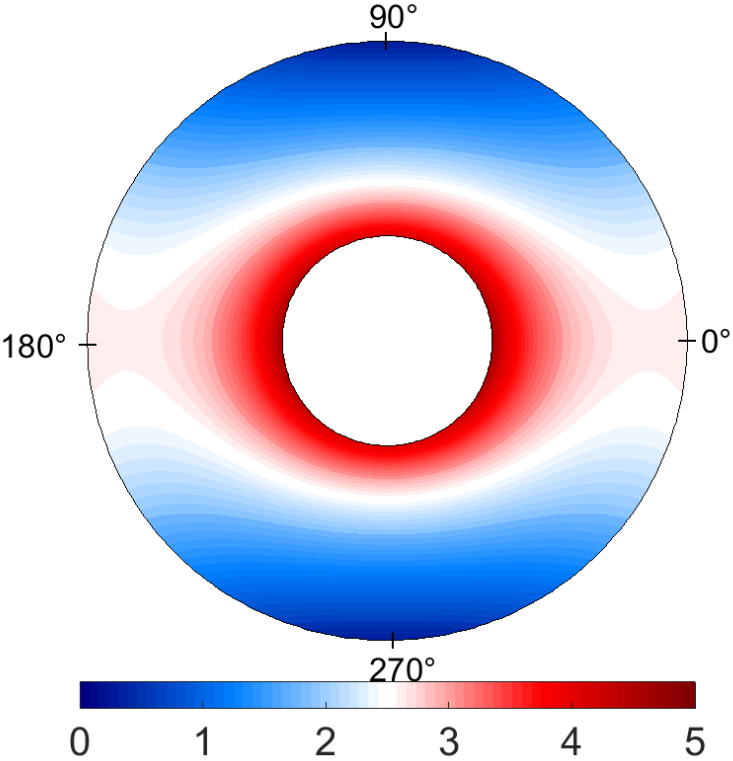
\includegraphics[width=0.9\textwidth]{sketches/equatorial_conductive.png}
  \caption*{(a) Equatorial view}
 \end{minipage}
 \hfill
 \begin{minipage}{0.62\textwidth}
  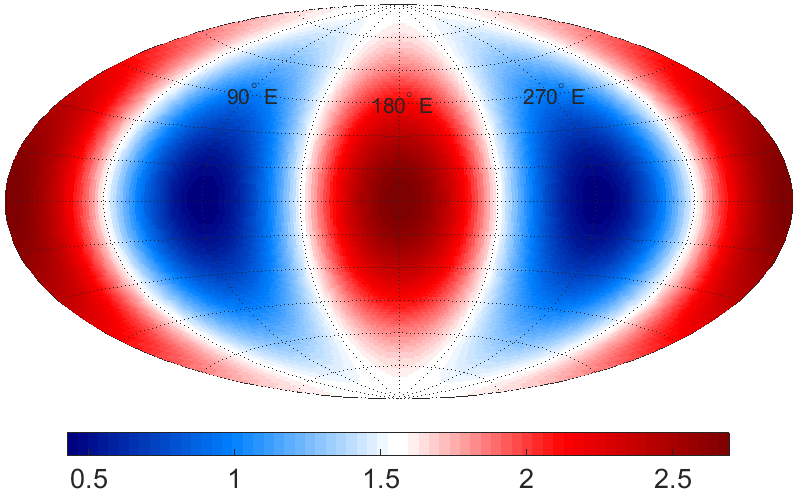
\includegraphics[width=0.9\textwidth]{sketches/surface_conductive.png}
  \caption*{(b) Surface projection}
 \end{minipage}
\caption{Conductive temperature field $T_\textrm{cond}$ in the equatorial plane (left) and as a \textit{Hammer-Aitov-projection} at the CMB (right) in a non dimensional form (see section \ref{sec:nondim}). The amplitude of the heat flux heterogeneity is $Amp_2^2 = 1$, heat flux maxima are located at 90$^\circ$ and 270$^\circ$, respectively. See Figure \ref{fig:fluxsketch} for a schematic overview. } 
\label{fig:conductives}
\end{figure}
\\
\\
The amplitude of heterogeneity, $Amp_2^2$, from now on referred to as $q^*$, plays a central role for the heat flux pattern. Figure \ref{fig:equator_flux} shows the core-mantle heat flux along the equator for two values of $q^*$. If the amplitude is chosen to be greater than 1, negative (inward) heat flux occurs in distinct regions around the heat flux minima. Heat flow from the mantle to the core produces gravitationally stable regions with respect to the temperature. Together with an always destabilizing compositional gradient, this can yield non-linear double-diffusive effects as fingering or layering. A scenario in which gravitationally stable regions play a role in core convection was recently discussed for Mercury \citep{tian2015magnetic}. Likewise for the Earth, where the heterogeneities in the core-mantle heat flux are generally considered to be rather mild \citep{aubert2008thermochemical, olson2002time, glatzmaier1999role}, \citet{nakagawa2008lateral} expect that heat locally flows from the mantle to the core where compositionally dense piles settle at the base of the mantle. Because of that and due to the fact that this study aims to explore the effect of a heat flux pattern on core convection from a general perspective, a relatively large value of $q^*\!=\!2$ is chosen in order to ensure a clearly discernible pattern effect. The choice of $q^* = 0$ refers to a uniform fixed flux boundary condition.
\begin{figure}[H]
 \begin{minipage}[left]{0.7\textwidth}
  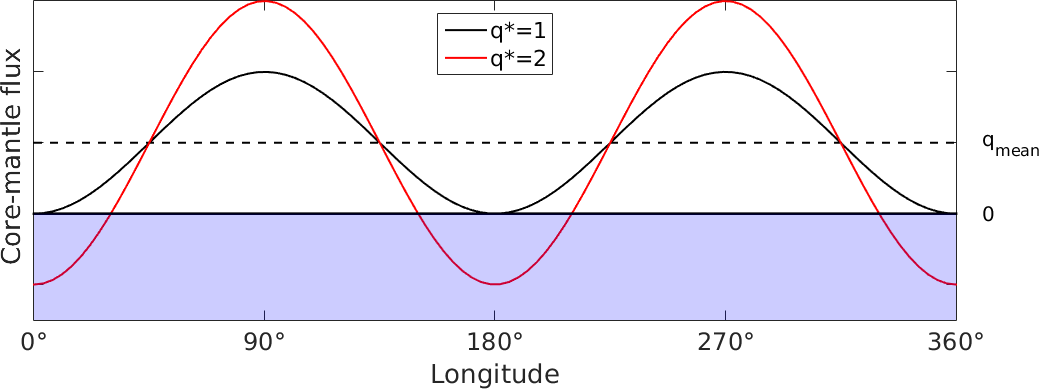
\includegraphics[width=1\textwidth]{sketches/eq_flux-trim.png}
\caption{Plot of the CMB - heat flux along the equator for amplitudes of heterogeneity $q^* = 1$ and $q^* = 2$. For $q^* > 1$, heat partially flows from the mantle to the core (blue region). } 
 \label{fig:equator_flux}
 \end{minipage}
 \hfill
  \begin{minipage}[right]{0.25\textwidth}
  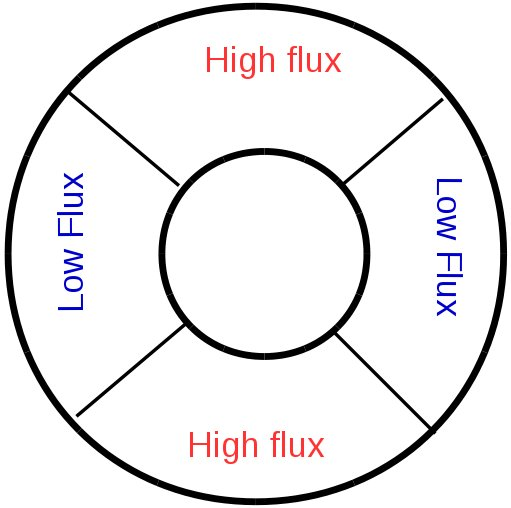
\includegraphics[width=0.92\textwidth]{sketches/pattern.jpg}
 \caption{Sketch of the equatorial plane and the distribution of high and low heat flux at the CMB. }
 \label{fig:fluxsketch}
  \end{minipage}
\end{figure}
\subsection{Non dimensional equations}
\label{sec:nondim}
A common procedure in fluid dynamics is to \textit{rescale} the equations introduced so far in order to reduce the number of parameters and to make the relevant physical processes intuitively more accessible. The new scales are adopted from \citet{trumper2012numerical}, they are summarized in table \ref{tab:scales}.
\begin{table}[H]
\centering
\begin{tabular}{ccc}
 Variable & Symbol & Scale\\
 \hline
 Length	& $\bm r$ & $D =R_o - R_i$\\
 Time	&$t$	  & $D^2/\nu$\\
 Velocity & $\bm u$ & $\nu / D$\\
 Temperature & $T$ & $ \beta D$\\
 Composition & $C$ & $\Delta C$ \\
 Pressure & $\pi$ & $\bar \rho \nu^2/D^2$\\
 Magnetic Field & $\bm B$ & $\sqrt{\eta \Omega \mu_0 \bar \rho}$\\
 \end{tabular}
 \caption{Overview of the the new scales that are introduced to non dimensionalize the magnetohydrodynamic system of equations that was introduced in the sections \ref{sec:continuity} to \ref{sec:boussinesq}.}
 \label{tab:scales} 
\end{table}
The application of these scales to equations \eqref{eq:incompressible}, \eqref{eq:force_balance3}, \eqref{eq:heat_equation}, \eqref{eq:chemical_equation} and \eqref{eq:induction} yields a system of non dimensional equations:
{\allowdisplaybreaks
\begin{subequations} \label{eq:nondim}
 \begin{align}
\label{eq:incompressible^}
{\bm {\hat \nabla}} \cdot \bm{ \hat u} = & \quad0, \\
\label{eq:momentum^} \nonumber
\frac{D \bm{ \hat u}}{D \hat t} = &- \bm{ \hat \nabla} \hat \pi' - \frac{2}{\textrm{Ek}}\, \bm{e_z} \times \bm{ \hat u} + \bm{ \hat \nabla}^2 \bm{ \hat u} + \frac{1}{\textrm{Ek}  \textrm{Pr}_\textrm{\tiny{m}}} \left( \bm{ \hat \nabla} \times \hat{ \bm B} \right) \times \hat{ \bm B}  \\ 
 &+ (\textrm{Ra}_\textrm{\tiny {T}} \hat{ T'} + \textrm{Ra}_\textrm{\tiny {C}} \hat{ C'} )(1-a) \hat{r} \, \bm{e_r}, \\
\label{eq:heat_equation^}
 \frac{D \hat T'}{D t} =& \quad \frac{1}{\textrm{Pr}_\textrm{\tiny T}} \bm{\hat \nabla}^2 \hat T',\\
 \label{eq:chemical_equation^}
 \frac{D \hat C'}{D t} =& \quad \frac{1}{\textrm{Pr}_\textrm{\tiny C}} \bm{\hat \nabla}^2 \hat C' \textrm{ and}\\
  \label{eq:induction^}
 \frac{\partial \bm {\hat{B}}}{\partial \hat t} = & \quad  \bm{\hat \nabla} \times (\bm{\hat u} \times \bm{\hat{B}}) + \frac{1}{\textrm{Pr}_\textrm{\tiny m}} \hat{ \bm \nabla}^2 \bm{\hat {B}}.
 \end{align}
\end{subequations}}\\
Nondimensional quantities are denoted by \^{} and they are related to their dimensional counterparts via $(\textrm{ }) = \textit{scale } \hat{(\textrm{ })}$. \\
The following parameters of similarity appear in the equations:
{\allowdisplaybreaks
 \begin{align}
\nonumber 
&\textrm{Thermal Rayleigh number : } &\textrm{Ra}_\textrm{\tiny {T}} = \frac{\alpha_\textrm{\tiny T} g \beta D^4}{\nu^2} \\ \nonumber 
%  \\ \nonumber 
&\textrm{Compositional Rayleigh number : } &\textrm{Ra}_\textrm{\tiny C} = \frac{\alpha_\textrm{\tiny C} g \Delta C D^3}{\nu^2} \\ \nonumber 
%  \\ \nonumber 
 &\textrm{Ekman number : }   & \textrm{Ek} = \frac{\nu}{\Omega D^2} \\ \nonumber 
%  \\ \nonumber 
&\textrm{Thermal Prandtl number : } & \textrm{Pr}_\textrm{T} = \frac{\nu}{\kappa_\textrm{T}} \\ \nonumber 
&\textrm{Compositional Prandtl number : } & \textrm{Pr}_\textrm{C} = \frac{\nu}{\kappa_\textrm{C}} \\ \nonumber 
&\textrm{Magnetic Prandtl number : } & \textrm{Pr}_\textrm{m} = \frac{\nu}{\eta} \\ \nonumber 
\end{align} 
}
The thermal and compositional Rayleigh numbers are measures for the vigor of convection due to thermal and compositional buoyancy forces, respectively. The definitions of $\textrm{Ra}_\textrm{\tiny {T}}$ and $\textrm{Ra}_\textrm{\tiny {C}}$ slightly differ because of the different scales chosen for temperature and composition (see table \ref{tab:scales}). $'\beta D'$ and $'\Delta C'$ refer to Neumann and Dirichlet type BCs for $T$ and $C$, respectively.  \\
Whether a fluid is constrained rather by rotation or viscosity is described via the Ekman number. \\
The distinction between a thermal and a compositional Prandtl number is a key feature of this study. It allows for differences in the dynamical response of the system to either thermally or compositionally dominated convective forcing. Roughly spoken, a large Prandtl number promotes viscous effects in a fluid, whereas a small one promotes inertia effects. The magnetic Prandtl number relates viscous and magnetic diffusion and therefore influences the amount of kinetic energy needed to sustain a magnetic field. \\
In the following, all $\hat{}$ will be omitted, since only non dimensional quantities are used.\\
The rescaled inner and outer radii of the spherical shell are R$_i = 0.539$ and R$_o = 1.539$, respectively.
\subsection{Conductive and convective fluctuations}
\label{sec:cond_conv}
The temperature field $T'$ and the compositional field $C'$, each reduced by the reference state fields $\bar T$ and $\bar C$, can be decomposed into a \textit{conductive part} which is the full solution if the system is subcritical and its \textit{convective perturbations} $\theta$ and $\zeta$:
\begin{equation*}
 T'(\bm r) = T_\textrm{cond}(\bm r) + \theta(\bm r) \quad \quad\quad C'(\bm r) = C_\textrm{cond}(\bm r) + \zeta(\bm r)
\end{equation*}
The stationary solutions $T_\textrm{cond}$ and $C_\textrm{cond}$ can be obtained analytically (see section \ref{sec:flux_pattern} for the temperature field), so that the numerical solution scheme needs to solve only for $\theta$ and $\zeta$. The conductive solution $C_\textrm{cond}$ follows from the stationary form of equation \eqref{eq:chemical_equation} and the BC described in section \ref{sec:bc}.
 The temperature and chemical equation transform to 
\begin{subequations} \label{cond_conv_heat_chem}
 \begin{align}
 \label{eq:theta}
 \frac{D \theta}{D t} = & \frac{1}{\textrm{Pr}_\textrm{T}} \bm \nabla^2 \theta - (\bm u \cdot \bm \nabla) T_\textrm{cond} \\
 \frac{D \zeta}{D t} = & \frac{1}{\textrm{Pr}_\textrm{C}} \bm \nabla^2 \zeta - (\bm u \cdot \bm \nabla) C_\textrm{cond},
\end{align}
\end{subequations}
if the decomposition is inserted. \\
\\
Furthermore, the equation of momentum slightly changes when temperature and composition are split into two parts.\\ 
$T_\textrm{cond}$ has a spherically symmetric and a spherically asymmetric part (see equation \eqref{eq:t_cond_cmb})
\begin{equation*}
T_\textrm{cond}(r,\vartheta,\phi) = t_0^0(r) + t_2^2(r,\vartheta,\phi),
\end{equation*}
where $t_0^0(r)$ is proportional to the constant $\mathcal{Y}_0^0$ and $t_2^2(r)$ to $\mathcal{Y}_2^2(\vartheta, \phi)$. \\
$t_0^0(r)$ and the spherically symmetric solution $C_\textrm{cond}(r)$ can be incorporated into the reduced pressure fluctuation term $\pi'$ via
\begin{equation*}
\pi = \pi' - (1-a)\left( \textrm{Ra}_\textrm{\tiny T} \int r\, t_0^0(r)\, dr + \textrm{Ra}_\textrm{\tiny C} \int r\, C_\textrm{cond}(r)\, dr \right).
\end{equation*}
Yet, it is not possible to find any potential $\varrho$ for the asymmetric part that satisfies 
\begin{equation*}
\bm \nabla \varrho = \textrm{Ra}_\textrm{\tiny T} \, t_2^2(r)(1-a) r \, \bm{e_r},
\end{equation*}
since this would demand $\partial \varrho/\partial \vartheta = \partial \varrho/\partial \phi = 0$, a condition that cannot be fulfilled by $t_2^2$ being a function of $\vartheta$ and $\phi$. Thus, $t^2_2$ appears in the buoyancy term of the momentum equation:
\begin{align}
\nonumber
 \frac{D \bm{ u}}{D  t} = &- \bm{  \nabla}  \pi - \frac{2}{\textrm{Ek}}\, \bm {e_z} \times \bm{  u} + \bm{  \nabla}^2 \bm{  u} + \frac{1}{\textrm{Ek}  \textrm{Pr}_\textrm{\tiny{m}}} \left( \bm{  \nabla} \times { \bm B} \right) \times { \bm B}  \\ 
 \label{eq:force_balance4}
 &+ (\textrm{Ra}_\textrm{\tiny {T}}  [\theta + t_2^2] + \textrm{Ra}_\textrm{\tiny {C}} { \zeta} )(1-a) {r} \, \bm{e_r}
\end{align}
\subsection{Thermal and chemical forcing}
\label{sec:thermal/chemical}
This work aims to explore the combined effect of the heat flux pattern at the CMB \textit{and} the thermo-chemical nature of the problem. Therefore, the system contains two distinct transport equations for temperature and composition (see section \ref{sec:internal_energy}). The buoyancy term in the equation of momentum \eqref{eq:force_balance4} consists of a thermal and a compositional part that are each controlled by one Rayleigh number, $\textrm{Ra}_\textrm{\tiny T}$ and $\textrm{Ra}_\textrm{\tiny C}$. In order to classify different scenarios according to the relative importance of the two driving mechanisms, \citet{breuer2010thermochemically} defined the \textit{fraction of thermal forcing}
\begin{equation}
\delta =  \frac{\textrm{Ra}_\textrm{\tiny T}}{\textrm{Ra}_\textrm{\tiny T} + \textrm{Ra}_\textrm{\tiny C}} = \frac{\textrm{Ra}_\textrm{\tiny T}}{\textrm{Ra}_\textrm{\tiny {total}}}
\end{equation}
for their model with isothermal and isochemical BCs. According to this definition, the end member cases with $\delta = 100\%$ and $\delta = 0\%$ are controlled exclusively by thermal and chemical forcing, respectively. Using this classification, one has to be aware that the choice of two different Prandtl numbers, $\textrm{Pr}_\textrm{T}$ and $\textrm{Pr}_\textrm{C}$, affects the critical Rayleigh numbers $\textrm{Ra}_\textrm{\tiny T}^\textrm{crit}$ and $\textrm{Ra}_\textrm{\tiny C}^\textrm{crit}$. The consequence is, that when keeping $\textrm{Ra}_\textrm{ total}$ fixed, the purely chemical case ($\delta = 0\%$) is to a higher degree super critical than the corresponding purely thermal case ($\delta = 100\%$) \citep{trumper2012numerical}. \\
In this model, Dirichlet type BCs are applied for the compositional and Neumann type BCs for temperature field (see section \ref{sec:bc}). Thus, 
\begin{equation}
 \textrm{Ra}_\textrm{\tiny C} = \frac{\alpha_\textrm{\tiny C} g \Delta C D^3}{\nu^2}
\end{equation}
is a \textit{classical Rayleigh number}, whereas 
\begin{equation}
 \textrm{Ra}_\textrm{\tiny {T}} = \frac{\alpha_\textrm{\tiny T} g \beta D^4}{\nu^2}
\end{equation}
contains the mean heat flux $\beta$ at the CMB and therefore is a \textit{flux Rayleigh number}. This has implications for the dynamics of the system \citep{kutzner2000effects} so that they can not be related to each other as directly as in the definition of $\delta$, mentioned above. Instead, the classification of the forcing will be made with respect to the particular \textit{supercriticalities} of the purely thermal and the purely compositional case, respectively. 
\begin{table}[H]
\centering
 \begin{tabular}{c c c}
  Ekman number& $\textrm{Ra}^\textrm{crit}_\textrm{\tiny T}$ (fixed flux) & $\textrm{Ra}^\textrm{crit}_\textrm{\tiny C}$ (isochemical) \\
  \hline
  $10^{-4}$& $ 51.2\times 10^4$ & $28.7 \times 10^4$\\
  $10^{-5}$& $ 108.7\times 10^5$ & $47.5 \times 10^5$\\
 \end{tabular}
\caption{Numerically determined critical Rayleigh numbers for the purely thermal and the purely chemical case with their distinct BCs. Two different Ekman numbers $\textrm{Ek} = 10^{-4}$ and $\textrm{Ek} = 10^{-5}$ are regarded.}
\label{tab:crit}
\end{table}
For each scenario with $\textrm{Ra}_\textrm{total} = \textrm{Ra}_\textrm{\tiny T} + \textrm{Ra}_\textrm{\tiny C} $, the individual supercriticalities $\gamma_\textrm{\tiny T} = \textrm{Ra}_\textrm{\tiny {T}} / \textrm{Ra}_\textrm{\tiny T}^\textrm{crit}$ and $\gamma_\textrm{\tiny C} = \textrm{Ra}_\textrm{\tiny {C}} / \textrm{Ra}_\textrm{\tiny C}^\textrm{crit}$ of the thermal and the chemical forcing are computed according to table \ref{tab:crit}. The relative thermal supercriticality $\delta^*$, then reads
\begin{equation}
\label{eq:delta_new}
 \delta^* := \frac{\gamma_\textrm{\tiny T}}{\gamma_\textrm{\tiny T}+ \gamma_\textrm{\tiny C}} = \frac{\gamma_\textrm{\tiny T}}{\gamma_\textrm{total}}.
\end{equation}
The relative thermal supercriticality will be used in the following study to characterize a thermo-chemical forcing scenario. The end member cases $\delta^*=100\%$ and $\delta^*=0\%$ refer to purely thermal and purely compositional driving, respectively. \\ \par \noindent
Due to the limited time available for this work, critical Rayleigh numbers are computed only for the non-magnetic case. Thus, the classification of the dynamo cases in section \ref{sec:dynamo} will be made according to these, too. This is not correct for the reason that the presence of a magnetic field can affect the onset of convection \citep{chandrasekhar1970hydrodynamic}. 
\subsection{Numerical method}
\label{sec:numerics}
The study makes use of the code PARODY \citep{dormy1997modelisation, dormy1998mhd} in a version that was extended by a compositional component in order to simulate double-diffusive forcing \citep{trumper2012numerical}. \\
The velocity field and the magnetic field can both be represented in terms of their scalar toroidal and poloidal potentials, since they are solenoidal. This reduces the amount of unknown variables by two and implicitly respects the equation of continuity ($\bm \nabla \cdot \bm u = 0$) and the fact that no magnetic monopoles exist ($\bm \nabla \cdot \bm B = 0$). The poloidal-toroidal decomposition reads
\begin{equation}
\label{eq:poltor_u}
 \bm u = \bm \nabla \times \bm \nabla \times (u_p \, \bm r) + \bm \nabla\times (u_t \, \bm r)
\end{equation}
for the velocity field and 
\begin{equation}
\label{eq:poltor_B}
 \bm B = \bm \nabla \times \bm \nabla \times (B_p \, \bm r) + \bm \nabla\times (B_t \, \bm r)
\end{equation}
for the magnetic field, where the subscript $t$ denotes the toroidal and $p$ the poloidal part. The equation of momentum \eqref{eq:force_balance4} can be reformulated according to \eqref{eq:poltor_u} and the induction equation \eqref{eq:induction^} according to \eqref{eq:poltor_B}, whereas the heat equation \eqref{eq:heat_equation^} and the compositional equation \eqref{eq:chemical_equation^} do not transform under the decomposition. For a detailed description of the resulting system of equations, the reader is referred to the work of \citet{dormy1997modelisation} and \citet{trumper2014thermo}. \\ \par
A common next step is to choose a spectral representation of all variables in order to profit from the special geometry of the problem. \citet{glatzmaier1995three} and \citet{kuang1997earth} already made use of a a spherical harmonics expansion in the numerical solution schemes for their early dynamo models. A variable in PARODY, represented by $f(r,\vartheta,\phi)$, is expanded in spherical harmonics according to
\begin{equation}
 f(r,\vartheta,\phi) = \sum\limits_{l=0}^{\infty} \sum \limits_{m=0}^l \, f_l^m(r) \, \mathcal{Y}_l^m(\vartheta,\phi)
\end{equation} 
and the equations described in the previous sections are solved in the spectral domain. This simplifies the computation of lateral derivatives immensely. Only the non-linear terms appearing are calculated in the physical space and re-transformed to the spectral domain before entering the solution scheme. This is why the method is called \textit{pseudospectral}. \\
In the radial direction, the numerical scheme makes use of a second order finite difference discretization. The grid is refined at the boundaries in order to resolve small scale boundary effects properly.\\ A combination of an implicit and an explicit method is applied for the time integration. With the help of an implicit Crank-Nicolson scheme, the diffusion terms are integrated, whereas an explicit Adams-Bashforth method is used for the non-linear and force terms.\\ \par \noindent 
The spectral resolution follows a criteria by \citet{christensen1999numerical} according to which the power spectra of all quantities computed drops by at least two orders of magnitude between the highest and the lowest spectral degree. \\ \par \noindent
As initial condition for all cases shown here, zero velocity and a small perturbation in all modes of the temperature and compositional field are used. In the magnetic cases, an additional perturbation is applied to the toroidal as well as the poloidal part of the magnetic field. A more detailed description can be found in \citet{trumper2014thermo}.
\subsection{Diagnostics}
\label{sec:diagnostics}
This chapter briefly introduces the diagnostic quantities and techniques that are used in the course of this work:\\ \par
\begin{itemize}
 \item[-] \textbf{Vorticity}\\
 The vorticity $\bm \omega$ describes the local rotation of a fluid and can be computed via the curl of the velocity:
 \begin{equation}
 \bm \omega = \bm \nabla \times \bm u
\end{equation}
 \item[-] \textbf{Helicity}\\
 Helicity is generated where a flow $\bm u$ is oriented parallel to its vorticity vector $\bm \omega$. It can be computed by the dot product
 \begin{equation}
  \mathcal{H} = \bm u \cdot \bm \omega
 \end{equation}
\item[-] \textbf{Reynolds number and magnetic Reynolds number}\\
 The Reynolds number $Re$ and the magnetic Reynolds number $Re_m$ measure the ratio of inertia to viscous and magnetic diffusion in the fluid, respectively. They are defined via a typical flow velocity that is the rms-velocity in this case:
 \begin{equation}
 \textrm{Re} = \frac{D\,u_\textrm{rms}}{\nu}\quad\quad \textrm{     and    } \quad\quad \textrm{Re}_m = \frac{D\, u_\textrm{rms}}{\eta}
 \end{equation}\noindent 
   \item[-] \textbf{Elsasser number}\\
 The Elsasser number $\Lambda$ compares the importance of the Lorentz force to that of the Coriolis force in a magnetohydrodynamic problem. As the scaling of the magnetic field includes the rotation rate $\Omega$, $\Lambda$ can be easily computed by
 \begin{equation}
  \Lambda = \langle \bm B^2 \rangle_{r,\vartheta,\phi},
 \end{equation}
where $\langle \quad \rangle$ is an averaging operator.
 \item[-] \textbf{Relative dipole strength}\\
 Only the first twelve spectral degrees of the relative strength of the magnetic dipole at the CMB are measurable for the geomagnetic field because of the filtering effect of the overlying mantle. Therefore, the relative dipole strength $f_\textrm{dip}$ is defined as the ratio of the rms axial dipole component to the total rms field up to the harmonic degree $l=12$. 
 \end{itemize}

\newpage

\section{Thermo-chemical core convection}
\label{sec:thermo-chemical}
The $\mathcal{Y}_2^2$ temperature BC at the CMB introduces an inherent axial asymmetry to the system that is visible in the flow field as well as in the temperature and compositional field. This section aims to point out the most important characteristics that are typical of non-magnetic convection under the influence of the new BC. Therefore, the focus lies on the heat flux pattern and thus on the thermal driving, not on the \textit{dual}-forcing mechanism. Nevertheless, one thermo-chemical case will be discussed in the following. It will be seen that the heterogeneous thermal BC strongly affects the distribution of the light component. \\ \par \noindent
A key feature of the non homogeneous model is the formation of stationary vortex columns that are attached to lateral temperature variations in the lower-most mantle. The aim of this section is to explain their formation and their meaning for the system.\\
In the beginning, sections \ref{sec:onset}, \ref{sec:vortex_clolumns} and \ref{sec:thermal_wind} provide the theoretical background for the explanation and interpretation of the results.
As a start, the \textit{onset of convection in the uniform case} in form of an azimuthally drifting Rossby wave will be briefly discussed in section \ref{sec:onset}. The solution to the uniform BC scenario inhibits \textit{columns of constant vorticity} that will be the topic of section \ref{sec:vortex_clolumns}. Although this section still deals with the uniform case, its results can be applied to the heterogeneous system. Section \ref{sec:thermal_wind} introduces the reader to the \textit{geostrophic and the thermo-chemical wind balance}. Especially the latter plays an important role here, because it considers lateral density gradients which are emphasized by the laterally varying heat flux condition. \\
In section \ref{sec:radial_flow} the theoretical concepts described in the preceding sections are applied to the numerical data for a non homogeneous case in order to explain the structure of the flow field in the equatorial plane. A relation derived from the thermo-chemical wind balance serves well as an explanation for the distribution of radial up- and downwellings in the equatorial plane and therefore makes the structure of the flow field understandable.\\ 
The interplay of azimuthal and radial velocity creates a vorticity pattern that is locked to the heat flux heterogeneities imposed by the mantle. Section \ref{sec:attached_columns} shows and interprets the stationary vortex columns that originate in the equatorial plane but elongate through the whole sphere due to the geostrophic constraint that promotes vertically invariant structures (see section \ref{sec:thermal_wind}). In this context, some implications for the compositional field will be discussed.\\
Section \ref{sec:temp_field} describes the long-term averaged temperature field that evolves under the influence of the heat flux pattern and is meant to allow the reader a better idea of the scenario.\\ \par \noindent
Throughout this section, the Prandtl numbers will be held fixed at $\textrm{Pr}_\textrm{\tiny T} = 3$ and $\textrm{Pr}_\textrm{\tiny C} = 0.3$, the Ekman number at $\textrm{Ek} = 10^{-4}$.\\
The influence of the heat flux BC can best be observed in temporal averages \citep{olson2002time}. Consequently, all data that is shown in this section refers to such averages. The averages are taken in the statistically stationary state.\\

\subsection{The onset of convection in the uniform case}
\label{sec:onset}
In a rotating system that is homogeneously forced, convection sets in in the form of a thermal Rossby wave \citep{busse1970thermal, busse2002convective}. The rotation imposes a column like structure to the system that is aligned with the axis of rotation ($z$-axis, see Figure \ref{fig:sketch_busse}) and drifts in azimuthal direction. This rotational constraint will be described in terms of the \textit{Taylor-Proudman theorem} in section \ref{sec:thermal_wind}. Within the present set of parameters, the columns lie adjacent to the \textit{tangential cylinder} (TC), a cylindrical surface that touches the inner core at the equator. \citet{busse2002convective} describes a mean flow instability that leads to differential rotation (the variation of azimuthal velocity with radius, in the following referred to as DR), evolving under the influence of a spherical geometry. Differential rotation presumably plays a central role in the magnetic field generation as it is an ingredient for the $\omega$-effect \citep{roberts2007theory}. \\ \par \noindent
\begin{figure}[t]
 \begin{minipage}[]{0.46\textwidth}
 \centering
 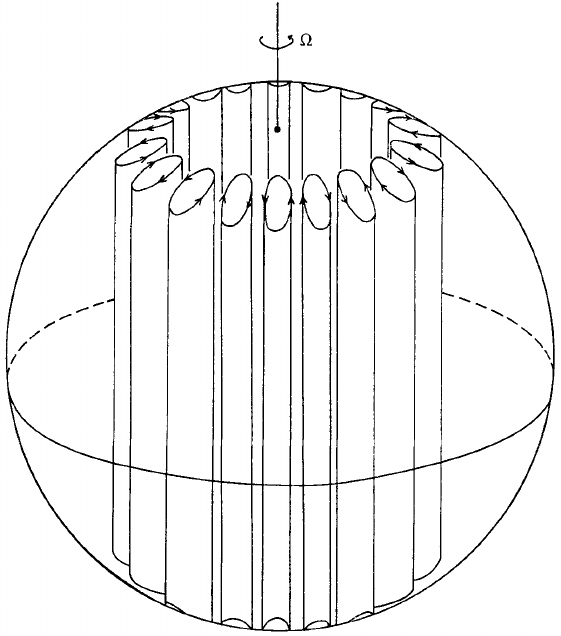
\includegraphics[width=1.05\textwidth]{sketches/busse_1975_onset.png}
 \caption{Sketch of the onset of convection for a rotating spherical shell. Convection columns form adjacent to the TC (figure changed after \citet{busse1970thermal}). The columns can be visualized by different quantities. Here, they are sketched as contours of constant vorticity.}
 \label{fig:sketch_busse}
\end{minipage}
\hfill
\begin{minipage}[]{0.47\textwidth}
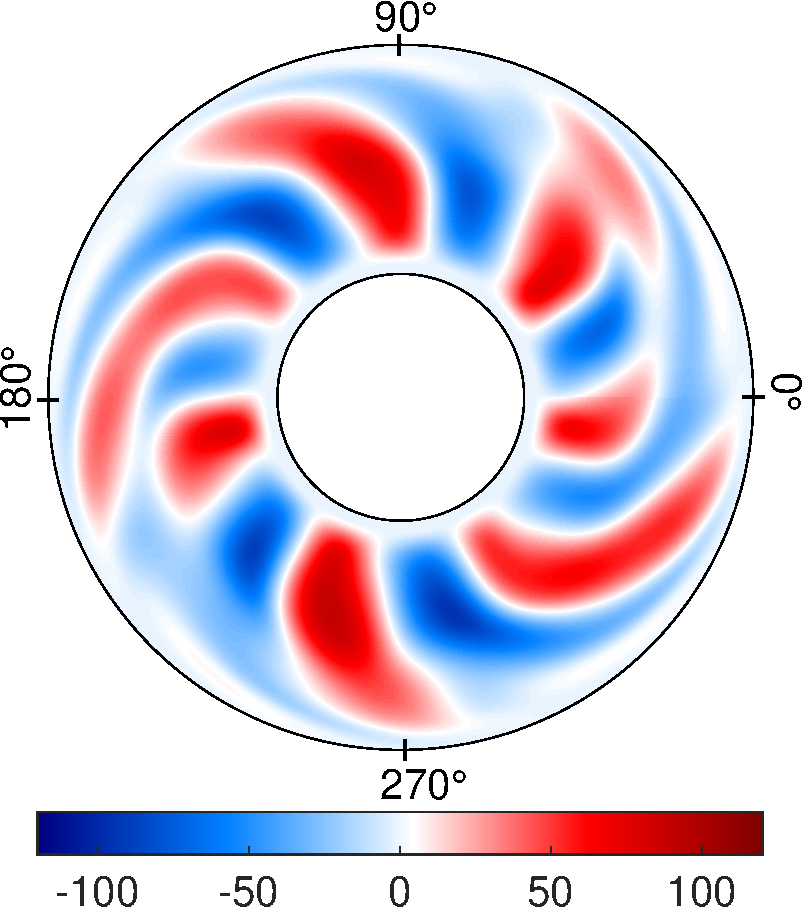
\includegraphics[width=\textwidth]{graphs/iso_440_ex_rad-crop.pdf}
\caption{Snapshot of the radial velocity in the equatorial plane (view from the north pole, like all other equatorial views in the following) for a uniform case with  $\textrm{Ra}_\textrm{\tiny T} = \textrm{Ra}_\textrm{total} = 4.4\times 10^6$, $\textrm{Pr}_\textrm{\tiny T} = 0.3$, $\textrm{Ek}=10^{-4}$ and $q^* = 0$. The convection columns are tilted and slightly deformed compared to Figure \ref{fig:sketch_busse}. }
\label{fig:radial_vel_ex}
\end{minipage}
\end{figure} \noindent
According to the analytical theories of \citet{jones2000onset} and \citet{dormy2004onset}, the azimuthal length scale of each convection column would be extremely small in case of the Earth's rotation rate. Therefore, this scenario is assumed to be unrealistic and the dominance of rotation as compared to buoyancy is questioned. The alternative is a rather three-dimensional, turbulent regime \citep{king2009boundary}, for which, on the other hand, the mechanism of the magnetic field production is an open question.
\subsection{Columns of constant vorticity}
\label{sec:vortex_clolumns}
As mentioned above, convection in rapidly rotating systems is organized in a column like structure at onset \citep{busse1970thermal}. The question whether this structure is maintained, even in the highly supercritical LOC, has important implications for the understanding of the geodynamo.\\ 
Since the first findings of self sustained dynamos \citep{glatzmaier1995three, kuang1997earth}, different kinds of dynamo \textit{processes} have been discussed. Hence, the circular transformation between poloidal and toroidal magnetic field is a necessary ingredient for all of them \citep{roberts2007theory}. The \textit{vortex columns}, visualized in Figures \ref{fig:sketch_busse} and \ref{fig:vort_uniform}, are important sources of \textit{helicity} and therefore necessary for the macrospcopic $\alpha$-effect, that can transform either poloidal to toroidal field or vice versa \citep{roberts2007theory,jones2011planetary}. For a detailed explanation of the $\alpha$-effect and its importance for the geodynamo, the reader is referred to the literature cited above. For the moment it suffices to know that helicity is a key quantity in the discussion of dynamo action. \\
This section aims to explain the mechanism of helicity production inside of vortex columns. \\ \par \noindent
Although motion parallel to the $z$-axis is strongly constrained by rotation (see equation \eqref{eq:geostrophy2}), the spherical form of the boundaries necessarily relaxes this constraint locally and vertical flow is unavoidable \citep{busse2002convective, gillet2006quasi}. An important example for the relaxation of the Taylor-Proudman theorem in this context is the \textit{secondary circulation} inside of vortex columns \citep{olson1999numerical, aubert2008magnetic, christensen2011geodynamo}, sketched in Figure \ref{fig:secondary_circulation}.\\
\textit{Ekman pumping} and \textit{suction} are boundary layer effects that are distinct to systems with no-slip conditions (as in this study, see section \ref{sec:bc}). They evolve due to the interplay between the rotation dominated bulk and the viscosity dominated Ekman layer. In \textit{cyclones}, i.e., vortex columns with positive vorticity $\omega > 0$, Ekman pumping induces a vertical flux away from the CMB towards the equator. Ekman suction causes motion towards the CMB in \textit{anticyclones}, where $\omega < 0$. Although both mechanisms take place in the boundary layers, they potentially induce vertical motion in the whole column. A more detailed description can be found in \citet{pedlosky2013geophysical}.\\
The variation of buoyancy along the $z$-axis inside of a vortex column acts as a second source of vertical motion \citep{olson1999numerical}. As in the case of Ekman suction and pumping, this motion is oriented equatorwards in cyclones and away from the equator in anticyclones. It is independent of the viscous BCs and therefore it makes this discussion applicable to a wider range of model configurations. 
\begin{figure}[H]
 \begin{minipage}[left]{0.53\textwidth}
  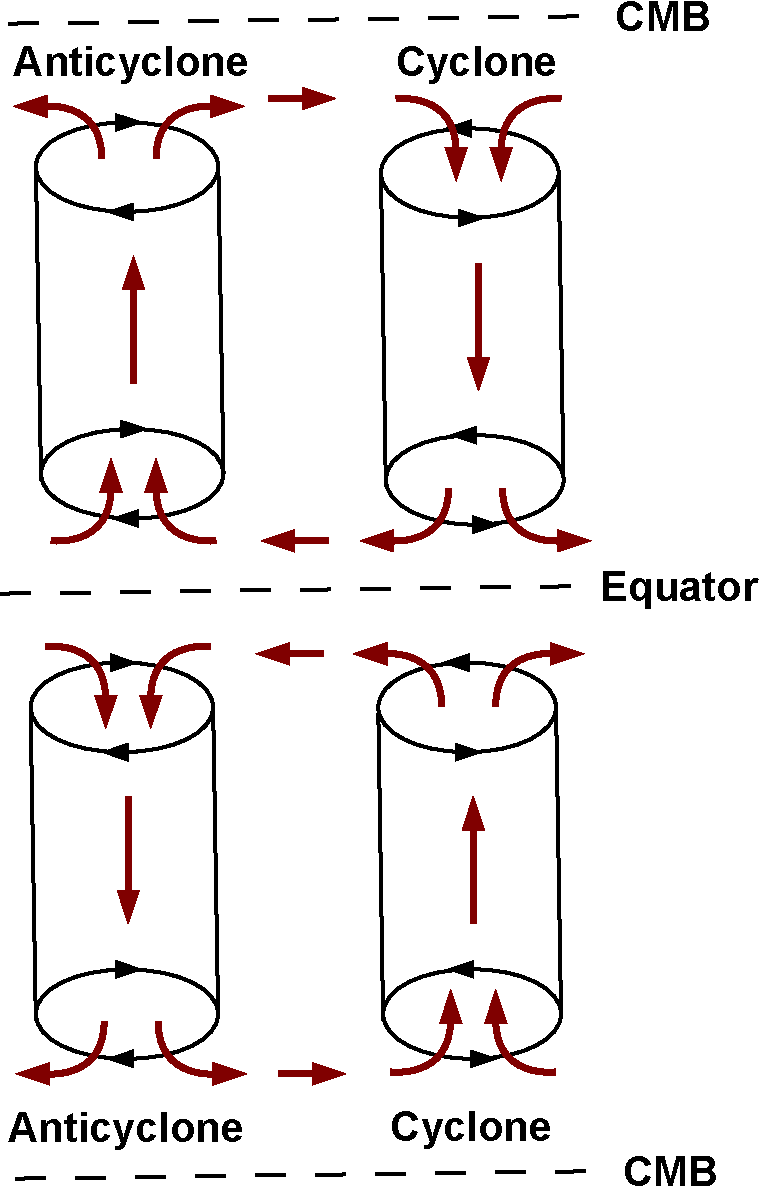
\includegraphics[width =  \textwidth]{sketches/secondary_circulation-crop.pdf}
  \caption{Sketch of the secondary circulation induced by a pair of a cyclonic and an anticyclonic vortex. The two convection columns can be imagined as part of the sketch in Figure \ref{fig:sketch_busse}, a situation typical for the onset of convection.}
  \label{fig:secondary_circulation}
 \end{minipage}
\hfill
\begin{minipage}[right]{0.42\textwidth}
Figure \ref{fig:secondary_circulation} shows a sketch of the secondary circulation. A cyclone (with flow \textit{towards} the equator in the northern and southern hemisphere), causes a divergent flow at the equator, whereas an anticyclone (with flow away from the equator) acts converging at the equator. The opposite is true near the CMB. A cyclone and an anticyclone together form a \textit{circular} motion that superimposes the primary vortical motion. The interaction of a vorticity carrying fluid column and a vertical flow produces helicity $\mathcal{H}$. \\ \par \noindent
The role of \textit{converging} and \textit{diverging} flow at the CMB plays a distinct role in the framework of this study. Converging flows tend to collect magnetic field lines in their vicinity, whereas a diverging flow acts expelling \citep{aubert2008magnetic, jones2011planetary}. This will be further discussed in section \ref{sec:dynamo}. The effect of the secondary circulation on the compositional field can be observed in section \ref{sec:attached_columns}.
\end{minipage}
\end{figure} \noindent

\subsection{The geostrophic and the thermo-chemical wind balance}
\label{sec:thermal_wind}
The rotation rate of the LOC, measured in terms of the inverse of the non dimensional Ekman number $\textrm{Ek}^{-1}$, is very high (see table \ref{tab:parameter}). The \textit{Rossby number} $Ro = \frac{\mathcal{U}}{\Omega \mathcal{L}}$ quantifies the relative importance of the inertia force compared to the Coriolis force in the equation of momentum. If it is small, a system is predominantly rotationally constrained and this suggests simplifications, accordingly. The inertia term drops out and viscosity can be neglected as well, due to $\textrm{Ek} = \frac{\nu}{\Omega D^2} \ll 1$. In the absence of gravitational instabilities, this yields the \textit{geostrophic balance}
\begin{equation}
\label{eq:geostrophy}
 -\frac{2}{\textrm{Ek}}\bm{e_z} \times \bm u= \bm \nabla \pi,
\end{equation}
where the rotational force is balanced by the pressure gradient \citep{vallis2006atmospheric, jones2007thermal}. The \textit{Taylor-Proudman theorem} follows from equation \eqref{eq:geostrophy}, if the curl is applied:
\begin{equation}
\label{eq:geostrophy2}
 (\bm{e_z} \cdot \bm \nabla) \bm u = 0.
\end{equation}
It states that variations in the velocity field parallel to the axis of rotation ($z$-axis) are suppressed. The system tends to take on a two dimensional solution, although this is never realizable in a sphere which naturally has sloping boundaries \citep{busse2002convective}.\\
Relation \eqref{eq:geostrophy} slightly changes, if buoyancy forces due to temperature or compositional variations cannot be neglected. The \textit{thermo-chemical wind balance} then describes, how lateral gradients in $T$ and $C$ cause flow gradients parallel to the axis of rotation \citep{jones2007thermal}: 
\begin{align}
 \label{eq:thermal_wind}
-2 \frac{\partial \bm u}{\partial z}= (1-a) \textrm{Ek}\,\bm \nabla \times \left( \textrm{Ra}_\textrm{\tiny T}(\theta + t_2^2) + \textrm{Ra}_\textrm{\tiny C}\zeta \right)\bm r.
%=& \quad  (1-a) \textrm{Ek}\textrm{Ra}_\textrm{\tiny T}\left( \frac{1}{\textrm{} \vartheta}\frac{\partial (\theta + t_2^2)}{\partial \phi}\, \bm{e_\vartheta} + \frac{\partial (\theta + t_2^2)}{\partial \vartheta}\, \bm{e_\phi} \right)
\end{align}
This equation is obtained when adding the buoyancy term from equation \eqref{eq:force_balance4} to the force balance \eqref{eq:geostrophy} and taking the curl again. Equation \eqref{eq:thermal_wind} will be important in the following, because the conductive response to the heat flux pattern, $t_2^2$, prescribes lateral temperature gradients to the system. Additionally, dynamical variations $\theta$ and $\zeta$, especially along the polar coordinate $\vartheta$, are assumed to drive thermo-chemical winds in the sphere \citep{trumper2012numerical}. 
\subsection{The formation of radial flux patches by azimuthal temperature gradients in the equatorial plane}
\label{sec:radial_flow}
The non-axisymmetric distribution of up- and downwellings in the time-averaged flow is a feature that is distinct to non homogeneous forcing provided by the heterogeneous core-mantle heat flux. \citet{zhang1992convection} and \citet{dietrich2016core} analytically show that the azimuthal position of in- and outward radial motion in the equatorial plane is determined by the azimuthal temperature gradient $\partial T / \partial \phi$. \\
Equation \eqref{eq:thermal_wind} is used as a starting point, whereupon only thermal forcing is regarded ($\textrm{Ra}_\textrm{\tiny C} = 0$). Since the $z$-axis plays a central role in the geostrophic context, cylindrical coordinates are used with $s$ as a radial distance from the axis of rotation. According to \citet{dietrich2016core}, the velocity field is split into a geostrophic part $\bm u^g$ and an ageostrophic part $\bm u^a$ with $\bm u = \bm u^g(s,\phi) + \bm u^a(s,z,\phi)$, where the geostrophic part per definition is independent of the $z$-position. To compute the geostrophic flow, the $z$-average of the $z$-component of equation \eqref{eq:thermal_wind} is needed,
\begin{equation}
\label{eq:wind_z1}
-2\,\Big \langle \frac{\partial u_z}{\partial z} \Big \rangle_z = {(1-a)\textrm{Ek}\textrm{Ra}_\textrm{\tiny T}} \, \langle \bm{e_z} \cdot \bm \nabla \times (\theta + t_2^2) \bm r \rangle_z,
\end{equation}
where the average of a function $f$ can be computed by
\begin{equation*}
 \langle f \rangle_z (s,\phi) = \frac{1}{2H} \int_{-H}^{+H} f(s,z,\phi) \, dz,
\end{equation*}
with $H = \sqrt{R_o^2 + s^2}$ as the half height of a cylinder at the radial position $s$ \citep{gillet2006quasi}. The right-hand-side (rhs) of equation \eqref{eq:wind_z1} can be transformed to (now in spherical coordinates)
\begin{equation}
\label{eq:wind_z2}
 \textrm{rhs} = {(1-a)\textrm{Ek}\textrm{Ra}_\textrm{\tiny T}} \, \bigg \langle \bm{e_z} \cdot \left( \frac{1}{\textrm{sin}\vartheta} \frac{\partial}{\partial \phi}(\theta + t^2_2)\, \bm{e_\vartheta} - \frac{\partial}{\partial \vartheta} (\theta + t^2_2) \, \bm{e_\phi} \right) \bigg \rangle_z
\end{equation}
The conductive temperature profile $t_2^2$ is symmetric with respect to the equator, hence its lateral gradient antisymmetric and it drops out when averaged over the $z$-axis. The temperature variation $\theta$ is likely to be distributed equatorial symmetric as well and therefore it is neglected, likewise. In cylindrical coordinates, equation \eqref{eq:wind_z2} now reads
\begin{equation}
\label{eq:wind_z3}
 \textrm{rhs} = (1-a) \textrm{Ek}\textrm{Ra}_\textrm{\tiny T} \frac{1}{s} \bigg \langle \frac{\partial}{\partial \phi} (\theta + t^2_2) \bm{e_z} \cdot \bm{e_\vartheta} \bigg \rangle_z.
\end{equation}
Following \citet{gillet2006quasi}, the left-hand-side of equation \eqref{eq:wind_z1} transforms to
\begin{equation}
\label{eq:wind_z4}
-2\,\Big \langle \frac{\partial u_z}{\partial z} \Big \rangle_z = -\frac{1}{H} \int_{-H}^{+H} \frac{\partial u_z}{\partial z} \, dz = -\left( - u_s^g \, \frac{2s}{H^2} \right).
\end{equation}
The slope of the spherical boundary is responsible for the fact, that a radial velocity component enters the $z$-averaged equation in order to balance the effect of the boundary shape.\\
In the equatorial plane, $\bm{e_z}\cdot \bm{e_\vartheta} = -1$, $r=s$ and the radial velocity $ u_s^g$ in cylindrical coordinates equals the radial velocity $u_r^g$ in spherical coordinates. It can now be expressed in terms of the azimuthal temperature gradient:
\begin{equation}
 \label{eq:ugr}
 u_r^g = -\frac{H^2}{2r^2}(1-a)\textrm{Ek}\textrm{Ra}_\textrm{\tiny T} \,\bigg \langle \frac{\partial}{\partial \phi}(\theta + t^2_2) \bigg \rangle_z.
\end{equation}
The position of the maximum (minimum) azimuthal temperature gradient should thus coincide with radial downwellings (upwellings) (see relation \eqref{eq:ugr} that contains a minus sign) in the equatorial plane. Since only the $z$-averaged / geostrophic  part of the velocity field $\bm u$ contains radial components (\citep{dietrich2016core}, $u_r^g$ is the full radial flow in this approximation. \\ \par \noindent
\begin{figure}[t]
 \centering
 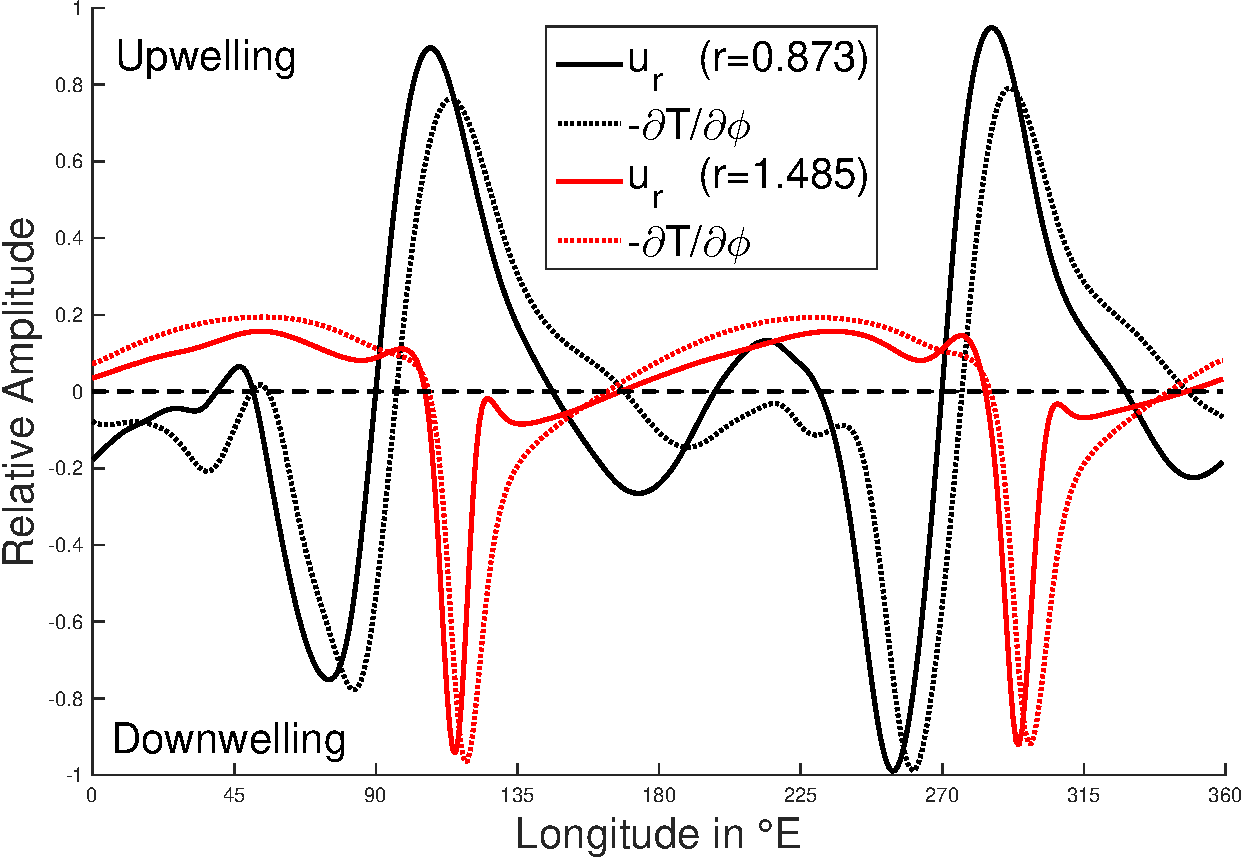
\includegraphics[width=\textwidth]{graphs/q2_200_ur_dTp-crop.pdf}
 \caption{Azimuthal profiles of the radial velocity $u_r$ (solid lines) and the negative azimuthal temperature gradient $-\partial (\theta + t_2^2)/\partial \phi$, here referred to as $-\partial T/\partial \phi$ (dotted lines), at mid depth (black, $r=0.873$) and at the top of the free stream near the CMB (red, $r=1.485$), normalized with respect to their individual maximum value. All values are measured in the equatorial plane. As parameters, $\textrm{Ra}_\textrm{\tiny T} = \textrm{Ra}_\textrm{total} = 2\times 10^6$ and $q^* = 2$ are used besides the Prandtl and Ekman number as mentioned above.}
\label{fig:ur_dTp}
 \end{figure} \noindent
Figure \ref{fig:ur_dTp} shows two azimuthal profiles of the the radial velocity $u_r$ (solid lines) and the negative azimuthal temperature gradient $\partial (\theta + t^2_2) / \partial \phi$ (dotted lines) in the equatorial plane. One is taken at mid depth (black lines), the other one on top of the free stream, i.e., right under the viscous boundary layer, near the CMB (red lines). All values are normalized with respect to their maxima in order to make them comparable in one plot.\\ 
The forcing in this case is purely thermal with a Rayleigh number $\textrm{Ra}_\textrm{\tiny T} = \textrm{Ra}_\textrm{total} = 2\times 10^6$ that is slightly supercritical: $\textrm{Ra}_\textrm{\tiny T} \approx 3.9 \times \textrm{Ra}_\textrm{crit}$ (see table \ref{tab:crit}). \\ \par \noindent
It becomes clear that the $\phi$-gradient of the temperature serves well as an explanation for the location of the two radial downwellings near the CMB. The two negative extrema of the radial velocity coincide nearly perfectly with the maxima of the azimuthal temperature gradient. Only the small kinks in front of and behind the extrema of $u_r$ cannot be explained by $\partial (\theta + t_2^2)/\partial \phi$ in this first order approach.\\ 
In a purely conductive regime with $\textrm{Ra}_\textrm{\tiny T} < \textrm{Ra}_\textrm{crit}$, the maxima of $\partial (\theta + t_2^2) / \partial \phi = \partial t_2^2 / \partial \phi$ (because $\theta=0$ in the subcritical case) would be located $45^\circ$ E of the heat flux maxima (located at $90^\circ$ E and $270^\circ$ E, see Figure \ref{fig:conductives} for the conductive temperature field) \citep{zhang1992convection}. The fact that the phase shift is only $30^\circ$ here (see Figure \ref{fig:ur_dTp}) can be attributed to the supercriticality of this case. More specifically, the azimuthal velocity field is responsible for the westward shift of the downwelling because it inhibits strong retrograde flow near the CMB around $135^\circ$ E (see Figure \ref{fig:equatorial_vel_temp}(c)). \\ \par \noindent
\begin{figure}[t]
\centering
\begin{minipage}[left]{0.32\textwidth}
   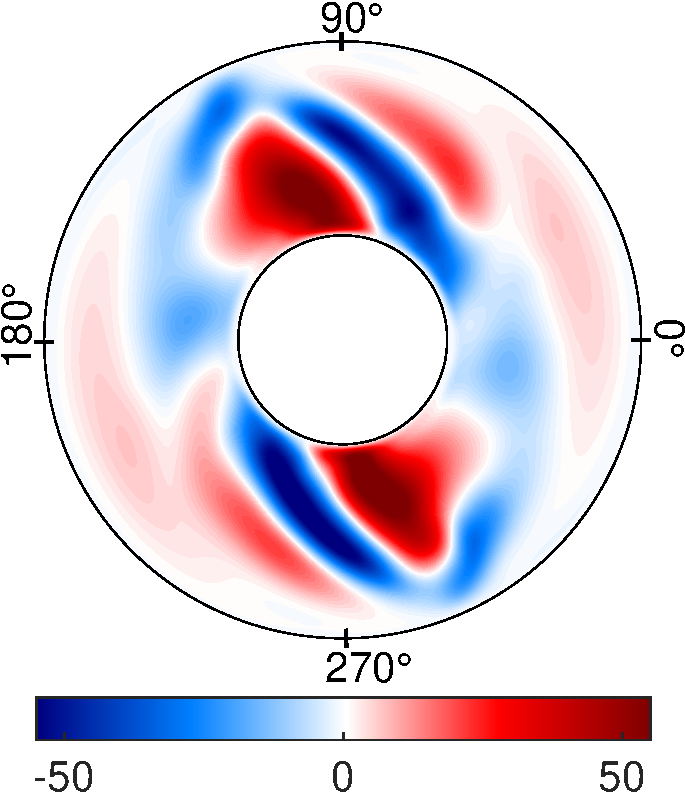
\includegraphics[width = \textwidth]{graphs/q2_200_d080_rad-crop.pdf}
   \caption*{(a) Radial Velocity}
\end{minipage}
\hfill
\begin{minipage}[center]{0.32\textwidth}
   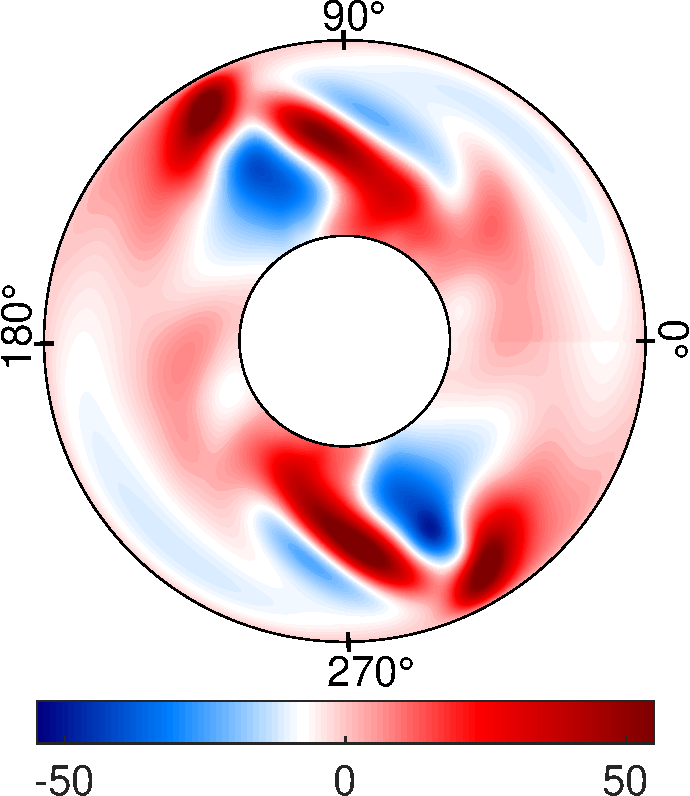
\includegraphics[width = \textwidth]{graphs/q2_200_dTp-crop.pdf}
   \caption*{(b) $\partial T / \partial \phi$, rescaled}
\end{minipage}
\hfill
\begin{minipage}[right]{0.32\textwidth}
    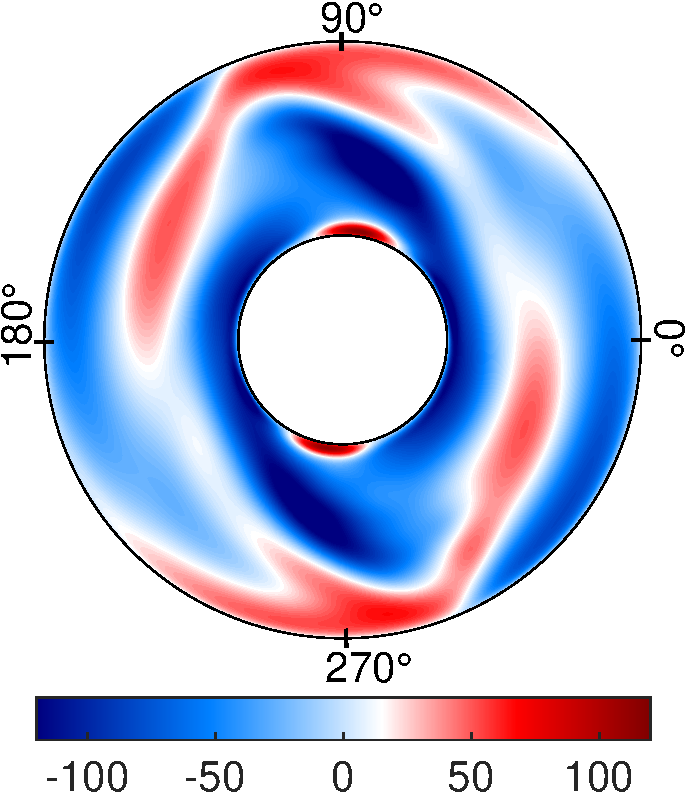
\includegraphics[width = \textwidth]{graphs/q2_200_d080_az-crop.pdf}
  \caption*{(c) Azimuthal velocity}
\end{minipage}
\caption{Equatorial contours of (a) the radial velocity, (b) the azimuthal temperature gradient $\partial (\theta + t_2^2) /\partial \phi$ and (c) the azimuthal velocity. The values in (b) are rescaled according to equation \eqref{eq:ugr} (without the minus sign) in order to be comparable to (a). The case is the same as in Figure \ref{fig:ur_dTp}. }
\label{fig:equatorial_vel_temp}
\end{figure} \noindent
In the outer region of the core, the two downwellings (around 120$^\circ$ and 300$^\circ$ E) are more pronounced than the complementary upwellings (around 45$^\circ$ and 225$^\circ$ E, see Figures \ref{fig:ur_dTp} and \ref{fig:equatorial_vel_temp}(a)). \citet{dietrich2016core} explain this asymmetry with the azimuthal part of the non-linear temperature advection term $-\frac{\partial \theta}{\partial \phi}u_\phi$ (see equation \eqref{eq:theta} that promotes positive azimuthal temperature gradients and therefore downwellings at the corresponding longitudes.  \\ \par \noindent
The radial flow in the deeper regions of the core (e.g. the solid black line Figure \ref{fig:ur_dTp}) has a more complex form and is thus not as directly as in the upper layers related to the $\mathcal{Y}_2^2$ heat flux pattern. Broad and pronounced upwellings develop right under the CMB downwellings at $\sim110^\circ$E and $\sim290^\circ$E. They are also visible in the temperature field in Figure \ref{fig:flowfield_temp} in form of hot plumes. \\
The downwellings observed at the CMB bend in jet-like structures in retrograde direction towards the ICB (see Figure \ref{fig:equatorial_vel_temp}(a)). The bending happens due to strong zonal westward flows at mid depth at $\sim 90^\circ$E and $\sim 270^\circ$E, respectively (see Figure \ref{fig:equatorial_vel_temp}(c)).  \\ 
Although the flow structure in the deeper core regions is more complex than at the CMB, equation \eqref{eq:ugr} and therefore the thermo-chemical wind relation provide a good explanation for the radial flow field (compare Figure \ref{fig:equatorial_vel_temp}(a) and (b)). \\ \par
\begin{figure}[t]
 \centering
 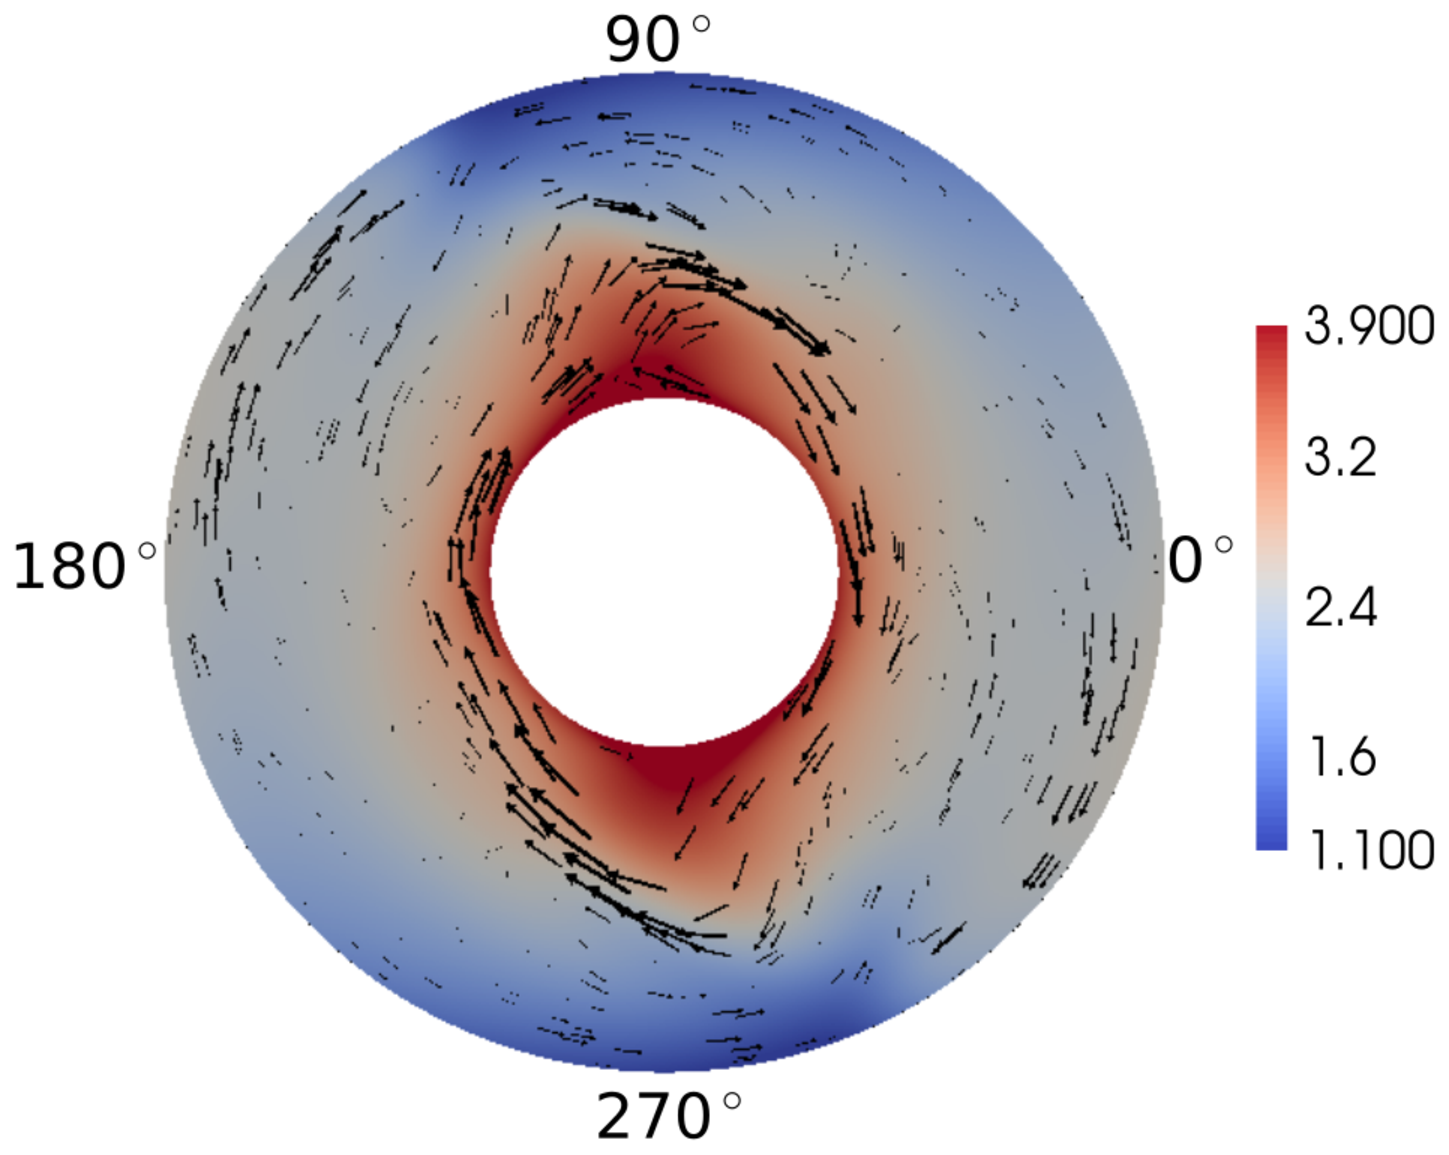
\includegraphics[scale=0.5]{graphs/q2_200_temp_vel-crop2.pdf}
 \caption{Horizontal velocity vectors in the equatorial plane, scaled by the corresponding flow magnitude. The background contour shows the full non dimensional temperature field $ T = \theta + T_\textrm{cond}$. The two strong upwelling plumes at the ICB (at $\sim 110^\circ$E and $\sim 290^\circ$E) and the bending jet-like downwellings right above are clearly visible.}
\label{fig:flowfield_temp}
 \end{figure} \noindent
The azimuthal flow in the equatorial plane is, in reaction to the radial flow, convergent (divergent) in the neighborhood of downwellings (upwellings). This can be observed either in the horizontal flow field (Figure \ref{fig:flowfield_temp}) or in the radial and azimuthal flow fields (Figure \ref{fig:equatorial_vel_temp}(a) and (c)). In order to preserve mass conservation, a downwelling attracts azimuthal flow whereas an upwelling rather expels fluid particles and therefore causes azimuthally diverging flow.
\subsection{Stationary vortex columns attached to mantle heterogeneities}
\label{sec:attached_columns}
The well structured Rossby wave solution is perturbed, if heterogeneous heat flux conditions are applied at the CMB. Nevertheless, columns of constant vorticity play an important role in the solution. The long-term averaged data bears a non-axisymmetric vorticity pattern that can be related to the geometry of the CMB heat flux. This pattern contains \textit{stationary vortex columns} elongated through the whole sphere parallel to the axis of rotation. In contrast to that, all uniform cases (e.g. the snapshot in Figure \ref{fig:vort_uniform}) yield axisymmetric distributions of vorticity in long-term averages because the Rossby wave solution constantly moves in azimuthal direction \citep{busse2002convective}. \\
\begin{figure}[t]
\begin{minipage}[left]{0.47\textwidth}
 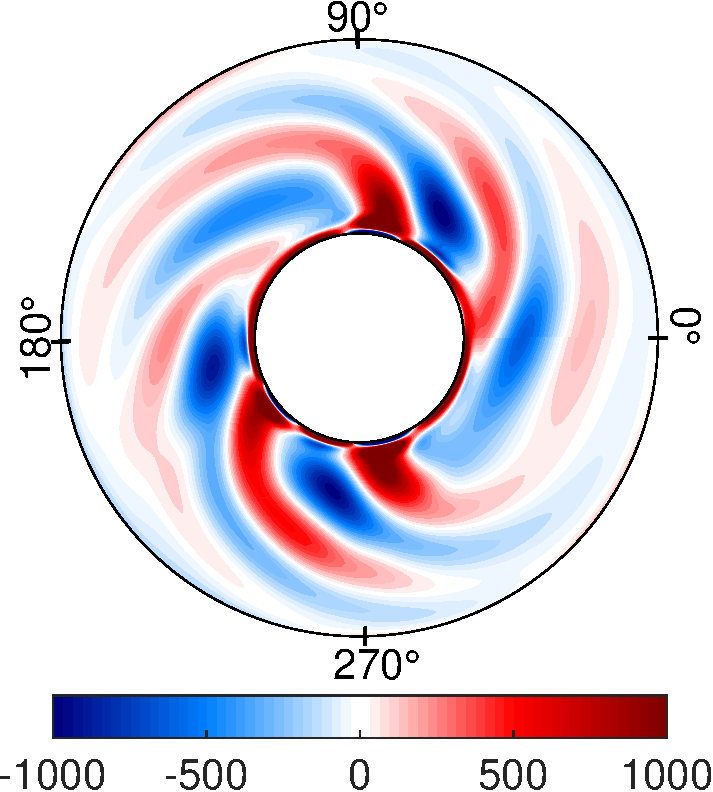
\includegraphics[width =\textwidth]{graphs/vorticity/q0_100_ex_vort-crop.pdf}
 \caption{Snapshot of the $z$-component of vorticity in the equatorial plane for a slightly supercritical, uniform case: $\textrm{Ra}_\textrm{\tiny T} = 10^{6}$.  }
 \label{fig:vort_uniform}
\end{minipage}
\hfill
\begin{minipage}[right]{0.47\textwidth}
 \includegraphics[width=0.96\textwidth]{graphs/vorticity/q2_200_d080_vort-crop.pdf}
 \caption{Long-term averaged equatorial contour of the $z$-vorticity for the same case as described in Figure \ref{fig:equatorial_vel_temp}. The vorticity in the boundary layers is not resolved.}
 \label{fig:q2_200_d080_vort}
\end{minipage}
\end{figure} \noindent
The secondary circulation, which was described in section \ref{sec:vortex_clolumns}, is expected to have an effect on the flow that can be localized at a fixed position in the spherical shell, it is \textit{locked} to the mantle \citep{gibbons2000convection}. \\ \par \noindent
The interaction of the azimuthal and the radial velocity field in the equatorial plane (Figure \ref{fig:equatorial_vel_temp}(a) and (b)) yields the vorticity distribution that is shown in Figure \ref{fig:q2_200_d080_vort}. Tilted patches of strong negative vorticity close to the ICB lie beneath prograde jets of positive vorticity right under the heat flux maxima at $90^\circ$E and $270^\circ$E. Additionally, a band of negative vorticity is located between $90^\circ$ and $180^\circ$E and between $270^\circ$ and $360^\circ$E. \\
\begin{figure}[t]
 \centering
 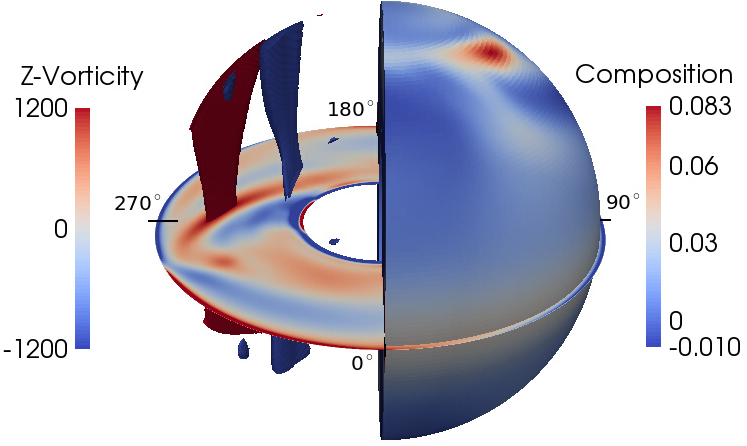
\includegraphics[scale = 0.7]{graphs/vorticity/q2_200_vort.png}
 \caption{\textbf{Left hemisphere}: $z$-component of the vorticity in the equatorial plane (see Figure \ref{fig:q2_200_d080_vort}) and contour surfaces at $\omega_z = -1200$ (blue) and $\omega_z = 1200$ (red). \textbf{Right hemisphere}: Compositional perturbation $\zeta$ close to the CMB at $ r = 1.5$. As parameters, $\textrm{Ra}_\textrm{total}=  2\times 10^6$, $\delta = 95\%$ and $q^* = 2$ are chosen.}
 \label{fig:vort_chem}
\end{figure} \noindent
In Figure \ref{fig:vort_chem}, the long-term averaged vorticity distribution of a thermo-chemically driven case is shown in the left hemisphere, whereas the right hemisphere depicts the compositional perturbation $\zeta$. The forcing is composed of a thermal and a chemical origin, with a mild portion of 5\% uniform compositional forcing ($\delta^*=95\%$)). The total Rayleigh number remains $\sim 4$ times supercritical in order to be comparable to the previous case. The vorticity contours in the left hemisphere yield the stationary vortex columns attached to the heat flux maxima mentioned above, as in the previous cases. An anticyclone (blue) elongates close to the TC from the northern to the southern CMB. A cyclonic column (red) lies parallel to the anticyclone in the radially outward direction. The two vorticity columns visible in the left hemisphere likewise exist in the left hemisphere (see the symmetry in the vorticity distribution in figure \ref{fig:q2_200_d080_vort}). Here, the compositional perturbation yields a maximum at the intersection of the blue anticyclone with the CMB and a deficit when going towards the equator in lateral direction, i.e., where the red cyclone intersects the CMB. \\
The excess and deficit composition results from the divergent and convergent flow at the peak of the anticyclone and the cyclone, respectively. The corresponding mechanism is sketched in Figure \ref{fig:secondary_circulation}. The vertical upward flow inside the anticyclone successively transports compositionally enriched material from the ICB (equator) towards the CMB and produces a local compositional maximum there. For the cyclone, the process works the other way round but since the cyclones are less dominant than the anticyclonic columns, the compositional minima are also less pronounced than the maxima.\\
In the present scenario, the compositional forcing rather acts as 'tracer' that visualizes the vertical transport from the ICB, where the chemical component is released, to the CMB. A portion of 5 \% compositional forcing is expected to have only a little effect on the dynamics of the system compared to the purely thermal case from above. Nevertheless, the principal behavior described in this section is not restricted to those cases with only a minor degree of compositional forcing. Patches of compositionally enriched fluid near the CMB can be found even in scenarios with $\delta^* = 12 \%$, i.e., only a small degree of thermal forcing. The above mechanism is thus expected to be persistent over a wide range of $\delta^*$. \\
The observation made here has implications for the inner core (a) as well as for the structure of the CMB (b). (a) The extraction of compositionally enriched material from the inner core is amplified at the intersection between anticyclones and the ICB (due to the convergent flow there, see figure \ref{fig:secondary_circulation}). \citet{aubert2008thermochemical} states that such a mechanism could enhance the inner core growth locally. (b) The successive dynamical accumulation of compositionally enriched material in certain regions near the CMB, visible in figure \ref{fig:vort_chem}, may lead to a saturation and a herewith connected sedimentation of the originally soluted light element. \\ \par \noindent
The compositional field shown in the right hemisphere of figure \ref{fig:q2_200_d080_vort} provides evidence that divergent and convergent flow near the CMB can be localized at fixed positions at the spherical surface. The ability of convergent flows to concentrate magnetic field lines and thereby intensify the field locally was discussed by several authors \citep{olson1999numerical, aubert2008magnetic, jones2011planetary}. In section \ref{sec:dynamo}, the reverse effect of expulsion of magnetic field lines by divergent flow will be important as well. Above all, it is important to mention that the flow properties found in this section can not be transferred directly to the dynamo case because of the action of the Lorentz force.
\subsection{The effect of the flux pattern on the temperature field}
\label{sec:temp_field}
Figure \ref{fig:q2_200_temp}(a) shows the same equatorial view on the temperature field as Figure \ref{fig:flowfield_temp} in section \ref{sec:radial_flow}. The color map was slightly rescaled to make the phase shift between the temperature maxima at the CMB at $\sim 170^\circ$ and $\sim 350^\circ$ and the heat flux maxima (at $\sim 90^\circ$ and $\sim 270^\circ$) visible. The phase shift originates in the flow field and can be explained by the observations made in the previous chapter: Strong radial motion occurs predominantly in the region under the heat flux maxima. The up- and downwellings visible in Figure \ref{fig:flowfield_temp} intensify the cooling mechanism, thus go along with a colder core region. The hot regions coincide with strong azimuthal motion along the CMB that inhibits the transport of heat out of the core. \\ \par \noindent
The surface projection of the temperature field at the CMB (Figure \ref{fig:q2_200_temp}(b)) confirms that the temperature field in the slightly supercritical case is nearly a phase shifted version of the conductive temperature field (Figure \ref{fig:conductives}(b)) \citep{zhang1992convection}. 
\begin{figure}[b!]
 \begin{minipage}[left]{0.33\textwidth}
  \centering
  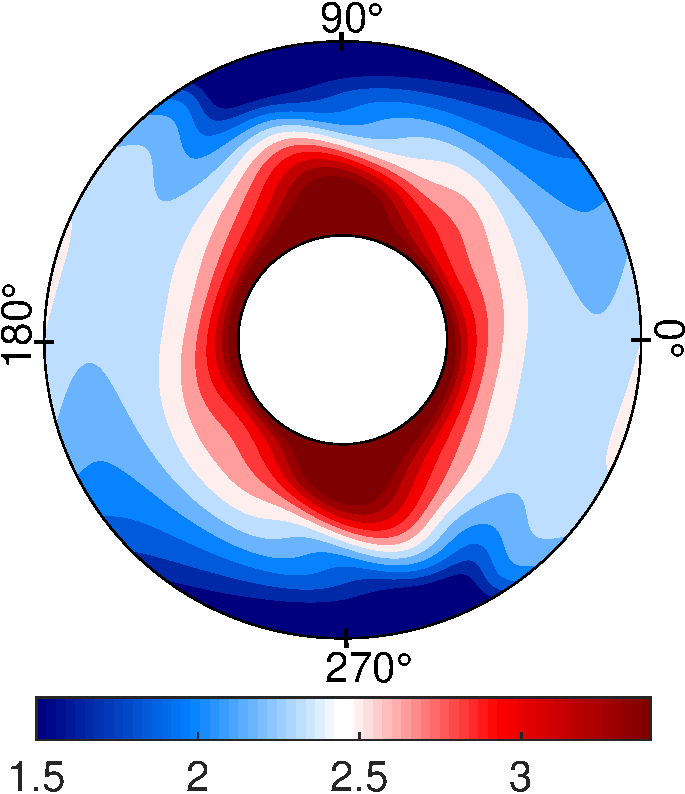
\includegraphics[width=\textwidth]{graphs/q2_200_eq_temp_field2-crop.pdf}
  \caption*{(a) Equatorial plane}
 \end{minipage}
 \hfill
\begin{minipage}[right]{0.63\textwidth}
 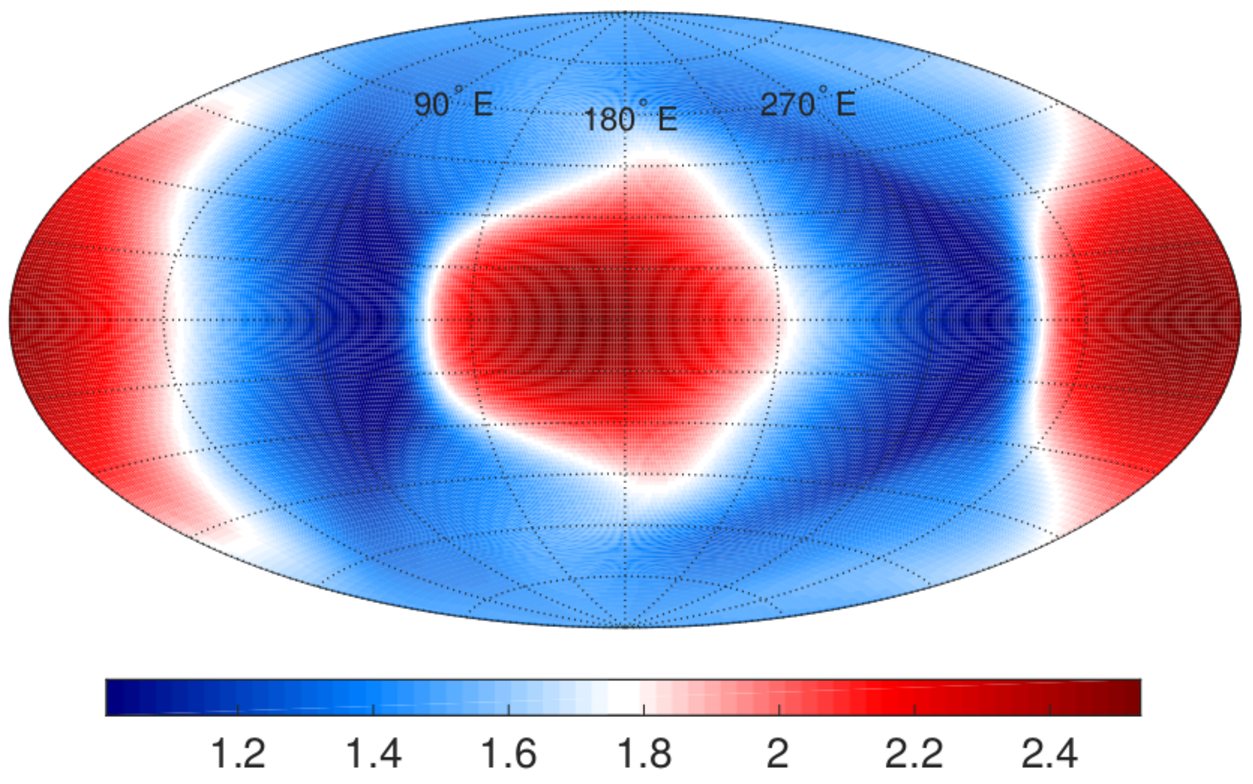
\includegraphics[width=\textwidth]{graphs/q2_200_tammer-crop.pdf}
 \caption*{(b) Surface projection at the CMB}
\end{minipage}
\caption{Full temperature field $ T = \theta + T_\textrm{cond}$ for the same case as above in (a) the equatorial plane and (b) as a surface projection right under the CMB at r = 1.485. (a) is the same graph as in Figure \ref{fig:flowfield_temp}, but the color map is 'shortened' in order to pronounce the phase shift of the temperature field. }
\label{fig:q2_200_temp}
\end{figure} \noindent

\newpage

\section{Thermo-chemical dynamo action}
\label{sec:dynamo}
\begin{figure}[b!]
 \begin{minipage}{0.13\textwidth}
 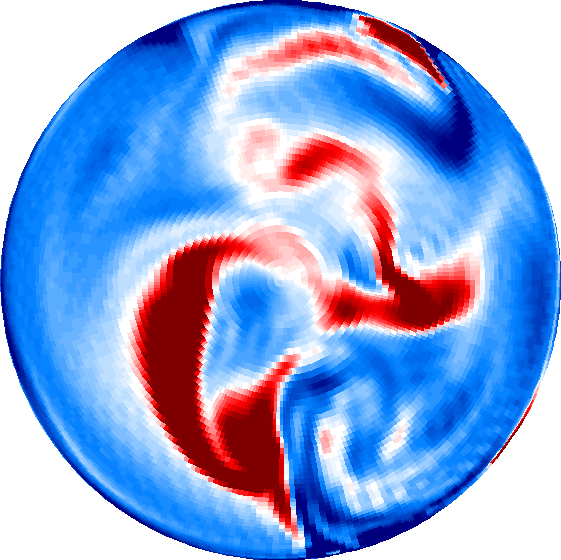
\includegraphics[width=\textwidth]{graphs/dynamo/snapshots/G_trim-0.png} \\
 \vfill
 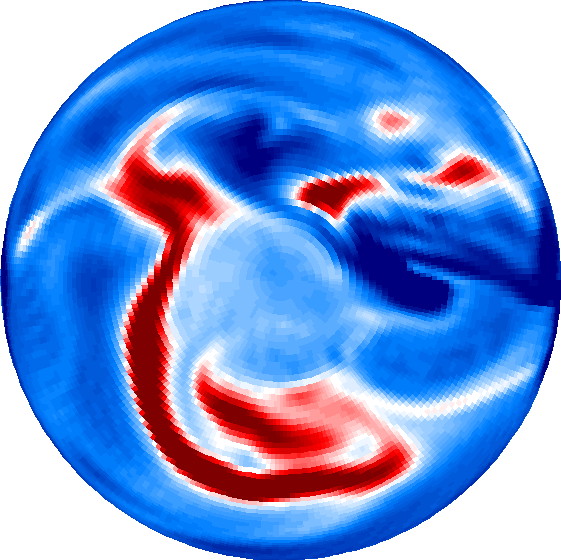
\includegraphics[width=\textwidth]{graphs/dynamo/snapshots2/G_trim-1.png}
 \end{minipage}
\hfill
  \begin{minipage}{0.13\textwidth}
 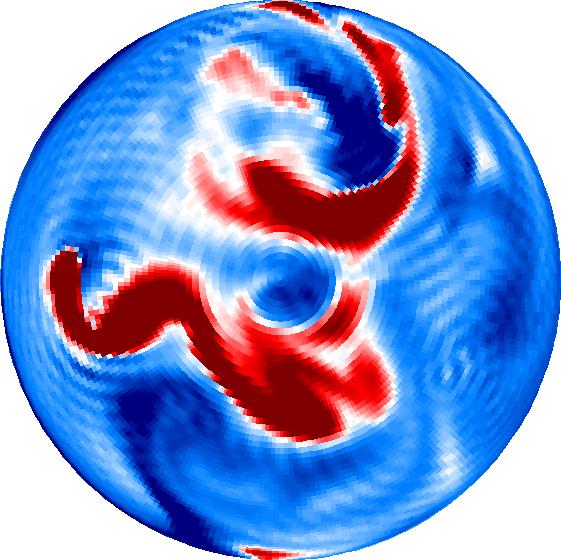
\includegraphics[width=\textwidth]{graphs/dynamo/snapshots/G_trim-1.png}\\
  \vfill
  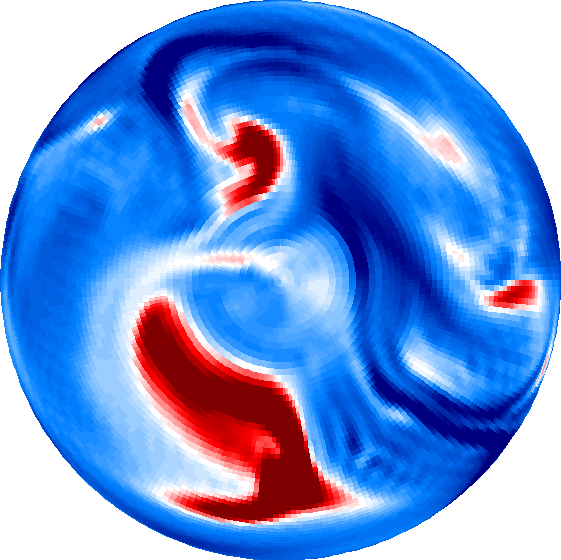
\includegraphics[width=\textwidth]{graphs/dynamo/snapshots2/G_trim-2.png}
 \end{minipage}
 \hfill
  \begin{minipage}{0.13\textwidth}
 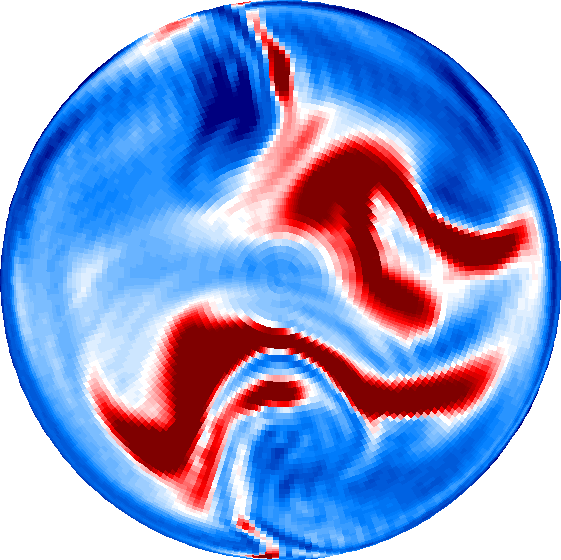
\includegraphics[width=\textwidth]{graphs/dynamo/snapshots/G-trim-27.png}\\
 \vfill
  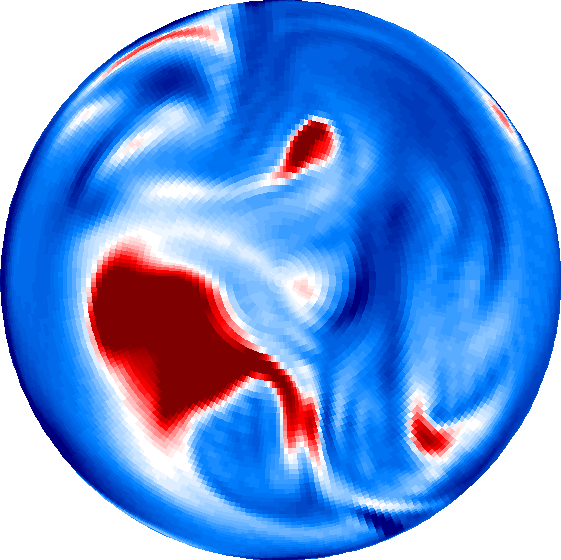
\includegraphics[width=\textwidth]{graphs/dynamo/snapshots2/G_trim-3.png}
 \end{minipage}
 \hfill
  \begin{minipage}{0.13\textwidth}
 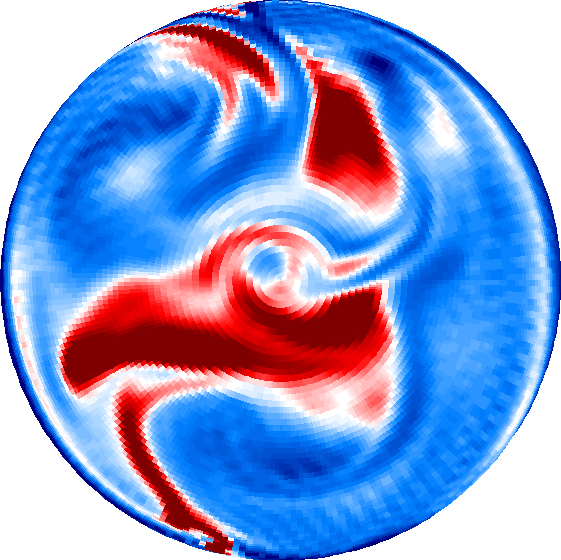
\includegraphics[width=\textwidth]{graphs/dynamo/snapshots/G_trim-3.png}\\
 \vfill
  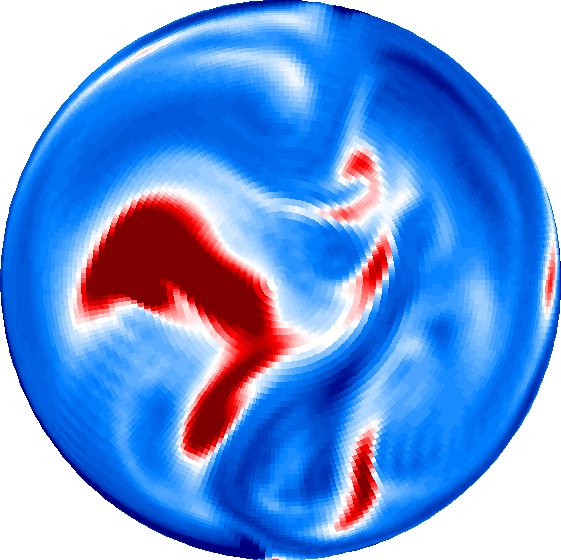
\includegraphics[width=\textwidth]{graphs/dynamo/snapshots2/G_trim-4.png}
 \end{minipage}
 \hfill
  \begin{minipage}{0.13\textwidth}
 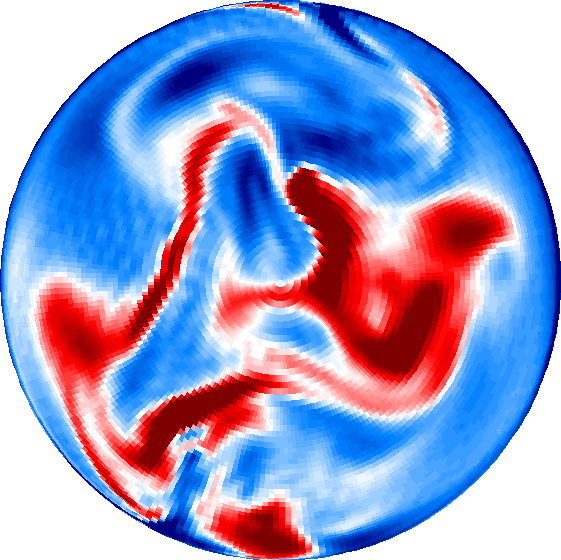
\includegraphics[width=\textwidth]{graphs/dynamo/snapshots/G_trim-4.png}\\
 \vfill
  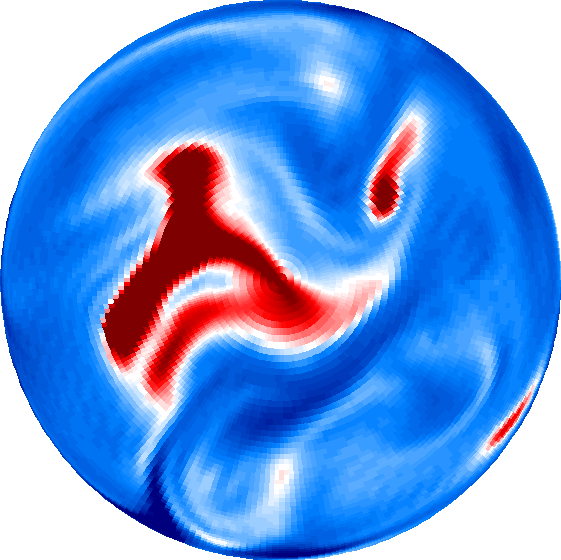
\includegraphics[width=\textwidth]{graphs/dynamo/snapshots2/G_trim-5.png}
 \end{minipage}
\hfill
  \begin{minipage}{0.13\textwidth}
 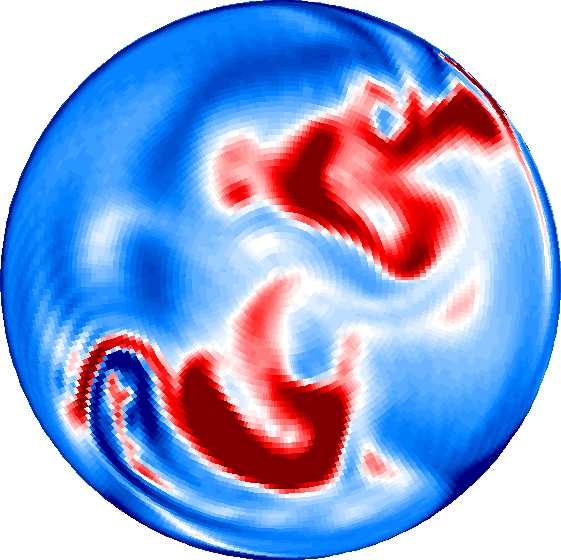
\includegraphics[width=\textwidth]{graphs/dynamo/snapshots/G_trim-12.png}\\
 \vfill
  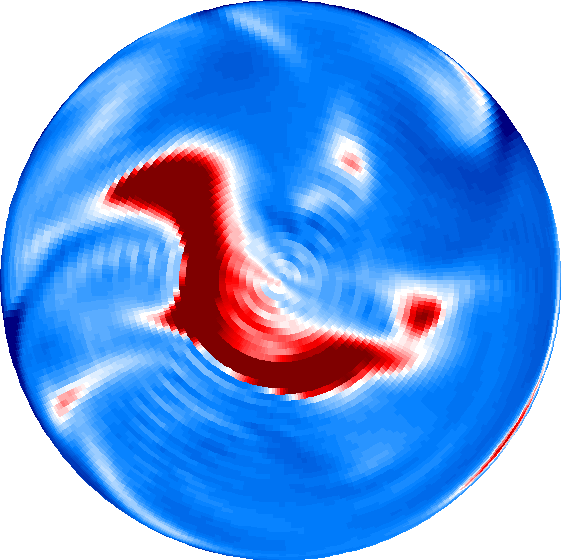
\includegraphics[width=\textwidth]{graphs/dynamo/snapshots2/G_trim-8.png}
 \end{minipage}
\hfill
  \begin{minipage}{0.16\textwidth}
 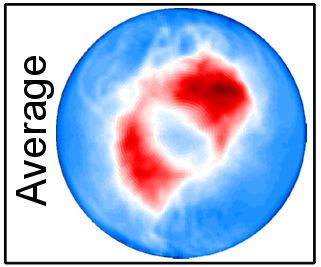
\includegraphics[width=1\textwidth]{graphs/dynamo/dyn_d100_mean_Br.png}\\
 \vfill
  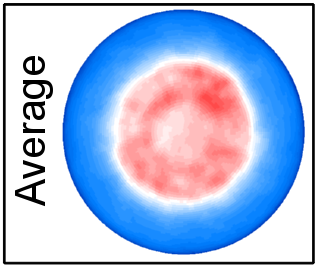
\includegraphics[width=\textwidth]{graphs/dynamo/dyn_d100_mean_q0_Br.png}
 \end{minipage}
 \caption{Time series of a north polar view on the radial magnetic field intensity at the CMB. \textbf{Top row:} Case \textbf{PFF100} (see table \ref{tab:data}). The field strength is highly time dependent but a preference for a structure with \textit{two} red patches of high intensity (azimuthal wave number $m=2$) is discernible. The imposed heat flux maxima lie at the top and the bottom, the minima on the right and left hand side in this view (see figure \ref{fig:fluxsketch}). \textbf{Bottom row:} Case \textbf{UFT100}. Like in case PFF100 above, the field behavior is highly time-dependent but in contrast to the heat flux pattern case, the system rather promotes structures with \textit{one} flux patch. The color scale ranges from -0.5 (dark blue) to 2.5 (dark red). The \textbf{right end} shows the long-term averaged data. }
 \label{fig:fluxpatches_snapshots}
 \end{figure} \noindent
The effect of a $\mathcal{Y}_2^2$ heat flux condition on thermo-chemical core convection was subject to the preceding section. In order to explore the influence of the new set of BCs in a geophysically more realistic context, i.e., planetary dynamos, a magnetic field will be included in this section. Although the term 'more realistic' is used here, the reader is reminded of the fact that the accessible parameter range, especially concerning the Ekman number, is far from being Earth-like. Furthermore, only some distinct properties of the geodynamo can be regarded in the scope of this study. \\
The generation of magnetic flux patches will be regarded in the context of a  \textit{thermo-chemical} dynamo model.\\ \par \noindent
A series of snapshots of the radial magnetic field component at the north pole, shown in figure \ref{fig:fluxpatches_snapshots}, top row, gives a first insight into the behavior of the magnetic field under the influence of the heat flux pattern: Patches of intense magnetic field wander, merge and detach again in a highly time-dependent manner. Yet, the number of \textit{two} patches seems to be preferred by the system and therefore the azimuthal wave number $m=2$ dominates the magnetic energy spectrum (not shown). This is attributed to the heterogeneous BC at the CMB that has the same azimuthal symmetry.\\
In contrast to that, figure \ref{fig:fluxpatches_snapshots}, bottom row, shows the uniform case with the same Rayleigh number. The magnetic field strength is comparable but the magnetic energy in the $m=2$ mode does not dominate the spectrum. Instead, the number of \textit{one} flux patch seems to be preferred. The corresponding long-term averaged fields at the right end of figure \ref{fig:fluxpatches_snapshots} confirm the impression received from the snapshots.  \\ \par \noindent
This part of the study is structured as follows: As an introduction, section \ref{sec:dyn_d020} explains the formation of the pattern induced magnetic flux patches, visible in figure \ref{fig:fluxpatches_snapshots}, with the help of a showcase. The subsequent chapter \ref{sec:delta_dependence} deals with the dual-forcing nature of the problem, before section \ref{sec:effect_pattern} relates the two preceding ones to each other and describes the effect of the heat flux pattern in the context of a changing driving mechanism. At last, chapter \ref{sec:robustness} checks the robustness of the results for other parameter regimes.\\In the following, all uniform cases will be denoted by \textbf{UFF} (uniform fixed flux), whereas \textbf{PFF} refers to the heat flux pattern cases. The former imply $q^*\!=\!0$, the latter $q^*\!=\!2$ (see section \ref{sec:flux_pattern}). All simulations conducted here are characterized by a high degree of time dependence so that the signature of the heat flux pattern is hard to identify in snapshots. Therefore, if not marked differently, only long-term averaged data from the statistically stationary state will be shown. Throughout this study, the magnetic Prandtl number will held constant at $\textrm{Pr}_\textrm{m}=3$. According to the previous chapter, the thermal and compositional Prandtl numbers are $\textrm{Pr}_\textrm{\tiny T}=0.3$ and $\textrm{Pr}_\textrm{\tiny C}=3$, respectively.
\begin{table}[H]
 \centering
 \begin{tabular}{l | c| c |c |c| c| c| c| c |c}
  \textbf{Case} &  $q^*$ & Ek	& $\textrm{Ra}_\textrm{\tiny T}\times \textrm{Ek}$& $\textrm{Ra}_\textrm{\tiny C} \times \textrm{Ek}$& $\gamma_\textrm{total}$& $\delta^*$& $\textrm{Re}_m$& $\Lambda$& $f_\textrm{dip}$ \\
  \hline
  \hline
\rule{0pt}{4ex}\textbf{PFF100} & 2&  $10^{-4}$ & $440$ &$0$ & $8.6$ & \textbf{100\%} & 284.8 & 26.5 & 62\% \\ 
  \textbf{PFF69}   &2&  $10^{-4}$ & $352$ & $88$ & 10 & \textbf{69\%}	& 254.9 & 23.3 & 64\% \\       
  \textbf{PFF36}    &2&  $10^{-4}$& 220 & 220 & 12 & \textbf{36\%} & 209.9 & 16.3 & 72\% \\
  \textbf{PFF12}   &\textbf{2}&  $\bm{10^{-4}}$ & \textbf{88} & \textbf{352} & \textbf{14} & \textbf{12\%} & \textbf{170.3} & \textbf{7.4} & \textbf{85\%} \\
  \textbf{PFF0}    &2&  $10^{-4}$& 0 & 440 & 15.4 &\textbf{0\%} & 139.5 & 4.8 & 92\% \\
  \hline
 \rule{0pt}{4ex}\textbf{UFF100} & 0&  $10^{-4}$ & $400$ & $0$ & 8.6 & \textbf{100\%}	& 300.5&	19.1&	59\% \\
  \textbf{UFF69} & 0 &  $10^{-4}$& 352 & 88 & 10 & \textbf{69\%} & 276.7&	15.3&	63\% \\
  \textbf{UFF36}    &0&  $10^{-4}$& 220 & 220 & 12 & \textbf{36\%} & 210.2&	12.4&	72\% \\
  \textbf{UFF12} & 0 &  $10^{-4}$ & 88 & 352 & 14 & \textbf{12\%} & 151.8&	6.9&	88\% \\
  \textbf{UFF0}	& 0 & $10^{-4}$& 0 & 440 & 15.4 &\textbf{0\%} & 139.5&	4.8&	92\% 
 \end{tabular}
\caption{Overview of the parameters and the cases regarded in this section with the associated diagnostic quantities: Magnetic Reynolds number Re$_m$, Elsasser number $\Lambda$ and relative strength of the magnetic dipole component $f_\textrm{dip}$, all defined in section \ref{sec:diagnostics}. The case PFF12, highlighted in bold, serves as showcase in section \ref{sec:dyn_d020}. \textbf{PFF} stands for a fixed flux condition including the heat flux pattern, \textbf{UFF} for the uniform fixed flux BC.}
\label{tab:data}
\end{table}
\subsection{The patch generation mechanism: A showcase}
\label{sec:dyn_d020}
\begin{figure}[t]
\centering
      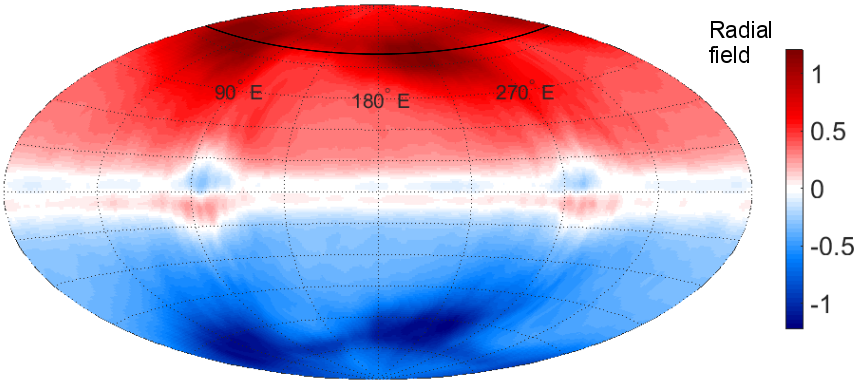
\includegraphics[width = 0.7\textwidth]{graphs/dynamo/flux_patches_d20_2.png}
  \caption{Hammer-Aitov surface projection of the radial magnetic field near the CMB at $r=1.485$. Two patches of high intensity magnetic field are located at $\sim$45$^\circ$ and $225^\circ$ in the northern and the southern hemisphere. The black line at a polar angle of $25^\circ$ is subject to the graph in figure \ref{fig:divLat_Br}.}
  \label{fig:surface_Br_d20}
\end{figure} \noindent
This section is dedicated to the formation mechanism of patches of intense magnetic field at the CMB (visible in figure \ref{fig:fluxpatches_snapshots}). It will be seen that analogies to the preceding chapter \ref{sec:thermo-chemical} exist, where the compositional field heterogeneities shown in figure \ref{fig:vort_chem} got a similar origin as the magnetic flux patches in the dynamo case.\\ \par \noindent
Case PFF12 (see table \ref{tab:data}) with of portion of $\delta^* = 12$ \% thermal forcing was chosen as a showcase. Although the uniform chemical forcing dominates in this case, the influence of the heat flux pattern is clearly visible in the surface projection of the radial magnetic field in figure \ref{fig:surface_Br_d20}. Patches of intense magnetic flux lie at  $\sim$45$^\circ$ and $225^\circ$E in the northern and the southern hemisphere. They are each shifted $45^\circ$ west of the longitudes of maximum heat flux ($90^\circ$ and $270^\circ$, see figure \ref{fig:fluxsketch}). \\ \par \noindent
In section \ref{sec:attached_columns}, the flow convergence and divergence at the top of anticyclones and cyclones, respectively, controls the surface distribution of the chemical component (see figure \ref{fig:vort_chem}). In a comparable way, magnetic field can be locally collected (intensified) and expelled (weakened) by cyclonic and anticyclonic motion at the CMB in an advection process. A necessary condition for this to happen can be understood in the framework of \textit{Alfv\'{e}n's theorem} that states:\\ \par
\textit{Magnetic flux tubes move with fluid particles as if they were frozen into it \textbf{if} the fluid has infinite conductivity} \citep{davidson2001introduction, roberts2007theory}.\\ \par \noindent
Infinite conductivity goes along with zero magnetic diffusion. Therefore, the relative importance of magnetic diffusion in a system (see the the second term on the rhs of equation \eqref{eq:induction^}) decides whether magnetic field collection and expulsion by advection can serve as an explanation for the flux patches. The \textit{magnetic Reynolds number} estimates the ratio of magnetic advection to diffusion \citep{rieutord2014fluid} and therefore is the relevant quantity in this context \citep{christensen2011geodynamo}. Table \ref{tab:data} shows that the magnetic Reynolds number for this (Re$_m$ = 170.3) and for the other cases is of order $\mathcal{O}$(100). It becomes obvious that advection dominates diffusion by far and therefore the above process is likely play a role in the generation of the flux patches. \\ \par \noindent
\begin{figure}[t]
\centering
   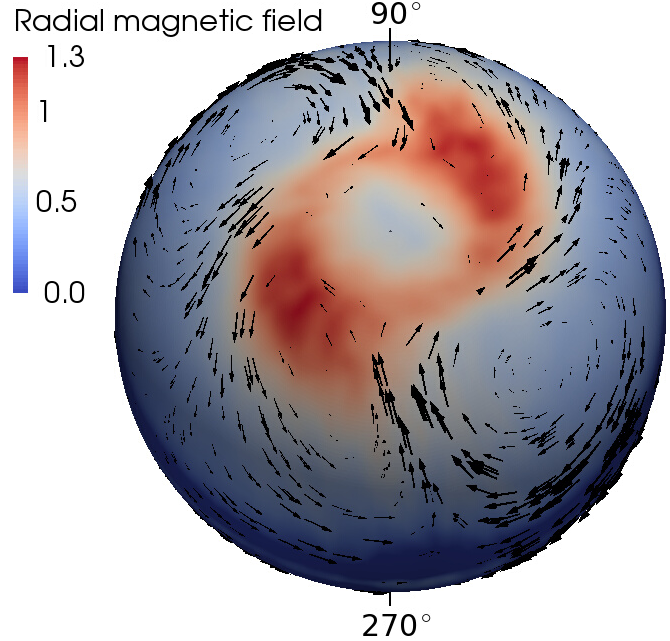
\includegraphics[width = 0.5\textwidth]{graphs/dynamo/dyn_d20_vectorfield_Br.png}
 \caption{Surface flow field (scaled by the flow magnitude) and radial magnetic field component near the CMB at $r = 1.485$ for case PFF12. In the facing hemisphere, a dominant anticyclone with the center at $\sim 315^\circ$E and a weaker, bended cyclone with the center at $\sim 230^\circ$E are visible. Intense magnetic field correlates with the cyclonic region. View from a polar angle of $20^\circ$, the north pole is located in the middle of the central blue region.  }
 \label{fig:dyn_d20_vectorfield_Br}
\end{figure}\noindent
Figure \ref{fig:dyn_d20_vectorfield_Br} shows a north polar view of the three dimensional surface of the spherical shell at a radial level $r=1.485$, tilted by the polar angle $\vartheta = 20^\circ$. A schematic overview of the important features of the velocity and the magnetic field in this view can be found in figure \ref{fig:sketch_patches}, where red (blue) patches represent cyclones (anticyclones) and black crosses stand for patches of increased radial magnetic field strength (flux patches).  \\
The surface flow field (black arrows in figure \ref{fig:dyn_d20_vectorfield_Br}) exhibits a pattern of two regions of anticyclonic motion around $135^\circ$ and $315^\circ$E (blue patches in figure \ref{fig:sketch_patches}) and two regions of cyclonic motion in between at $45^\circ$ and $235^\circ$ (red patches). Two fields of increased radial magnetic field strength (black crosses) form adjacent to the intersection of the TC and the CMB. The flux patch generation process can be understood regarding the azimuthal profile of the radial field $B_r$ and the horizontal divergence of the velocity field $[\bm \nabla \cdot \bm u]_\textrm{\tiny H}$, shown in figure \ref{fig:divLat_Br}: \\
The radial magnetic field is locally intensified due to the convergent flow caused by the cyclonic motion at the CMB. At the same time, the divergent flow on top of the anticyclones expels field lines and therefore causes the field strength to decrease in that regions. Thus, both mechanisms, field collection and expulsion, take part in determining the magnetic field geometry. \\
\begin{figure}[t]
\begin{minipage}{0.46\textwidth}
  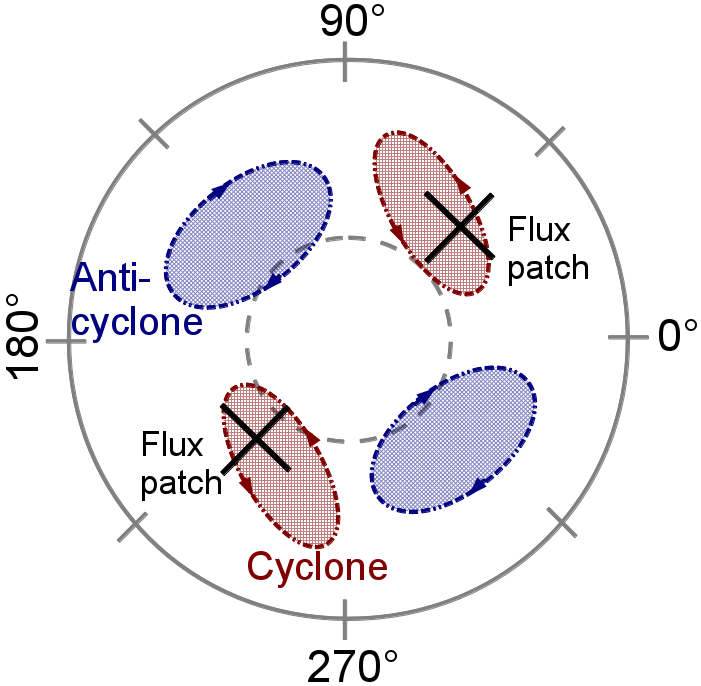
\includegraphics[width=\textwidth]{sketches/Patches_cyclones.png}
  \caption{Sketch of a north polar view on the vorticity distribution and the location of the magnetic flux patches for case PFF12, shown in figure \ref{fig:dyn_d20_vectorfield_Br}. Red patches mark cyclones, blue patches anticyclones and the black crosses indicate the position of the flux patches. The gray dashed line represents the intersection of the TC with the CMB. }
  \label{fig:sketch_patches}
\end{minipage}
\hfill
 \begin{minipage}{0.51\textwidth}
 \vspace{2mm}
 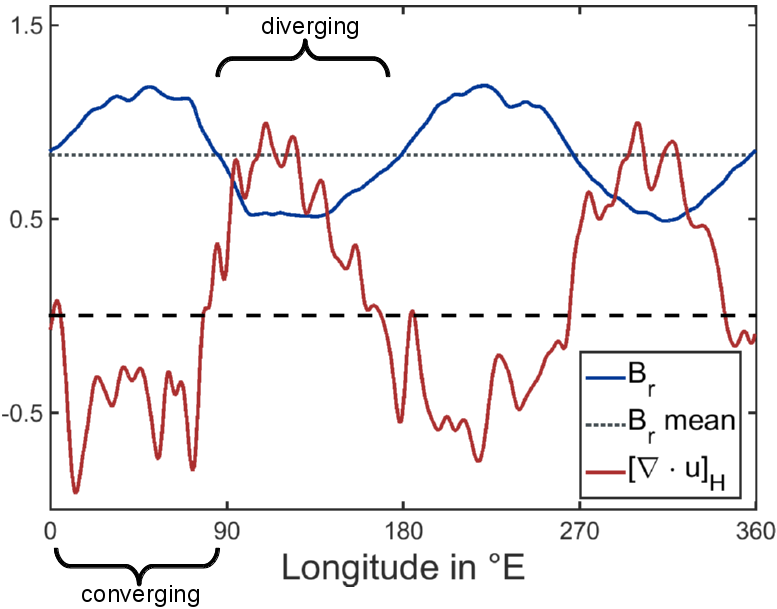
\includegraphics[width = \textwidth]{graphs/dynamo/d20_divLat_Br3.png}
 \vspace*{1mm}
  \caption{Azimuthal profile of the radial magnetic field $B_r$ (blue) and the horizontal divergence of the velocity field $[\bm \nabla \cdot \bm u]_\textrm{\tiny H}$ (red), normalized by its maximum. A negative (positive) divergence characterizes a convergent (divergent) flow, visible around $45^\circ$ and $235^\circ$E ($120^\circ$ and $300^\circ$E), where $B_r$ is maximum (minimum). Profile taken at $r=1.485$ and $\theta = 25^\circ$, shown by the black line in figure \ref{fig:surface_Br_d20}. }
  \label{fig:divLat_Br}
 \end{minipage}
\end{figure}\noindent
\subsection{Changing the driving mechanism}
\label{sec:delta_dependence}
The key quality of a \textit{thermo-chemical} model of core convection is the possibility to explore the interplay of two different driving mechanisms with distinct Prandtl numbers in one system. How the system dynamics depend on the choice of the ratio between thermal and compositional driving is the central question. It was recently studied for the non-magnetic case by \citet{breuer2010thermochemically} and \citet{trumper2012numerical} or the dynamo case by \citet{manglik2010dynamo} and \citet{takahashi2014double}. The choice of a distinct forcing ratio in case of the models cited above means to strengthen either the thermal component that is equipped with a Prandtl number $\textrm{Pr}_\textrm{\tiny T}<1$ or the compositional component that commonly goes along with $\textrm{Pr}_\textrm{\tiny C}\geq1$. If $\textrm{Pr}$ is less than unity, inertial processes gain importance, whereas $\textrm{Pr}$ greater one emphasizes diffusion of heat and composition, respectively.\\ \par \noindent
In contrast to that, changing the forcing ratio $\delta^*$, as it is done here (see section \ref{sec:thermal/chemical}), has \textit{three} major implications:
\begin{enumerate}[(A)]
 \item The BC for the thermal component is of the \textit{Neumann} type (fixed heat flux), whereas the compositional field underlies \textit{Dirichlet} conditions (fixed composition).
 \item The thermal \textit{Prandtl number} is chosen to be $\textrm{Pr}_\textrm{\tiny T}=0.3$ and the chemical $\textrm{Pr}_\textrm{\tiny C}=3$.
 \item Only the temperature field underlies the CMB \textit{heat flux pattern}, whereas the compositional BC is \textit{uniform}.
\end{enumerate}
Each of the points mentioned is expected to have an effect on the behavior of the system. The task is now to identify the individual effects of (A), (B) and (C) in the data and to separate them from each other as good as possible. \\ \par
\begin{figure}[t]
\begin{minipage}{0.308\textwidth}
  \centering
   \caption*{(a) Elsasser $\Lambda$}
 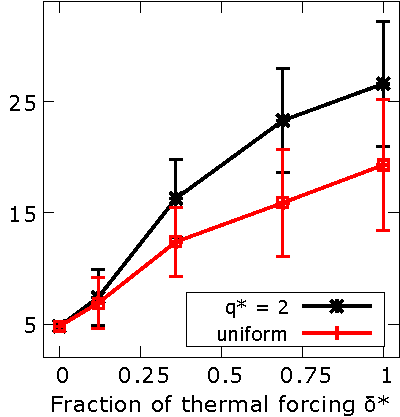
\includegraphics[width = 0.99\textwidth]{results/els-crop.pdf}
\end{minipage}
\hfill
\begin{minipage}{0.32\textwidth}
  \centering
   \caption*{(b) Magnetic Reynolds Re$_m$}
 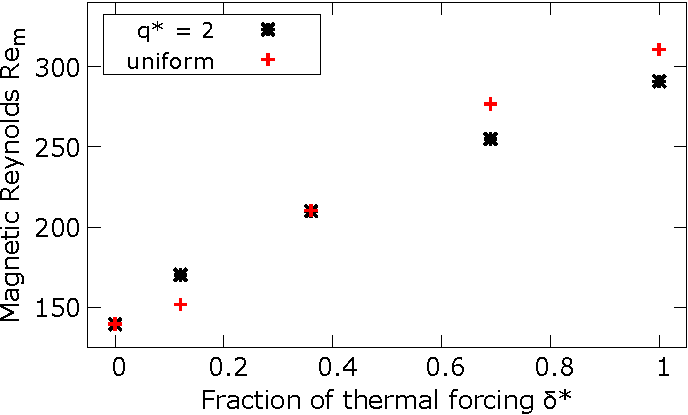
\includegraphics[width = 0.99\textwidth]{results/reym-crop.pdf}
\end{minipage}
\hfill
\begin{minipage}{0.32\textwidth}
  \centering
   \caption*{(c) Toroidal kin. energy $f_\textrm{tor}$}
 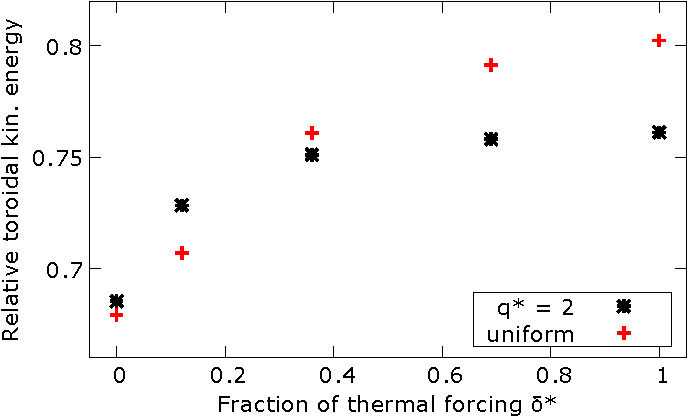
\includegraphics[width = 0.99 \textwidth]{results/relTor-crop.pdf}
\end{minipage}
 \caption{(a) Elsasser number, (b) magnetic Reynolds number Re$_m$ and (c) portion of toroidal kinetic energy $f_\textrm{tor}$ (ratio of the toroidal kinetic energy to the total kinetic energy) for different forcing ratios $\delta^*$ for the uniform case UFF as well as for the case PFF with $q^*=2$. The data originates from the statistically stationary state. The errorbars in (a) indicate the standard deviation.}
   \label{fig:els_reym}
\end{figure} \noindent
Figure \ref{fig:els_reym} summarizes some of the results of the Parameter study on the dependence on $\delta^*$ (also shown in table \ref{tab:data}). The heat flux pattern case PFF (black lines) is presented as well as the case UFF (red lines), that includes uniform heat flux BCs in the thermal component (see also table \ref{tab:data}). The following sections are each dedicated to one specific observation induced by the transition from $\delta^*\!=\!0\%$ to $\delta^*\!=\!100\%$.
\subsubsection{Magnetic field strength}
\label{sec:magnetic_field_strength}
\citet{sakuraba2009generation} report the generation of a strong magnetic field in their dynamo model with a uniform heat flux imposed at the outer spherical boundary. The observation is remarkable because they used a comparatively low Ekman number ($\textrm{Ek} = 5 \times 10^{-7}$). In this regime, the possibility of an efficient field production was questioned due to the extreme refinement of the azimuthal length scales when increasing the rotation rate \citep{sakuraba2009generation}. In contrast to the widely used fixed temperature condition, a fixed flux condition allows lateral temperature gradients to develop at the CMB. \citet{gibbons2007convection} and \citet{sakuraba2009generation} therefore expect large scale zonal flows to develop in a thermal wind mechanism (Roberts, 2007; see also section \ref{sec:thermal_wind}). As such flows are assumed to be a necessary ingredient for an efficient dynamo process, the fixed flux condition indirectly has a positive effect on the magnetic field strength \citep{hori2012influence}.\\ 
The dependence of the magnetic field morphology and efficiency of the dynamo process on the Prandtl number was studied by \citet{simitev2005prandtl} and \citet{busse2006parameter}. The amount of DR generated by Reynolds stresses (see \citet{busse2002convective, christensen2011geodynamo}) is inversely related to the Prandtl number \citep{simitev2005prandtl}: In the low Prandtl number thermal regime, the DR is much stronger than in the compositional regime with $\textrm{Pr}_\textrm{\tiny C} >1$. As a consequence, the toroidal magnetic field produced by DR in an $\omega$-effect is stronger in a thermally than in a compositionally driven case. The result is an intensification of the dynamo process and therefore the magnetic field.  \\ \par \noindent
The Elsasser number $\Lambda$ compares the influence of the Lorentz force to that of the Coriolis force in the equation of momentum \citep{davidson2001introduction}. As the rotation rate is held constant here, $\Lambda$ serves as a measure for the strength of the magnetic field. Figure \ref{fig:els_reym}(a) shows $\Lambda$ for the different forcing ratios $\delta^*$ (see table \ref{tab:data}) for the uniform case UFF and for the heat flux pattern case PFF with $q^*\!=\!2$.  In both scenarios, the field strength increases roughly linearly with $\delta^*$. According to the preceding discussion, this effect can be attributed to either the transition from a fixed composition BC at $\delta^* = 0\%$ to a fixed heat flux BC at $\delta^* = 100\%$ or to a transition from the low to the high Prandtl number regime. A combination of both reasons is likely to be an explanation. A more detailed discussion is beyond the scope of this study. \\ \par \noindent
Figure \ref{fig:els_reym}(a) allows two more observations: (a) The standard deviation of the temporal averages of $\Lambda$ increases with increasing $\delta^*$ for case PFF and UFF. (b) The magnetic energy is higher for the heterogeneous case PFF (black line) than for the uniform case UFF (red line). \\
The standard deviation measures the strength of the temporal variation of the magnetic field. As this observation cannot be attributed to the heat flux pattern, it has its origin either in the the varying Prandtl number or in the transition from Dirichlet to Neumann BCs. A further investigation of this question would be interesting. E.g. a comparison with the temporal variation of the geomagnetic field data could offer information about the driving mechanism in the Earth's core. \\
Observation (b) is likely to be a consequence of the enlargement of the \textit{mean} azimuthal flow scale due to the enhancement of the (low) azimuthal mode $m\!=\!2$, induced by the $\mathcal{Y}^2_2$ heat flux pattern (the mode enhancement through the pattern was also reported by \citet{hori2014ancient} and \citet{dietrich2016core}). As previously discussed, flow scale refinement impedes the magnetic field production, whereas the heterogeneous temperature BC promotes large scales on which the dynamo process works more efficient.
\subsubsection{Kinetic energy}
\label{sec:kinetic_energy}
The magnetic Reynolds number estimates the relation between the advection and the diffusion of the magnetic field. As it contains the rms-velocity, it indirectly measures the kinetic energy. Like the Elsasser number, $\textrm{Re}_m$ increases roughly linearly with $\delta^*$ (see figure \ref{fig:els_reym}(b)) for PFF and UFF.  \\
The zonal flow originating in a thermal wind, mentioned at the beginning of the preceding section, is a possible explanation for the increase in Re$_m$. The growing amount of DR production due to a transition to $\textrm{Pr}_\textrm{\tiny T}=0.3$, could likewise be a reason, also observed in \citet{breuer2010thermochemically} for the non-magnetic case. \\
Figure \ref{fig:els_reym}(c) that shows the ratio of the toroidal kinetic energy to the total kinetic energy $f_\textrm{tor}$ assists both ideas: For UFF, the increase of the kinetic energy involves an increase of its relative toroidal part, a proxy for the azimuthal component of the velocity field. Whether this increase originates in a thermal wind like zonal flow (connected to (A)) or in the DR (connected to (B)) is difficult to decide here. \\
For the heat flux pattern case PFF, figures \ref{fig:els_reym}(a) and (c) suggest the assumption that a thermal wind mechanism plays the major role in the behavior of Re$_m$. Lateral temperature gradients at the CMB, induced by the flux pattern, cause a significant increase of the toroidal kinetic energy if they enter the system to a minor degree ($\delta^* = 12\%$). With increasing $\delta^*$, this lateral heterogeneity impedes large scale zonal flows to develop at the cost of the toroidal kinetic energy (see the kink in the black curve in figure \ref{fig:els_reym}(c)). This again reduces Re$_m$ compared to the uniform case for $\delta^*\!=\!69\%$ and $\delta^*\!=\!100\%$.

\subsubsection{Dipolarity of the magnetic field}
\label{sec:reldip}
The relative strength of the magnetic dipole component at the CMB is a measure that is accessible for dynamo simulations as well as for the geomagnetic field. Therefore it may serve as an indicator for the degree to which a dynamo model can be called Earth-like. The definition of the dipole strength $f_\textrm{dip}$ is given in section \ref{sec:diagnostics}. \\ \par \noindent
Figure \ref{fig:reldip} shows a decrease of $f_\textrm{dip}$ for the transition from purely chemical ($\delta^*=0\%$) to purely thermal convection ($\delta^*=100\%$) for the heat flux pattern case PFF (black line) as well es for the uniform case UFF (red line). \citet{sreenivasan2006role} and \citet{christensen2006scaling} argue that the Rossby number $Ro$, measuring the importance of inertia compared to that of rotation in the force balance, plays a crucial role for the dipolarity of the magnetic field. This suggests that the transition from Pr$_\textrm{\tiny C} = 3$ to Pr$_\textrm{\tiny T}=0.3$ (B) is responsible for the drop in $f_\textrm{dip}$ because the Prandtl number weights the inertia term in the equation of momentum. \citet{busse2006parameter} likewise report a reciprocal dependence between dipolarity and Prandtl number. An explanation with the heat flux pattern (C) can be neglected, as PFF and UFF do not differ significantly in their behavior and (A) as well is expected to play only a minor role for the dipolarity. \\ \par \noindent
The black dotted line in figure \ref{fig:reldip} represents the relative dipole strength of the present geomagnetic field, $f_\textrm{dip}=0.65$ \citep{finlay2010international}. \citet{takahashi2014double} studies thermo-chemical dynamo action with regard to the dipolarity and defines this value of $f_\textrm{dip}$ as a threshold for the \textit{dipolar regime} (the Earth's present magnetic field is supposed to be in a state of a relatively low dipole strength). He expects dynamos to be part of this regime as long as their high Prandtl number chemical forcing accounts for at least $40\%$ of the total forcing. \\ 
 The definition of the forcing ratio and the choice of the Prandtl numbers Pr$_\textrm{\tiny T}$ and Pr$_\textrm{\tiny C}$ in this work slightly differ from his model, nevertheless, figure \ref{fig:reldip} reveals a similar behavior. The purely thermally driven case PFF100 is characterized by a value of $f_\textrm{dip}$ that seems unrealistic for the present state of the Earth. Only PFF0, PFF12 and PFF36 clearly exceed the threshold for the dipolar regime. \\
 The observations made in this section are in line with the findings of \citet{takahashi2014double} and suggest that a certain portion of chemical forcing is mandatory in order to reach Earth-like values for the relative dipole strength. Furthermore, it is important to notice that the magnetic dipole remains unaffected by the heterogeneity of the thermal BC. 
\begin{figure}[t]
 \centering
    \caption*{Relative dipole $f_\textrm{dip}$}
    \centering
   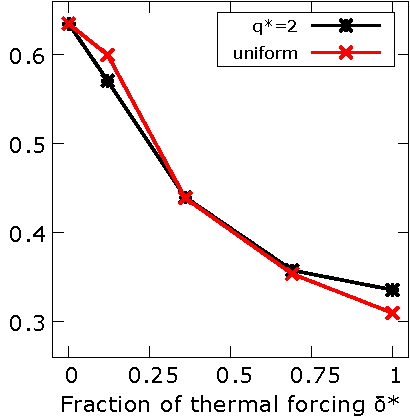
\includegraphics[width = 0.5\textwidth]{results/reldip-crop.pdf}
   \vspace{5mm}
 \caption{Relative dipole strength $f_\textrm{dip}$ (see section \ref{sec:diagnostics} for a definition) for different $\delta^*$ for the heat flux pattern case PFF (black line) and the uniform case UFF (red line). The black dotted line shows the value for today's geomagnetic field $f_\textrm{dip} = 0.65$ \citep{finlay2010international}.}
 \label{fig:reldip}
\end{figure} \noindent

\subsection{The heat flux pattern in the context of a changing driving mechanism}
\label{sec:effect_pattern}
The goal of this section is to integrate the findings of section \ref{sec:dyn_d020} concerning the magnetic flux patch generation into the context of the changing driving mechanism discussed in section \ref{sec:delta_dependence}. It was already shown that the effect of the heat flux pattern persists even if the relative influence of the thermal driving component makes up only 12\% (see also figure \ref{fig:relamp} at the end of this section). A justification for the choice of PFF12 as a showcase in the above section will be given and the relation between the corresponding effect and the changing of the forcing ratio clarified. \\ \par \noindent
The intensification of the magnetic field, measured in terms of the Elsasser number, originating in the increase of the thermal forcing ratio can be related to the behavior of the dynamo under the influence of the heat flux pattern. Regarding the ratios of magnetic to kinetic energy (they are at least of order $\mathcal{O}$(10) for all cases) and the Elsasser numbers (see table \ref{tab:data}) which measure the relative importance of the Lorentz force compared to the Coriolis force, it is reasonable to assume that the system belongs to the \textit{strong field regime} \citep{zhang2000magnetohydrodynamics}. This means that the Lorentz force has a significant effect on the flow field. \\
\citet{sakuraba2000effect} apply a uniform magnetic field $\bm B_0$ parallel to the rotation axis to their magnetoconvection model in order to explore the influence of the strength of $\bm B_0$ on the convection dynamics. For the strong field regime, they find an enhancement of anticyclonic vortices in the equatorial plane that is explained with the need to store the large amounts of magnetic field present in the system. Anticyclones create a convergent flow in the equatorial plane (see the sketch in figure \ref{fig:secondary_circulation}) that gathers magnetic flux and thus serve as a storage for magnetic energy. The Lorentz force in an anticyclone is oriented outward and therefore works together with the pressure gradient force against the inward directed Coriolis force. As a result, the anticyclone grows in order to balance the additional impact of the Lorentz force \citep{sakuraba2000effect}. \\
A similar observation was made by \citet{ishihara2002dynamo} who performed a self-sustained dynamo simulation. They describe a cyclic process in which an anticyclone grows, increasingly collects and intensifies magnetic flux by field line stretching and then breaks down due to the rising power of the outward directed Lorentz force before it grows again. \\ \par \noindent
\begin{figure}[t]
\begin{subfigure}[b]{0.49\textwidth}
 \caption*{\textbf{Case PFF12}}
 \begin{minipage}{0.46 \textwidth}
 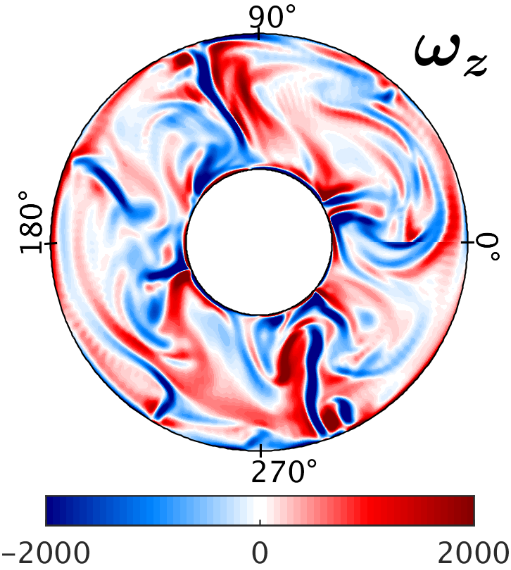
\includegraphics[width = \textwidth]{graphs/dynamo/driving_mechs/d020_vorticity.png}\\
 \vfill
  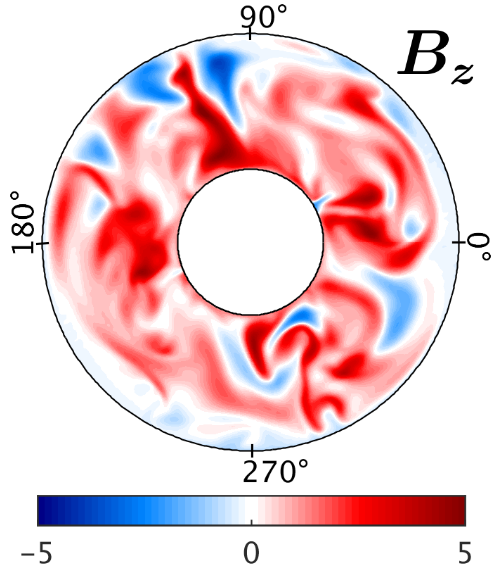
\includegraphics[width = \textwidth]{graphs/dynamo/driving_mechs/d020_Br.png}
 \end{minipage}
\hfill
 \begin{minipage}{0.46 \textwidth}
 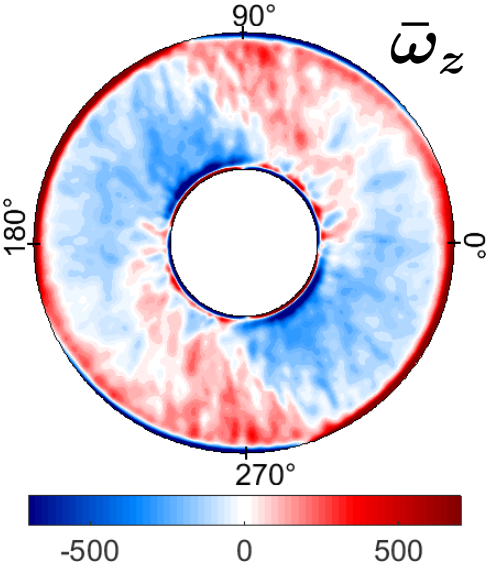
\includegraphics[width = \textwidth]{graphs/dynamo/driving_mechs/vorticity_eq_d20-trim.png}\\
 \vfill
  \includegraphics[width = \textwidth]{graphs/dynamo/driving_mechs/dyn_q2_440_d020_mean_Br-trim.png} 
 \end{minipage}
 \hfill
 \end{subfigure}
 \begin{subfigure}[b]{0.49\textwidth}
  \caption*{\textbf{Case PFF100}}
 \vrule width 3pt
 \hfill
  \begin{minipage}{0.46 \textwidth}
 \includegraphics[width = 1.\textwidth]{graphs/dynamo/driving_mechs/d100_vorticity.png}\\
 \vfill
  \includegraphics[width = 1.\textwidth]{graphs/dynamo/driving_mechs/d100_Br.png} 
 \end{minipage}
 \hfill
  \begin{minipage}{0.46 \textwidth}
 \includegraphics[width = \textwidth]{graphs/dynamo/driving_mechs/vorticity_eq_d100-trim.png}\\
 \vfill
  \includegraphics[width = \textwidth]{graphs/dynamo/driving_mechs/Br_d100-trim.png} 
 \end{minipage}
  \end{subfigure}
  \caption{Equatorial views on the $z$-component of vorticity (top row) and the the axial magnetic magnetic field for case PFF12 ($\delta^* = 12$\%, left panel) and PFF100 ($\delta^*=100$\%, right panel). The first column in each panel shows snapshots ($ \bm{\omega_z}$ and $\bm{B_z}$), the second column long-term averages ($\bm{\bar \omega_z}$ and $\bm{\bar {B}_z$}). }
  \label{fig:anticyclones_dominance}
\end{figure} \noindent
Figure \ref{fig:anticyclones_dominance} shows equatorial views of the axial vorticity (top row) and the axial component (parallel to the $z$-axis) of the magnetic field (bottom row). Case PFF12 is subject to the left panel, whereas the right panel depicts case PFF100. The left column in each panel shows snapshots ($ \bm{\omega_z}$ and $\bm{B_z}$), the right panel long-term averaged quantities ($\bm{\bar \omega_z}$ and $\bm{\bar {B}_z$}). \\
When comparing the red and the blue regions in the snapshots of the vorticity in case PFF100, a dominance of anticyclonic (blue) structures ($\bm{\omega_z} < 0$) over cyclonic (red) structures is discernible. Two large regions with $\bm{\omega_z}<0$ lie at $90^\circ$ and $270^\circ$E close to the ICB. They are each accompanied by patches of high intensity magnetic flux, visible in the subfigure beneath. \\
In contrast to that, the vorticity pattern for PFF12 reveals smaller scales and the regions of negative and positive vorticity are present to the same extent. Nevertheless, a correlation between $\bm{\omega_z}$ and $\bm{B_z}$ exists, which is in line with what was described in the beginning of this section. The fact that the length scales in the predominantly compositionally driven case are smaller, agrees with the work of \citet{trumper2012numerical} and can be explained with the relatively low compositional diffusivity (high Prandtl number $\textrm{Pr}_\textrm{\tiny C}$) that makes the smoothing of small scale structures less efficient than in the thermally driven case. \\
The long-term averaged fields (right column in each panel in figure \ref{fig:anticyclones_dominance}) support the impression received from the snapshots. In case PFF12, positive and negative vorticity are nearly equally distributed but clearly show the influence of the $\mathcal{Y}_2^2$ heat flux pattern. In the purely thermally driven case PFF100, the impact of the heterogeneous BC is only visible close to the CMB, where two bands of positive vorticity got their maximum $\sim 30^\circ$ west of the longitude of maximum CMB heat flux. The averaged axial magnetic fields ($\bm{\bar {B}_z}$) reflect what could already be seen in the vorticity distribution. In case PFF12, anticyclones intensify magnetic flux, whereas cyclones expel and therefore weaken the field. PFF100 provides, in line with the vorticity field, a nearly uniform distribution of  $\bm{\bar{B}_z}$. \\ \par \noindent
\begin{figure}[t]
 \begin{minipage}{0.50\textwidth}
  \includegraphics[width = 0.97\textwidth]{graphs/dynamo/dyn_d100_vectorfield_Br.png}
  \caption{Surface flow field (scaled by the flow magnitude) and radial magnetic field component near the CMB at $r = 1.485$ for case PFF100. In the facing hemisphere, a dominant anticyclone with the center at $\sim 315^\circ$E is visible. The cyclonic region around 230$^\circ$ is less pronounced than in case PFF12, shown in figure \ref{fig:dyn_d20_vectorfield_Br}. Magnetic flux patches are located in between the anticyclones. View from a polar angle of $20^\circ$, the north pole is located in the middle of the central blue region.}
  \label{fig:d100_vectorfield_Br}
 \end{minipage}
\hfill
\begin{minipage}{0.46\textwidth}
 \vspace{8mm}
\includegraphics[width = 0.97\textwidth]{graphs/dynamo/d100_divLat_Br_mean.png}
 \vspace{7mm}
\caption{Azimuthal profile of the radial magnetic field $B_r$ (blue) and the horizontal divergence of the velocity field $[\bm \nabla \cdot \bm u]_\textrm{\tiny H}$ (red), normalized by its maximum. Divergent flow (related to positive lateral divergence, $120^\circ$ and $300^\circ$E)) dominates in this case and correlates with the minima of $B_r$ (same graph as in figure \ref{fig:divLat_Br}, but for case PFF100).}
% \caption{Same as figure \ref{fig:divLat_Br} but for case PFF100. Here, instead of plotting $B_r$ and $[\bm \nabla \cdot \bm u]_\textrm{\tiny H}$ for one fixed latitude, the data is averaged over the surface region that contains the magnetic flux patch, i.e. from $\vartheta = 17^\circ$ to $\vartheta = 35^\circ$.}
\label{fig:d100_divLat_Br_mean}
\end{minipage}
\end{figure}
The previously described observations from figure \ref{fig:anticyclones_dominance} are assumed to stem from the magnetic field strength, measured by the Elsasser number $\Lambda$. As it increases with increasing $\delta^*$ (see figure \ref{fig:els_reym}(a)), it promotes anticyclonic vortices in the equatorial plane and thereby suppresses cyclonic ones. This process agrees well with what \citet{sakuraba2000effect} and \citet{ishihara2002dynamo} report for their models. The dominance of negative vorticity close to the ICB in the equatorial plane has implications for the whole flow field and thereby for the magnetic field near the CMB. \\ \par \noindent
Figures \ref{fig:d100_vectorfield_Br} and \ref{fig:d100_divLat_Br_mean} refer to case PFF100 and correspond to figures \ref{fig:dyn_d20_vectorfield_Br} and \ref{fig:divLat_Br}  from section \ref{sec:dyn_d020}, where the flux patch generation mechanism was discussed exemplary for case PFF12. The dominance of the negative vorticity in the equatorial plane in case PFF100 matches the significant enlargement of the anticyclonic vortex visible in the surface flow field around $315^\circ$ (compare figure \ref{fig:d100_vectorfield_Br} and \ref{fig:dyn_d20_vectorfield_Br}). In return, the surface cyclone with its center at 230$^\circ$ shrinks and becomes weaker. This implies an uneven distribution of the horizontal divergence of the velocity field $[\bm \nabla \cdot \bm u]_\textrm{\tiny H}$, shown in figure \ref{fig:d100_divLat_Br_mean} (red line). The horizontal divergence (connected to anticyclones at the CMB) is significantly stronger than the convergence (negative divergence, connected to cyclones at the CMB). The magnetic field geometry at the CMB in case PFF100 is thus rather induced by the \textit{expulsion} of magnetic flux than by the \textit{collection} of magnetic field lines. The divergent flow on top of the anticyclones pushes the field towards the regions in between, where stronger cyclones were located in case PFF12. Hence, flux patches are located on top of the cyclones like before, although these play only a minor role in their formation.\\ \par \noindent
Figure \ref{fig:relamp} shows the relative flux patch amplitude $\mathcal{P}$ for the different values of $\delta^*$. It is defined as the ratio of the amplitude of the radial magnetic flux patches to the mean value of the radial magnetic field in the corresponding latitude.  \\
$\mathcal{P}$, a measure for the strength of the effect of the $\mathcal{Y}_2^2$ heat flux pattern, does not significantly decrease as the thermal forcing loses importance for decreasing values of $\delta^*$. In section \ref{sec:dyn_d020} and \ref{sec:effect_pattern} the flux patch generation mechanisms for case PFF12 and PFF100 were discussed in detail. Obviously, the two are nearly equally efficient and do not depend on the relative importance of the thermal forcing. The fact that the uniform chemical forcing does not impede the flux patch formation supports the view that the characteristic features of thermally and compositionally driven convection rather \textit{superpose} each other than really \textit{interact} \citep{trumper2012numerical}.
\begin{figure}[b!]
 \centering
    \caption*{Relative patch amplitude $\mathcal{P}$}
   \includegraphics[width = 0.5\textwidth]{results/relamp-crop.pdf}
    \vspace{1mm}
    \caption{Relative amplitude of the magnetic flux patches $\mathcal{P}$ for the different forcing ratios $\delta^*$ for case PFF. The data is taken from the statistically stationary state. }
 \label{fig:relamp}
 \end{figure} \noindent
A comparison of the magnetic field that emerges under the influence of the $\mathcal{Y}_2^2$ BC  (e.g. figure \ref{fig:surface_Br_d20} for $\delta^* = 12\%$) and the present geomagnetic field (see figure \ref{fig:pomm}) reveals that the heterogeneous BC is able to reproduce the two magnetic flux lobes in each hemisphere at high latitudes properly. Other features of figure \ref{fig:pomm}, i.e., a more complex structure and reverse flux patches, remain unaddressed in the scope of this study. The use of a more realistic and hence more complex heat flux pattern is one possibility to improve the agreement with geomagnetic data \citep{olson2015core}. \\  
The model at hand allows to study the joint action of a thermally forcing component under the influence of a heterogeneous CMB heat flux condition and a uniform compositionally forcing agent which is only indirectly affected by the pattern (see figure \ref{fig:vort_chem}) for various $\delta^*$. According to figure \ref{fig:relamp} and the previous discussion, the effect of the heat flux pattern persists over a wide range of the $\delta^*$-space. It is hence possible to observe characteristic features of the geomagnetic field (e.g. long lasting, stationary magnetic flux patches \citep{gubbins1987morphology}) in scenarios which are predominantly compositionally forced (as it is supposed to be for the Earth \citep{braginsky1995equations}) and therefore exhibit typical properties of that forcing agent, too. One of the properties typical of the compositionally dominated cases is a strong magnetic dipole, discussed in section \ref{sec:reldip}, additional can be found in \citet{trumper2012numerical} and \citet{trumper2014thermo}. Compared to the single forcing (codensity) models that were recently used to study heterogeneous CMB heat flux \citep{olson2002time,aubert2008thermochemical,hori2014ancient}, this model, combining thermal and compositional forcing, is able to produce a wider range of different behavior observable in the Earth's and other planetary dynamos.
\subsection{Robustness of the results}
\label{sec:robustness}
All results presented so far in section \ref{sec:dynamo} refer to the cases PFF and UFF that were all conducted with a total Rayleigh number $\textrm{Ra}_\textrm{total}\!=\!440\times 10^4$ and an Ekman number $\textrm{Ek}\!=\!10^{-4}$ (see table \ref{tab:data}). In order to draw any conclusions relevant for the field of planetary cores, the robustness of the observations has to be checked, i.e. the study has to be extended to other parameters. Although it is impossible to reach a \textit{realistic} parameter regime, as in most problems linked to dynamos, a step in the right direction can be made. In the following, the heat flux pattern amplitude will be held fixed at $q^*=2$. 
\begin{figure}[t]
 \begin{minipage}[t]{0.47\textwidth}
 \centering
 \vspace{0pt}
     \caption*{Relative patch amplitude $\mathcal{P}$}
 \includegraphics[width = 0.95 \textwidth]{results/ra_ek4-crop.pdf}
 \vspace{4mm}
 \caption{Relative flux patch amplitude $\mathcal{P}$ for various Rayleigh numbers in purely thermally driven cases ($\delta^*=100\%$). The heat flux pattern amplitude is $q^*=2$, the Ekman number $\textrm{Ek}=10^{-4}$, as above. The red point marks case PFF100 that was already discussed in section \ref{sec:effect_pattern}. }
 \label{fig:ra_ek4}
 \end{minipage}
 \hfill
  \begin{minipage}[t]{0.47\textwidth}
 \centering
 \vspace{0pt}
     \caption*{Relative patch amplitude $\mathcal{P}$}
 \includegraphics[width = 0.90 \textwidth]{results/ek5_2-crop.pdf}
 \vspace{4mm}
 \caption{Relative flux patch amplitude $\mathcal{P}$ for different forcing ratios $\delta^*$. The total Rayleigh number is $\textrm{Ra}_\textrm{total} = 1000 \times 10^5$, the Ekman number $\textrm{Ek}= 10^{-5}$ and the flux patch amplitude $q^*=2$. }
 \label{fig:ek5}
 \end{minipage}
\end{figure} \noindent
\subsubsection{Towards a higher supercriticality}
At first, the total Rayleigh number is varied while keeping $\delta^*=100\%$ fixed, so that the forcing is of purely thermal origin, i.e., $\textrm{Ra}_\textrm{total} = \textrm{Ra}_\textrm{\tiny T}$. The Ekman number is chosen as above, $\textrm{Ek}=\!10^{-4}$. Figure \ref{fig:ra_ek4} shows the relative magnetic flux patch amplitude $\mathcal{P}$ (introduced in the preceding section) for different Rayleigh numbers $\textrm{Ra}_\textrm{\tiny T}$. A trend towards lower values of $\mathcal{P}$ for higher Rayleigh numbers is clearly discernible. Increasing the Rayleigh number means to increase the convective vigor and therefore the turbulent mixing. A more efficient mixing process tends to equilibrate large scale temperature gradients. Consequently, the influence of the boundary induced temperature variation is expected to be weakened and therefore $\mathcal{P}$ to decrease. This is in line with the findings of \citet{hori2014ancient}, who report the same behavior for internally heated dynamos. However, the question whether the influence of the $\mathcal{Y}_2^2$ BC completely vanishes if the Rayleigh number approaches a regime that is realistic for the LOC, remains open.
\subsubsection{Towards a higher rotation rate}
In a second step, the Ekman number is reduced to $\textrm{Ek}=\!10^{-5}$. As for the scenario with $\textrm{Ek}=\!10^{-4}$, numerical simulations for five different forcing ratios $\delta^*$ are conducted. The total Rayleigh number is $\textrm{Ra}_\textrm{total} = 1000 \times 10^5$, which is $\sim 9$ times supercritical in the purely thermal case and $\sim 21$ times supercritical in the purely chemical case, respectively (see table \ref{tab:crit}). This choice was made in order to obtain data that is comparable to the $\textrm{Ek}=\!10^{-4}$ cases, discussed in sections \ref{sec:dyn_d020} to \ref{sec:effect_pattern}, with respect to the supercriticality. \\
Figure \ref{fig:ek5} shows $\mathcal{P}$ for the different $\delta^*$ and reveals a similar picture as figure \ref{fig:relamp} from the above case with the lower rotation rate. The flux patch amplitude lies in between 0.33 and 0.43 for all cases that include a fraction of thermal forcing and herewith are affected by the $\mathcal{Y}_2^2$ BC. The behavior of the Elsasser number $\Lambda$, the magnetic Reynolds number Re$_m$ and the dipole strength $f_\textrm{dip}$ (all not shown) likewise agree well with the findings for $\textrm{Ek}=\!10^{-4}$ that are shown in the corresponding figures \ref{fig:els_reym}(a), \ref{fig:els_reym}(b) and \ref{fig:reldip} for $\textrm{Ek}=\!10^{-4}$. Furthermore, the differences in the magnetic field strength between the uniform case UFF and the heat flux pattern case PFF (see figure \ref{fig:els_reym}(a), red and black line), discussed at the end of section \ref{sec:magnetic_field_strength}, can be observed at $\textrm{Ek}=\!10^{-5}$, too.\\
The previous discussion on the effect of the heat flux pattern in the context of a changing $\delta^*$ (sections \ref{sec:dyn_d020} to \ref{sec:effect_pattern}) seems to be applicable to higher rotation rates. If the decisive relation to explain the flow dynamics is a thermo-chemical wind balance, as was discussed in section \ref{sec:radial_flow}, this is not astonishing because its approach is grounded on small values of Ek \citep{zhang1992convection,dietrich2016core}. Then, the system behavior is not expected to change if Ek is further decreased. Yet, section \ref{sec:radial_flow} as well as the studies cited above refer to non-magnetic convection and the role of the Lorentz force is not quite clear when increasing the rotation rate. 
\newpage
\section{Summary and Discussion}
\label{sec:summary}
In the course of this work, rapidly rotating thermo-chemical convection in a spherical shell was studied in non-magnetic as well as in dynamo scenarios. A heterogeneous heat flux condition proportional to the spherical harmonic $\mathcal{Y}_2^2$ was applied as an outer BC for the thermal component in order to model lateral temperature variations expected in the lower-most mantle. The inner thermal and the two compositional BCs stayed uniform. The aim was to clarify the role of the non-uniform temperature BC in a dually forced convection system with respect to the flow dynamics, the magnetic field morphology and the distribution of the light component. In contrast to that, recent studies explored the effect of an heterogeneous thermal BC with only one forcing component in the framework of a codensity approach. 
\subsection{Thermo-chemical core convection}
Non-magnetic, thermo-chemical convection under the influence of the $\mathcal{Y}_2^2$ thermal BC was studied in section \ref{sec:thermo-chemical}. Special attention was paid to a characteristic feature of the flow field: Stationary vortex columns, elongated through the whole sphere parallel to the axis of rotation. \\
It was shown that their origin lies in the equatorial plane and can be explained with the help of a thermo-chemical wind relation. The mantle-locked columns of constant vorticity are thus expected to be a robust feature of convection under the influence of rotation, likewise at lower Ekman numbers. If they persist in scenarios characterized by a higher degree of supercriticality (the cases regarded were 4 times supercritical), remains an open question here. \\
The potential of the vortex columns to affect other system properties, e.g. the distribution of the light element, was analyzed by introducing a concept named secondary circulation. Cyclonic columns involve vertical motion from the CMB towards the equator whereas anticyclonic columns induce vertical motion away from the equator towards the CMB. As a consequence, a stream of compositionally rich material from the ICB to the CMB parallel to the $z$-axis develops and successively accumulates the light element in patches located near the CMB. As this feature persists over a wide range of different thermo-chemical forcing scenarios, it potentially provides an explanation for certain seismic travel time anomalies in the upper region of the outer core. The use of the more realistic fixed flux compositional BC and an extended model that includes the saturation and sedimentation of composition could enhance the understanding of this process. In return to the localized accumulation of the light element at the CMB, its extraction from the inner core is locally amplified by the secondary circulation. As this could explain an uneven growth of the inner core, it could be relevant for the understanding of inner core anisotropy observed in seismic data.  \\
The purpose of section \ref{sec:thermo-chemical} was to understand the effect of the heat flux pattern on the flow field and therefore the thermo-chemical nature of the model played only a minor role. Nevertheless, the capability of a dual-forcing approach to explain features of the LOC that are hidden to single forcing codensity models was indicated by the non-uniform behavior of the light element mentioned above. 
\subsection{Thermo-chemical dynamo action}
In section \ref{sec:dynamo}, the heterogeneous thermal BC at the CMB was studied in the context of a thermo-chemical dynamo model with respect to the magnetic field morphology. Under the influence of the heat flux pattern, patches of intense radial magnetic flux that resemble observations made in the geomagnetic field evolve. The formation of the characteristic field geometry can be understood in terms of local flux collection and expulsion, induced by the secondary circulation mechanism that was discussed in the preceding section. Due to a relatively high magnetic Reynolds number ($\mathcal{O}(100)$) it is plausible that the magnetic field geometry is controlled in such an advection process. \\
In the predominantly compositionally driven scenarios, flux collection (on top of cyclones) and expulsion (on top of anticyclones) are responsible for the flux patches in equal measure. A significantly larger magnetic field strength in the mainly thermally driven cases causes the anticyclones to grow and in return the cyclones to weaken. As a consequence, the field geometry is controlled rather by flux expulsion than by flux collection. Although their formation mechanism slightly changes with varying forcing mechanism, the flux patches are a robust feature of all dually forced cases that were analyzed, i.e., they appear in the whole $\delta^*$-space except for $\delta^*=0\%$.\\
The fact that Earth-like magnetic field patches evolve even in predominantly compositionally driven scenarios (a driving scenario that is supposed to be realistic for the LOC) is remarkable because it allows characteristics of the high Prandtl number compositional regime to be maintained at the same time. A strong dipole component that evolved for low values of $\delta^*$ can be mentioned in this context. The observation at hand implies an argument in favor of the dual-forcing approach. The number of possibilities to reproduce certain properties of the geomagnetic field (e.g. a strong dipole component \textit{and} magnetic flux patches at the same time) increases significantly if two distinct sets of BCs can be chosen. \\
Although the pattern induced magnetic flux patches properly match particular features of the geomagnetic field, it is important to notice that the model explored in this study crucially differs from the 'real' Earth. The convective vigor as well as the rotation rate are chosen several orders of magnitude too low due to computational constraints. The robustness of the results with respect to the latter was approved in the scope of the computational resources available (up to Ek $=10^{-5}$). The fact that the flow field structure is assumed to be explainable in terms of a thermo-chemical wind balance suggests that the above behavior persists even beyond the reachable parameter range concerning the Ekman number. In contrast to that, it was shown that the effect of the heat flux pattern decreases with increasing Rayleigh number. The question whether a dynamo at Earth-like forcing strengths is completely unaffected by a non-uniform heat flux at the CMB has to be answered in the future. \\
The magnetic field strength in the cases equipped with the heterogeneous thermal boundary condition was observed to be higher than in the corresponding uniform scenarios. This is supposed to be a consequence of an enlargement of the mean azimuthal flow scale induced by the large scale temperature variation, that originates in the heat flux pattern at the CMB. The boundary induced scale enlargement might offer the possibility to produce strong magnetic fields in the low Ekman number regime for which small flow scales, that impede an efficient field production, are expected for classical, uniform dynamo scenarios. \\ \par \noindent
Two additional remarks concerning the model have to be made: \\
(a) Dirichlet type BCs for the compositional component were chosen according to what is common practice in the majority of the existing codensity dynamo models. Section \ref{sec:delta_dependence} revealed that the application of Neumann type conditions for the thermal \textit{and} the compositional field would have been more suitable. In doing so, a transition from a thermally driven to a compositionally driven scenario would not have implied a transition in the type of the BC (Neumann or Dirichlet). This made the identification of the pattern effect more complicated. Besides the structure of the BC (uniform or heterogeneous), its type has a significant effect on the flow dynamics. Furthermore, a Neumann BC with a constant compositional influx and zero outflux is expected to be more appropriate for the Earth than isochemical conditions \citep{anufriev2005boussinesq}. \\
(b) The heat flux pattern amplitude was held constant at $q^*\!=\!2$ throughout the study. It was chosen relatively large (but within the expected range for the Earth) in order to make the effect of the heat flux pattern clearly discernible. The question whether the obtained results significantly change when $q^*$ takes on other values was not answered. \\
Moreover, a pattern amplitude $q^*\!>\!1$ implies stable thermal stratification in those regions of the core that lie close to the heat flux minima (due to a heat transport from the mantle to the core, see section \ref{sec:flux_pattern}). Together with an always destabilizing compositional component, this might yield interesting non-linear phenomena that could be explored in a subsequent study. 
\newpage
\section{Conclusion and Outlook}
\label{sec:conclusion}
The study at hand explores the influence of a non-uniform core-mantle heat flux proportional to the spherical harmonic $\mathcal{Y}_2^2$ on thermo-chemical convection and dynamo action. This model setup has a rather general character as it applies only a rough approximation of the actual situation at the core-mantle boundary which is expected to be more complex (see figure \ref{fig:approx_pattern}). A quantitative comparison of the produced magnetic field data with geomagnetic field measurements is therefore not possible. \\
Nevertheless, the results of this study may have some value for the understanding of the processes within the outer core. Non-axisymmetric features of the geomagnetic field can be reproduced under inclusion of a large fraction of uniform compositional forcing. In doing so, a strong magnetic dipole is maintained. Furthermore, the non-uniform distribution of chemical constituents in the outer core, evolving under the influence of a heterogeneous thermal BC, potentially offers explanations for certain seismological observations. \\
Follow-up studies could extend the model in order to make it more realistic. Saturation and sedimentation effects could be included for the behavior of the light element. Moreover, the heat flux pattern could be chosen according to either a tomographic model or a mantle global circulation model. In that way, the model can eventually provide the basis for numerical simulations of wave propagation in the outer core. Travel times inferred from such simulations could then be compared to real seismic data. \\
The robustness of the results over the range of all thermo-chemical forcing scenarios was approved. From the current point of view, no significant changes in the system behavior for higher rotation rates are expected. Yet, the system response to an increase of the supercriticality should be further investigated in order to draw conclusions for the role of a heterogeneous core-mantle heat flux at Earth-like conditions. It can be concluded that within the reachable parameter range, the present model constitutes a significant increase in the number of possibilities to reproduce LOC features, compared to earlier models that followed a codensity approach.
\newpage
 \bibliography{literatur}
 \bibliographystyle{apalike}
 \newpage
\cleardoublepage  
\thispagestyle{empty}
\pagestyle{empty}
\section*{}
\newpage
 \section*{Acknowledgments}
 Firstly, I would like to thank Prof. Dr. Ulrich Hansen who gave me the opportunity to work on this thesis. In addition to his support in scientific as well as in organizational issues, I am grateful for his conscientious proof-reading.\\ \par \noindent
 Special thanks go to Tobias Tr�mper for introducing me to the topic of my thesis and in particular, for giving me the chance to use his extended version of the numerical code PARODY. Furthermore, I thank him for pleasant and helpful discussions as well as for his comments on the manuscript.\\ \par \noindent
 I am grateful for the help of Christian Maas in numerous scientific as well as technical issues. He guided the development of this thesis and gave valuable comments on many occasions.  \\  \par \noindent
 I would like to thank Dr. Stephan Stellmach who always had an open ear to my questions on various scientific issues. Additionally, I thank him for acting as a co-referee. \\ \par \noindent
 I am particularly thankful for the proof-reading by Judith Bretscheinder as well as for her indispensable company throughout the final phase of the thesis. \\ \par \noindent
 Heartily thanks go to the members of the 'Gro�raumb�ro' as well as to my whole semester that provided an overly pleasant environment for my time in M�nster. \\ \par \noindent
 Michael Schulz and Stefan Klingen deserve special thanks for their very friendly help in all computer-related problems and for organizing the 'Kaffeeliste'. \\ \par \noindent
 Finally, I thank my parents and my family for their support in all issues not related to geophysics but in particular also for the chance to visit university.
 \newpage
 \section*{Declaration of Academic Integrity}
 \vspace{1.5cm}
 I hereby confirm that this thesis on\\ \par \noindent
 \textbf{Heterogeneous core-mantle boundary heat flux in thermo-chemical core convection} \\ \par \noindent
 is solely my own work and that I have used no sources or aids other than the ones stated. All passages in my thesis for which other sources, including electronic media, have been used, be it direct quotes or content references, have been acknowledged as such and the sources cited.\\
 \section*{}
%  \vspace*{0.5cm}
 \noindent\rule{8cm}{0.4pt}\\
 (date and signature of student)\\
\vspace{2cm}\\
I agree to have my thesis checked in order to rule out potential similarities with other works and to have my thesis stored in a database for this purpose.\\
 \section*{}
%  \vspace*{0.5cm}
 \noindent\rule{8cm}{0.4pt}\\
 (date and signature of student)\\
\end{document}